\documentclass[11pt,a4paper,openany]{report}

% ------------------------------------------------------------------
%  PACKAGES
% ------------------------------------------------------------------
\usepackage[T1]{fontenc}
\usepackage[utf8]{inputenc}
\usepackage{lmodern}
\usepackage{microtype}
\usepackage{amsmath,amssymb,amsfonts}
\usepackage{graphicx}
\usepackage{xcolor}
\usepackage[a4paper,top=2.6cm,bottom=2.4cm,left=2.5cm,right=2.5cm,headheight=33pt]{geometry}
\usepackage{fancyhdr}
\usepackage{titlesec}
\usepackage{enumitem}
\usepackage{booktabs}
\usepackage{array}
\usepackage{tabularx}
\usepackage{float}
\usepackage{listings}
\usepackage{tikz}
\usepackage{pgfplots}
\usepackage{circuitikz}
\usepackage[most]{tcolorbox}
\usepackage[colorlinks=true,linkcolor=navy,urlcolor=slate,citecolor=navy]{hyperref}

\pgfplotsset{compat=1.16}
\usetikzlibrary{arrows.meta,positioning,shapes.geometric,calc,fit,backgrounds}

\emergencystretch=3em
\setlength{\parindent}{0pt}
\setlength{\parskip}{6pt plus 1pt minus 1pt}
\renewcommand{\arraystretch}{1.2}

% ------------------------------------------------------------------
%  COLOURS (deep navy primary, slate secondary, neutral dark text)
% ------------------------------------------------------------------
\definecolor{navy}{HTML}{14274E}
\definecolor{slate}{HTML}{394867}
\definecolor{steel}{HTML}{9BA4B4}
\definecolor{paleblue}{HTML}{EEF2F9}
\definecolor{palegold}{HTML}{FFF6E0}
\definecolor{gold}{HTML}{C58B00}
\definecolor{palered}{HTML}{FDECEC}
\definecolor{darkred}{HTML}{9B2226}
\definecolor{palegreen}{HTML}{E9F5EC}
\definecolor{darkgreen}{HTML}{1B6B3A}
\definecolor{textdark}{HTML}{1F2430}
\color{textdark}

\colorlet{NavyBlue}{navy}
\colorlet{SteelBlue}{slate}
\colorlet{Red}{darkred}

% ------------------------------------------------------------------
%  CALL-OUT BOXES
% ------------------------------------------------------------------
\newtcolorbox{defbox}[1]{enhanced,breakable,colback=paleblue,colframe=navy,
  fonttitle=\bfseries,title={Definition: #1},arc=2mm,boxrule=0.8pt,
  left=3mm,right=3mm,top=2mm,bottom=2mm}
\newtcolorbox{thmbox}[1]{enhanced,breakable,colback=palegreen,colframe=darkgreen,
  fonttitle=\bfseries,title={Key Result: #1},arc=2mm,boxrule=0.8pt,
  left=3mm,right=3mm,top=2mm,bottom=2mm}
\newtcolorbox{warnbox}[1]{enhanced,breakable,colback=palered,colframe=darkred,
  fonttitle=\bfseries,title={Warning: #1},arc=2mm,boxrule=0.8pt,
  left=3mm,right=3mm,top=2mm,bottom=2mm}
\newtcolorbox{notebox}[1]{enhanced,breakable,colback=palegold,colframe=gold,
  fonttitle=\bfseries,title={Note: #1},arc=2mm,boxrule=0.8pt,
  left=3mm,right=3mm,top=2mm,bottom=2mm}
\newtcolorbox{solved}[1]{enhanced,breakable,colback=white,colframe=slate,
  colbacktitle=slate,coltitle=white,fonttitle=\bfseries,
  title={Solved Example: #1},arc=2mm,boxrule=0.8pt,
  left=3mm,right=3mm,top=2mm,bottom=2mm}

% Step labels used inside solved examples
\newcommand{\Given}{\par\textbf{\textcolor{navy}{Given:}} }
\newcommand{\Formula}{\par\textbf{\textcolor{navy}{Formula:}} }
\newcommand{\Steps}{\par\textbf{\textcolor{navy}{Step-by-step substitution:}}\par}
\newcommand{\Answer}{\par\textbf{\textcolor{darkgreen}{Final Answer:}} }
\newcommand{\code}[1]{\texttt{#1}}

% ------------------------------------------------------------------
%  LISTINGS
% ------------------------------------------------------------------
\lstset{basicstyle=\ttfamily\footnotesize,breaklines=true,breakatwhitespace=false,
  frame=single,rulecolor=\color{steel},backgroundcolor=\color{paleblue},
  columns=fullflexible,keepspaces=true,xleftmargin=2mm,xrightmargin=2mm,
  showstringspaces=false,aboveskip=6pt,belowskip=6pt}

% ------------------------------------------------------------------
%  TIKZ STYLES
% ------------------------------------------------------------------
\tikzset{
  box/.style={draw=navy,fill=paleblue,rounded corners=2pt,minimum height=7mm,
              align=center,font=\small,inner sep=3pt},
  dark/.style={draw=navy,fill=navy,text=white,rounded corners=2pt,minimum height=7mm,
              align=center,font=\small,inner sep=3pt},
  mid/.style={draw=slate,fill=slate!25,rounded corners=2pt,minimum height=7mm,
              align=center,font=\small,inner sep=3pt},
  gold/.style={draw=gold,fill=palegold,rounded corners=2pt,minimum height=7mm,
              align=center,font=\small,inner sep=3pt},
  arr/.style={-{Stealth[length=2.2mm]},thick,color=slate},
  darr/.style={{Stealth[length=2.2mm]}-{Stealth[length=2.2mm]},thick,color=slate}
}

% ------------------------------------------------------------------
%  CHAPTER / SECTION STYLE
% ------------------------------------------------------------------
\titleformat{\chapter}[display]
  {\normalfont\bfseries\color{navy}}
  {\filleft\Large\scshape Week \thechapter}
  {1ex}
  {\titlerule[2pt]\vspace{1.5ex}\filright\Huge}
  [\vspace{1ex}\titlerule]
\titlespacing*{\chapter}{0pt}{-10pt}{22pt}
\titleformat{\section}{\normalfont\Large\bfseries\color{navy}}{\thesection}{0.7em}{}[\color{steel}\titlerule]
\titleformat{\subsection}{\normalfont\large\bfseries\color{slate}}{\thesubsection}{0.7em}{}
\titleformat{\subsubsection}{\normalfont\normalsize\bfseries\color{slate}}{\thesubsubsection}{0.7em}{}

% ------------------------------------------------------------------
%  HEADERS AND FOOTERS
% ------------------------------------------------------------------
\pagestyle{fancy}
\fancyhf{}
\fancyhead[L]{\small\color{slate}\textsc{Cloud Computing -- NPTEL}}
\fancyhead[R]{\small\color{slate}\leftmark}
\fancyfoot[C]{\small\color{slate}\thepage}
\renewcommand{\headrulewidth}{0.6pt}
\renewcommand{\headrule}{\hbox to\headwidth{\color{navy}\leaders\hrule height \headrulewidth\hfill}}
\renewcommand{\chaptermark}[1]{\markboth{Week \thechapter: #1}{}}
\fancypagestyle{plain}{\fancyhf{}\fancyfoot[C]{\small\color{slate}\thepage}\renewcommand{\headrulewidth}{0pt}}

\begin{document}

% ------------------------------------------------------------------
%  TITLE PAGE
% ------------------------------------------------------------------
\begin{titlepage}
\thispagestyle{empty}
\vspace*{1.5cm}
\begin{tcolorbox}[colback=navy,colframe=slate,boxrule=3pt,arc=3mm,
  left=10mm,right=10mm,top=14mm,bottom=14mm]
{\color{white}\Huge\bfseries Cloud Computing\par}
\vspace{0.5cm}
{\color{white}\LARGE Comprehensive Study Notes\par}
\vspace{0.5cm}
{\color{white}\large Complete Course Notes: Weeks 1 -- 12 \quad $\bullet$ \quad Full Syllabus \& Solved Problems\par}
\end{tcolorbox}
\vspace{3cm}
\begin{tcolorbox}[colback=paleblue,colframe=navy,arc=2mm]
\textbf{Course:} NPTEL Cloud Computing (Prof.\ Soumya K.\ Ghosh, Department of Computer Science \& Engineering, IIT Kharagpur)\\[2pt]
\textbf{Coverage:} Complete 12-Week Curriculum: NIST cloud model, hypervisors and virtualization, XML and web services, SLAs and cloud economics, large-scale data management (GFS, BigTable, MapReduce), OpenStack, Microsoft Azure, Google Cloud Platform, cloud security, mobile cloud computing and cloudlets, sensor-cloud infrastructure, fog and edge computing, cloud federation, VM live migration and containers (Docker, Kubernetes), Dew computing, serverless FaaS, sustainable green clouds, 5G era networks and MEC, Cyber-Physical Systems (CPS), Spatial Cloud Computing (Traj-Cloud), and Internet of Health Things (IoHT).\\[2pt]
\textbf{Pedagogical Structure:} In-depth lecture analyses, formal architectural TikZ diagrams, taxonomies, mathematical formulations, and a comprehensive collection of 122 solved NPTEL-style exam problems with complete derivations and explanations.
\end{tcolorbox}
\vfill
{\color{slate}\small Publication-grade master reference manual compiled from official NPTEL lecture materials and curriculum standards (Weeks 1--12).}
\end{titlepage}

\pagestyle{fancy}
\tableofcontents
\clearpage

% ==================================================================
%  WEEK 1
% ==================================================================
\chapter{Introduction, NIST Model and Cloud Architecture Basics}

\section{Overview of Computing}
The ACM Computing Curricula 2005 defines \emph{computing} as ``any goal-oriented activity
requiring, benefiting from, or creating computers''. It therefore covers designing and
building hardware and software systems, processing and managing information, scientific
studies using computers, making systems behave intelligently, creating and using
communication and entertainment media, and finding and gathering relevant information.

\subsection{Course Roadmap}
\begin{enumerate}[leftmargin=*]
  \item \textbf{Introduction:} overview of computing, NIST model, properties, characteristics,
        disadvantages, role of open standards.
  \item \textbf{Architecture:} cloud stack, service models (IaaS, PaaS, SaaS), deployment models.
  \item \textbf{Service management:} Service Level Agreements (SLAs) and cloud economics.
  \item \textbf{Resource management} in cloud computing.
  \item \textbf{Data management:} scalability, databases and data stores, large-scale data
        processing.
  \item \textbf{Cloud security:} infrastructure security, data security and storage,
        identity and access management, access control, trust, reputation, risk.
  \item \textbf{Case studies:} open-source and commercial clouds, cloud simulators.
  \item \textbf{Research trends:} fog computing and others.
\end{enumerate}

\subsection{Trends in Computing}
The lecture traces the evolution \emph{Distributed Computing $\rightarrow$ Grid Computing
$\rightarrow$ Cluster Computing $\rightarrow$ Utility Computing $\rightarrow$ Cloud Computing}.

\begin{figure}[H]
\centering

\begin{tikzpicture}[node distance=6mm]
  \node[dark,minimum width=2.5cm] (a) {Distributed};
  \node[box,minimum width=2.5cm,right=of a] (b) {Grid};
  \node[box,minimum width=2.5cm,right=of b] (c) {Cluster};
  \node[box,minimum width=2.5cm,right=of c] (d) {Utility};
  \node[dark,minimum width=2.5cm,right=of d] (e) {Cloud};
  \draw[arr] (a)--(b); \draw[arr] (b)--(c); \draw[arr] (c)--(d); \draw[arr] (d)--(e);
\end{tikzpicture}
\caption{Evolution of computing paradigms leading to cloud computing.}
\end{figure}

\section{Distributed Computing}
\begin{defbox}{Distributed System}
A distributed system consists of several \textbf{autonomous computational entities}, each
with its \textbf{own local memory}, that communicate with each other by \textbf{message passing}
(Wikipedia). In \emph{Operating System Concepts}, processors communicate through lines such as
high-speed buses or telephone lines, and each processor has its own local memory.
\emph{Distributed computing} is the field that studies distributed systems and uses them to
solve computational problems.
\end{defbox}

Early computing used a single processor (\emph{uni-processor} or \emph{centralized}
computing). Examples of distributed systems are the Internet, ATM (bank) machines,
intranets/workgroups, and the emerging landscape of ubiquitous network-connected devices.

\subsection{Computers in a Distributed System}
\begin{itemize}[leftmargin=*]
  \item \textbf{Workstations:} used by end users to perform computing.
  \item \textbf{Server systems:} provide resources and services.
  \item \textbf{Personal assistance devices:} handheld computers connected over wireless links.
\end{itemize}

\subsection{Common Properties}
\begin{itemize}[leftmargin=*]
  \item \textbf{Fault tolerance:} when one or some nodes fail, the system still works
        (only performance degrades); the status of every node must be checked.
  \item \textbf{Partial role of each node:} each computer has a limited, incomplete view of
        the system and may know only one part of the input.
  \item \textbf{Resource sharing:} users share computing power and storage.
  \item \textbf{Load sharing:} dispatching tasks to different nodes balances system load.
  \item \textbf{Easy expansion:} adding nodes should take little or no time.
  \item \textbf{Performance:} parallel computing is considered a subset of distributed computing.
\end{itemize}

\subsection{Why Distributed Computing?}
\begin{itemize}[leftmargin=*]
  \item \textbf{Nature of application.}
  \item \textbf{Performance:} \emph{computing-intensive} tasks (e.g.\ Monte Carlo
        estimation of $\pi$) and \emph{data-intensive} tasks (e.g.\ Facebook, Large Hadron
        Collider data processing).
  \item \textbf{Robustness:} no \emph{Single Point Of Failure} (SPOF); other nodes can execute
        the task of a failed node.
\end{itemize}

\subsection{Distributed Applications: Client-Server vs.\ Peer-to-Peer}
A distributed application is a set of processes distributed across a network of machines that
work as an ensemble to solve a common problem. In the past most were \textbf{client-server}
(resource management centralised at the server). \textbf{Peer-to-peer (P2P)} computing
represents a movement toward ``truly'' distributed applications.

\begin{figure}[H]
\centering
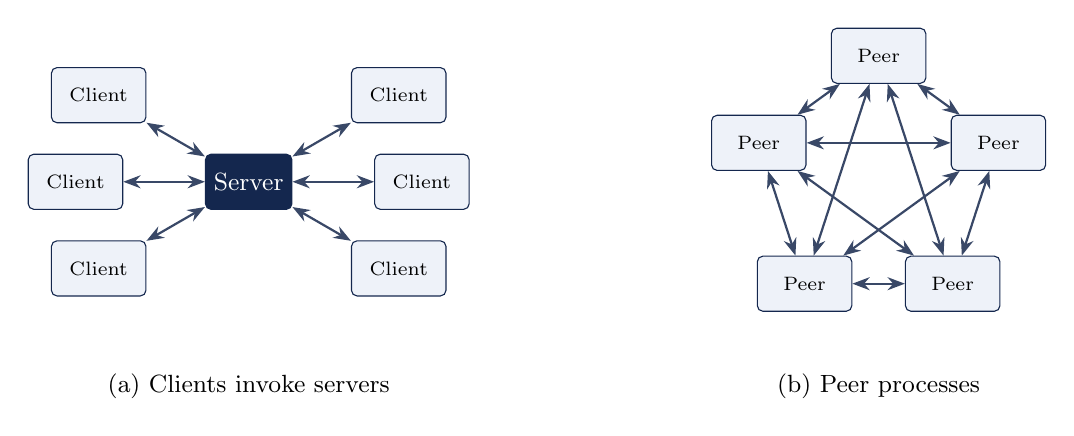
\begin{tikzpicture}
  % client-server
  \node[dark] (s) at (0,0) {Server};
  \foreach \i/\ang in {1/150,2/180,3/210,4/30,5/0,6/330}{
    \node[box,minimum width=1.2cm] (c\i) at ($(s)+(\ang:2.2cm)$) {\scriptsize Client};
    \draw[darr] (s)--(c\i);
  }
  \node at (0,-2.6) {\small (a) Clients invoke servers};
  % p2p
  \foreach \i/\ang in {1/90,2/162,3/234,4/306,5/18}{
    \node[box,minimum width=1.2cm] (p\i) at ($(8,0)+(\ang:1.6cm)$) {\scriptsize Peer};
  }
  \foreach \i/\j in {1/2,2/3,3/4,4/5,5/1,1/3,2/4,3/5,4/1,5/2}{
    \draw[darr] (p\i)--(p\j);
  }
  \node at (8,-2.6) {\small (b) Peer processes};
\end{tikzpicture}
\caption{Client-server versus peer-to-peer distributed applications.}
\end{figure}

\section{Grid Computing}
\begin{defbox}{Grid Computing}
\begin{itemize}[leftmargin=*]
  \item \textbf{Pcwebopedia:} harnesses \emph{unused processing cycles} of all computers in a
        network for problems too intensive for any stand-alone machine.
  \item \textbf{IBM:} enables the \emph{virtualization} of distributed computing and data
        resources (processing, network bandwidth, storage) to create a \emph{single system
        image}; a grid user sees one large virtual computer.
  \item \textbf{Sun Microsystems:} infrastructure providing \emph{dependable, consistent,
        pervasive and inexpensive} access to computational capabilities.
\end{itemize}
\end{defbox}

\textbf{Electrical power grid analogy.} Users plug into a wall socket without caring where the
electricity is generated; the power grid links many kinds of power plants. Likewise, grid users
get processors, storage, data and applications as needed with little or no knowledge of where
resources are or what hardware/OS lies beneath; ``the Grid'' links PCs, workstations, servers and
storage elements and provides the mechanism to access them.

\textbf{Features of grids:} (1) share more than information -- data, computing power and
applications in a dynamic, multi-institutional \emph{virtual organisation}; (2) efficient use of
resources at many institutes; (3) join local communities; (4) interaction with the underlying
layers must be \emph{transparent and seamless}.

\textbf{Need:} today's science is based on computation, data analysis, visualization and
collaboration; simulation and modelling are more cost effective than experiments; problems are
increasingly complex and need accurate solutions quickly; data visualization is important; and
under-utilised resources can be exploited.

\subsection{Types of Grids}
\begin{center}
\begin{tabularx}{\textwidth}{>{\bfseries}lX}
\toprule
Computational grid & Secure access to a huge pool of shared processing power for
high-throughput and computation-intensive applications.\\
Data grid & Infrastructure for storage, discovery, handling, publication and manipulation of
large data volumes stored in heterogeneous databases and file systems.\\
Collaboration grid & Supports collaboration, e.g.\ people from different companies in a virtual
enterprise working on components of a CAD project without disclosing proprietary technology.\\
Network grid & Fault-tolerant, high-performance communication; each node acts as a data router
providing caching to speed up communication.\\
Utility grid & Ultimate form: not only data and cycles but software and special equipment are
shared; applications run on one machine and users send data and receive results.\\
\bottomrule
\end{tabularx}
\end{center}

\section{Cluster Computing}
\begin{defbox}{Cluster}
A cluster is a type of parallel or distributed computer system consisting of a collection of
\textbf{inter-connected stand-alone computers} working together as a \textbf{single integrated
computing resource}. Key components: multiple standalone computers (PCs, workstations or SMPs),
operating systems, high-performance interconnects, middleware, parallel programming environments
and applications.
\end{defbox}
Clusters improve speed and/or reliability over a single computer and are more cost effective than
a single computer of comparable speed or reliability. In a typical cluster the network is faster
and closer than a LAN, uses low-latency protocols, and is \emph{more loosely coupled than SMP}.

\textbf{Types:} High Availability (failover) clusters; Load-Balancing clusters; Parallel/Distributed
processing clusters. \textbf{Components:} cluster nodes, cluster network, network characterisation.

\textbf{Benefits:} system availability (redundant hardware, OS and applications); hardware fault
tolerance (e.g.\ disk RAID); OS and application reliability; scalability (add servers or clusters);
high performance for cluster-enabled programs.

\begin{notebox}{Grid versus Cluster (Assignment 1, Q10)}
A \textbf{grid} is a form of distributed computing in which a large number of geographically
dispersed, often heterogeneous resources across multiple administrative domains are
\emph{loosely coupled} to work on a large-scale task. A \textbf{cluster} is tightly coupled and
co-located; a node is a single machine; a hypervisor is virtualization software.
\end{notebox}

\section{Utility Computing}
\begin{defbox}{Utility Computing}
Utility computing is a \emph{service provisioning model} in which a provider makes computing
resources and infrastructure management available to the customer as needed and charges for
\textbf{specific usage rather than a flat rate}. There is low or no initial cost; resources are
essentially rented. The analogy is electricity: fluctuating customer demand, charged by usage
(\emph{pay-per-use}). Utility computing is purely a concept which cloud computing practically
implements, usually with virtualization so that available storage/computing power is far larger
than that of a single time-sharing computer.
\end{defbox}

\textbf{Key elements:} (a) pay-for-use pricing model, (b) data-centre virtualization and
provisioning, (c) solves the resource-utilization problem, (d) outsourcing, (e) web services
delivery, (f) automation.

\textbf{Payment models:} flat rate, tiered, subscription, metered, pay-as-you-go, standing charges;
different customers get different models depending on scale, commitment and payment frequency; the
price expresses the provider's cost plus a profit margin.

\textbf{Risks:} data backup, data security, partner competency, defining the SLA, getting value
from charge-back.

\section{Cloud Computing: NIST Definition}
\begin{defbox}{Cloud Computing (NIST)}
Cloud computing is a model for enabling \textbf{ubiquitous, convenient, on-demand network access}
to a \textbf{shared pool of configurable computing resources} (e.g.\ networks, servers, storage,
applications and services) that can be \textbf{rapidly provisioned and released with minimal
management effort or service provider interaction}.
\end{defbox}

\subsection{Five Essential Characteristics}
\begin{enumerate}[leftmargin=*]
  \item \textbf{On-demand self-service:} a consumer can unilaterally provision capabilities such
        as server time and network storage automatically, without human interaction with each
        provider.
  \item \textbf{Broad network access:} capabilities are available over the network and accessed
        by standard mechanisms that promote use by heterogeneous thin or thick clients (mobile
        phones, tablets, laptops, workstations).
  \item \textbf{Resource pooling:} the provider's resources are pooled to serve many consumers
        using a \emph{multi-tenant model}, with physical and virtual resources dynamically
        assigned and reassigned according to demand.
  \item \textbf{Rapid elasticity:} capabilities can be elastically provisioned and released,
        sometimes automatically, to scale outward and inward with demand; to the consumer they
        often appear unlimited.
  \item \textbf{Measured service:} resource use is automatically controlled and optimised using a
        metering capability (storage, processing, bandwidth, active user accounts) and can be
        monitored, controlled and reported, giving transparency to provider and consumer.
\end{enumerate}

\subsection{Common Characteristics}
Massive scale, resilient computing, homogeneity, geographic distribution, virtualization,
service orientation, low-cost software, advanced security.

\begin{solved}{Identifying the characteristic}
\Given Statement: ``Computing resources are dynamically assigned to multiple customers using a
shared infrastructure.''
\Formula Match the statement to a NIST essential characteristic.
\Steps
\begin{enumerate}[leftmargin=*]
  \item Many customers share the same physical hardware $\Rightarrow$ multi-tenancy.
  \item Assignment and reassignment follows demand $\Rightarrow$ dynamic.
  \item These two properties together define \emph{resource pooling}.
\end{enumerate}
\Answer Resource pooling.
\end{solved}

\section{Cloud Service Models}
\begin{center}
\begin{tabularx}{\textwidth}{>{\bfseries}lXX}
\toprule
Model & Capability provided to the consumer & Consumer controls\\
\midrule
SaaS & Use provider's applications on cloud infrastructure via thin client (web browser) or
program interface. Example: Google Spreadsheet. & Nothing underneath; at most limited user-specific
configuration.\\
PaaS & Deploy consumer-created or acquired applications using languages, libraries, services and
tools supported by the provider. Examples: Microsoft Azure, Google App Engine. & Deployed
applications and possibly hosting-environment configuration; not network, servers, OS, storage.\\
IaaS & Provision processing, storage, networks and other fundamental resources; consumer deploys
arbitrary software. Examples: Amazon Web Services, Flexiscale, EC2. & OS, storage, deployed
applications and possibly some networking components.\\
\bottomrule
\end{tabularx}
\end{center}

\begin{figure}[H]
\centering
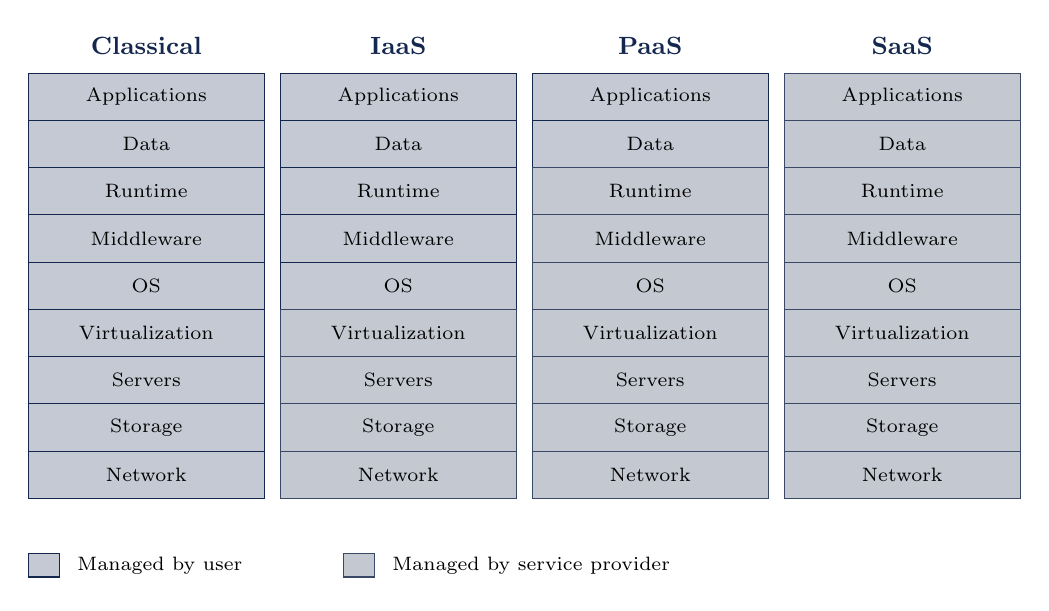
\begin{tikzpicture}[x=1cm,y=1cm]
  \foreach \kk/\xx/\nm in {9/0/Classical,5/3.2/IaaS,2/6.4/PaaS,0/9.6/SaaS}{
    \node[font=\bfseries\small,text=navy] at (\xx+1.5,0.35) {\nm};
    \foreach \rw/\lay in {1/Applications,2/Data,3/Runtime,4/Middleware,5/OS,6/Virtualization,7/Servers,8/Storage,9/Network}{
      \ifnum\rw>\kk
        \draw[fill=slate!30,draw=slate] (\xx,{-\rw*0.6}) rectangle ++(3,0.6);
      \else
        \draw[fill=navy!25,draw=navy] (\xx,{-\rw*0.6}) rectangle ++(3,0.6);
      \fi
      \node[font=\scriptsize] at (\xx+1.5,{-\rw*0.6+0.3}) {\lay};
    }
  }
  \fill[navy!25,draw=navy] (0,-6.4) rectangle ++(0.4,0.3);
  \node[anchor=west,font=\scriptsize] at (0.5,-6.25) {Managed by user};
  \fill[slate!30,draw=slate] (4,-6.4) rectangle ++(0.4,0.3);
  \node[anchor=west,font=\scriptsize] at (4.5,-6.25) {Managed by service provider};
\end{tikzpicture}
\caption{Responsibility split in the classical model, IaaS, PaaS and SaaS.}
\end{figure}

\begin{solved}{Classify the service model}
\Given A startup rents Amazon EC2 virtual servers; the team installs and patches its own OS,
configures the web server, manages runtime and applications. The provider supplies only
virtualized compute, storage and networking.
\Formula Service model = determined by the lowest layer the provider manages and the first layer the
consumer manages.
\Steps
\begin{enumerate}[leftmargin=*]
  \item Provider manages: virtualization, servers, storage, network.
  \item Consumer manages: OS, middleware/runtime, applications, data.
  \item This matches the right-most boundary of the IaaS column in the figure above.
\end{enumerate}
\Answer \textbf{IaaS}. SaaS (no consumer control), PaaS (OS is provider-managed) and FaaS are rejected.
\end{solved}

\subsection{Simplified Descriptions and Analogy}
SaaS applications are designed for end users and delivered over the web; PaaS is the set of tools
and services that makes coding and deploying applications quick and efficient; IaaS is the hardware
and software that powers it all -- servers, storage, networks, operating systems. In the
\textbf{transportation analogy}, roads are the infrastructure (IaaS), cars and trucks are the platform
(PaaS) and the people and goods are software and information (SaaS).

\section{Deployment Models}
\begin{itemize}[leftmargin=*]
  \item \textbf{Private cloud:} operated solely for one organization (e.g.\ Windows Server Hyper-V).
  \item \textbf{Community cloud:} shared by several organizations supporting a specific community goal.
  \item \textbf{Public cloud:} made available to the general public (e.g.\ Google Docs, Spreadsheet).
  \item \textbf{Hybrid cloud:} composition of two or more clouds (private, community or public),
        e.g.\ \emph{cloud bursting} for load balancing between clouds.
\end{itemize}

\section{Cloud and Virtualization}
\textbf{Virtual workspaces} are abstractions of an execution environment, dynamically available to
authorised clients through well-defined protocols, with a resource quota (CPU, memory share) and a
software configuration (OS). They are implemented on \textbf{virtual machines (VMs)}: an abstraction
of a physical host machine. A \textbf{hypervisor} (VMM) intercepts and emulates VM instructions and
manages VMs (VMware, Xen, KVM). Para-virtualization (e.g.\ Xen) approaches raw physical performance.

\begin{figure}[H]
\centering
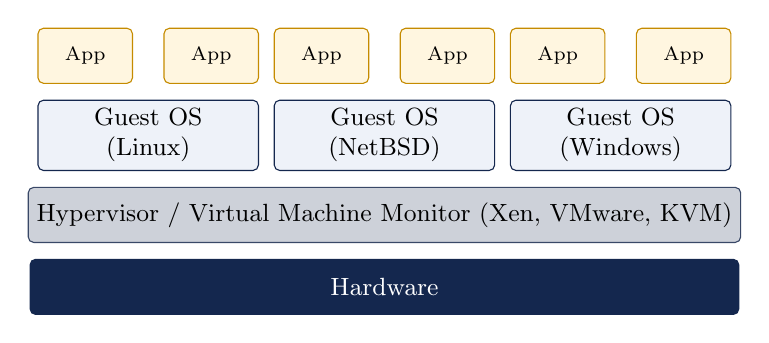
\begin{tikzpicture}
  \node[dark,minimum width=9cm] (hw) at (0,0) {Hardware};
  \node[mid,minimum width=9cm,above=2mm of hw] (hv) {Hypervisor / Virtual Machine Monitor (Xen, VMware, KVM)};
  \node[box,minimum width=2.8cm,above=2mm of hv,xshift=-3cm] (g1) {Guest OS\\(Linux)};
  \node[box,minimum width=2.8cm,above=2mm of hv] (g2) {Guest OS\\(NetBSD)};
  \node[box,minimum width=2.8cm,above=2mm of hv,xshift=3cm] (g3) {Guest OS\\(Windows)};
  \foreach \g in {g1,g2,g3}{
    \node[gold,minimum width=1.2cm,above=2mm of \g.north west,anchor=south west] {\scriptsize App};
    \node[gold,minimum width=1.2cm,above=2mm of \g.north east,anchor=south east] {\scriptsize App};
  }
\end{tikzpicture}
\caption{Virtualized stack: several guest operating systems share one physical machine.}
\end{figure}

\textbf{Advantages of VMs:} run OSs where physical hardware is unavailable; easy to create and back up
machines; software testing on clean installs; emulate more machines than physically available;
timeshare lightly loaded systems on one host; debug by suspend/resume; easy migration; run legacy
systems.

\begin{solved}{Virtualization statements}
\Given Four statements about VMs and hypervisors.
\Formula A VM provides a virtual machine with its own guest OS; Type-1 hypervisors run on bare metal,
Type-2 run as applications on a host OS.
\Steps
\begin{enumerate}[leftmargin=*]
  \item ``Each VM always shares the host kernel'' describes \emph{containers}, not VMs -- false.
  \item Multiple VMs can run different OSs simultaneously on one machine -- \textbf{true}.
  \item Virtualization pre-dates cloud, so ``only possible in cloud'' is false.
  \item Overcommitment (CPU/memory) is a commonly used feature, not something virtualization prevents.
  \item Type-2 (hosted) hypervisors (VirtualBox, VMware Workstation) run as an application on a host OS.
\end{enumerate}
\Answer VMs of different OSs coexist (Q4: B); Type-2 hypervisor runs on top of a host OS (Q7: B).
\end{solved}

\section{Cloud-sourcing, Cloud Storage, Advantages and Disadvantages}
\textbf{Why cloud-sourcing matters:} high-scale low-cost providers, any time/place access via browser,
rapid scalability with incremental cost and load sharing, and no need to focus on local IT.
\textbf{Concerns:} performance, reliability and SLAs; control of data and service parameters;
application features and choices; interaction between providers; no standard API (mix of SOAP and REST);
privacy, security, compliance, trust.
\textbf{Cloud storage:} large web companies rent out spare storage (e.g.\ Amazon EC2 and S3).

\subsection{Advantages}
Lower computer costs; improved performance; reduced software costs; instant software updates; improved
document-format compatibility; unlimited storage capacity (hundreds of petabytes versus a 1~TB drive);
increased data reliability (e.g.\ Dropbox, SkyDrive); universal information access; latest-version
availability; easier group collaboration; device independence.

\subsection{Disadvantages}
Requires a constant Internet connection; does not work well with low-speed connections; features may be
limited (e.g.\ PowerPoint versus web presentation tools); can be slow; stored data might not be secure;
stored data can be lost; HPC applications using MPI/OpenMP are difficult (co-location of VMs needed to
minimise latency); general concerns -- different protocols and APIs per cloud, proprietary database and
workflow systems requiring application adaptation.

\section{Business Drivers and Cloud Economics (Introductory)}
Public clouds can significantly reduce IT cost. To the end user, the cloud gives the illusion of
potentially infinite capacity with rapid scale and pay-per-use. In contrast, private data centres must be
\emph{provisioned for peak capacity}, giving a low average utilization of \textbf{5--20\%}.

\begin{center}
\begin{tabular}{lrr}
\toprule
 & In-house server & Cloud server\\
\midrule
Purchase cost & \$9600 & 0\\
Cost/hr (over 3 years) & \$0.36 & \$0.68\\
Cost ratio Cloud/In-house & \multicolumn{2}{c}{1.88}\\
Efficiency & 40\% & 80\%\\
Cost per effective hour & \$0.90 & \$0.85\\
Power and cooling & \$0.36 & 0\\
Management cost & \$0.10 & \$0.01\\
\textbf{Total cost/effective hour} & \textbf{\$1.36} & \textbf{\$0.86}\\
Cost ratio In-house/Cloud & \multicolumn{2}{c}{1.58}\\
\bottomrule
\end{tabular}
\end{center}
The in-house server in the table is an x86 machine with three quad-core processors, 12~GB RAM and a 300~GB disk.

\begin{solved}{IaaS economics: why the dearer cloud server is cheaper per useful hour}
\Given In-house: \$0.36/hr, efficiency 40\%, power and cooling \$0.36, management \$0.10.
Cloud: \$0.68/hr, efficiency 80\%, power and cooling \$0, management \$0.01.
\Formula Cost per effective hour $= \dfrac{\text{cost per hour}}{\text{efficiency}}$;\quad
total $=$ cost per effective hour $+$ power and cooling $+$ management.
\Steps
\begin{enumerate}[leftmargin=*]
  \item In-house: $0.36/0.40 = 0.90$; total $= 0.90 + 0.36 + 0.10 = 1.36$.
  \item Cloud: $0.68/0.80 = 0.85$; total $= 0.85 + 0 + 0.01 = 0.86$.
  \item Raw price ratio: $0.68/0.36 = 1.88$ (cloud dearer per hour).
  \item Total ratio: $1.36/0.86 = 1.58$.
\end{enumerate}
\Answer Total cost per effective hour: in-house \$1.36, cloud \$0.86, ratio $\approx 1.58$ in favour of the cloud.
\end{solved}

\textbf{Benefits for end users of public cloud:} high utilization and scalability; no hardware
procurement; no power cost; no IT administration; user-friendly SLAs (about 99\% availability with
compensation on a miss); rent to prototype before investing; portability standards (Cloud Computing
Interoperability Forum, Open Cloud Consortium; Amazon EC2 and Eucalyptus share the same API);
startups avoid capital investment. \textbf{Benefits for SMBs (fewer than 250 employees)} follow the same
lines. \textbf{Benefits of private cloud:} one 12-core 12~GB server costs far less than twelve 1-core 1~GB
servers; data confidentiality preserved; VMs cheaper and faster to provision than physical machines.

\textbf{Economics of PaaS versus IaaS:} for a 24x7 web application with unpredictable volume, IaaS requires
a minimum set of servers always provisioned, while deploying on PaaS costs nothing at rest, costs are
incurred by usage, and the platform scales automatically. \textbf{PaaS benefits:} no scaling or load
balancing by the user; web-based IDE; easier migration from development to production; no separate IDE
licences. \textbf{SaaS benefits:} subscribe instead of buying and licensing software; use free tools such as
Google Docs; enterprises use web-based CRM instead of installing servers.

\textbf{Purposes of cloud in organizations:} IT platform for multi-organization processes; backup; CRM,
ERP, supply-chain; personal productivity and collaboration; development and test; storing and archiving
large files; analysing customer/operations data; e-business and e-government sites; R\&D analysis; handling
demand spikes; batch processing (conversion, risk modelling, rendering); sharing information with
regulators; consumer entertainment. \textbf{Top cloud applications:} mail and messaging, archiving, backup,
storage, security, virtual servers, CRM, cross-enterprise collaboration, hosted PBX, video conferencing.

\section{Cloud Computing Architecture}
\subsection{Building Blocks}
\begin{itemize}[leftmargin=*]
  \item \textbf{Technical architecture:} structuring by the XaaS stack; adopting cloud paradigms;
        structuring services and components; relationships and external endpoints; middleware and
        communication; management and security.
  \item \textbf{Deployment/operation architecture:} geo-location check (legal issues, export control);
        operation and monitoring.
\end{itemize}

\subsection{XaaS}
\begin{defbox}{XaaS}
Combining Service-Oriented Infrastructure (SOI) with cloud computing realises \textbf{XaaS}: ``anything'' or
``everything'' as a Service -- a growing number of services delivered over the Internet rather than
locally. \textbf{Broad network access + resource pooling (cloud) + business-driven infrastructure on demand +
service orientation (SOI) = XaaS}, which fulfils the CSP demands: increase productivity, end-user
satisfaction, innovation and agility.
\end{defbox}
Other XaaS examples: Business Process as a Service (BPaaS), Storage as a Service, Security as a Service
(SECaaS), Database as a Service (DaaS), Monitoring/Management as a Service (MaaS), Communications, Content and
Computing as a Service (CaaS), Identity as a Service (IDaaS), Backup as a Service (BaaS), Desktop as a Service.

\begin{notebox}{Assignment 1, Q6}
The combination of SOA and cloud computing leading to ``almost any IT capability delivered as a service'' is
called \textbf{XaaS}. FaaS (Functions as a Service) is just one specific model.
\end{notebox}

\subsection{Classical (Legacy) Model versus Evergreen IT}
In the classical model all layers (hardware, OS, development tools, applications) are managed by users who
bear the hardware, maintenance and technology cost; systems are custom build-to-order, deployed as
tightly coupled vertical stacks of layers (no single part easily replaced), with manual provisioning --
\emph{Legacy IT}. Cloud simplifies the stack towards \emph{Evergreen IT}: dedicated infrastructure,
application and end-user devices form a simplified IT stack.

\subsection{Client-Server Model versus Cloud Model}
\begin{center}
\begin{tabularx}{\textwidth}{>{\bfseries}XXX}
\toprule
 & Client-server model & Cloud computing model\\
\midrule
Service model & Simple: server services client requests & Variety of complex models (IaaS, PaaS, SaaS)\\
Load balancing & May or may not be load balanced & Load balanced\\
Scalability & Scalable to some extent in a cluster & Theoretically infinitely scalable\\
Virtualization & No concept of virtualization & Virtualization is the core concept\\
\bottomrule
\end{tabularx}
\end{center}
A three-tier client-server architecture has presentation, application and data tiers; the client is often a
thin client, and the server may be a load-balanced cluster or a stand-alone machine.

\subsection{SaaS, PaaS, IaaS in Detail}
\begin{center}
\begin{tabularx}{\textwidth}{>{\bfseries}lXXX}
\toprule
 & SaaS & PaaS & IaaS\\
\midrule
Definition & Software deployed over the Internet, licensed on demand, by subscription, pay-as-you-go, or free
(ad/user-list revenue). & Platform for creating web applications quickly without buying and maintaining
underlying software and infrastructure. & Servers, storage, network and OS delivered as an on-demand,
outsourced service.\\
Characteristics & Web access to commercial software; managed from a central location; one-to-many delivery;
no upgrades or patches by users; APIs for integration. & Integrated development, test, deploy, host and
maintain services; web-based UI tools; multi-tenant; built-in scalability, load balancing and failover;
web-service/database integration; team collaboration; billing and subscription tools. & Resources
distributed as a service; dynamic scaling; variable utility pricing; multiple users per hardware.\\
Good fit & Interplay with the outside world (e.g.\ email campaigns); web/mobile access; short-term use;
demand spikes (tax/billing); e.g.\ Salesforce CRM. & Multiple developers or external parties; automated
test and deployment; agile development; e.g.\ Azure, Google App Engine. & Volatile demand; new
organizations without capital; rapid growth; limiting CAPEX in favour of OPEX; trial or temporary needs.\\
Poor fit & Extremely fast real-time processing; regulations forbidding external hosting; existing on-premise
solution suffices. & Highly portable applications; proprietary languages causing lock-in; need to
customise underlying hardware/software. & Regulatory limits on offshoring/outsourcing data; highest
performance needs met by on-premise hardware.\\
\bottomrule
\end{tabularx}
\end{center}

\begin{solved}{Advantages of PaaS}
\Given Four claimed advantages: (i) developers focus on application development, (ii) automatic software
updates of the underlying platform, (iii) complete control over physical server hardware, (iv) faster
application deployment.
\Formula PaaS abstracts infrastructure management and offers managed runtime environments.
\Steps
\begin{enumerate}[leftmargin=*]
  \item (i) true -- infrastructure is abstracted. (ii) true -- the provider updates the platform.
  \item (iii) false -- physical hardware is the provider's responsibility.
  \item (iv) true -- ready-made runtime and IDE speed deployment.
\end{enumerate}
\Answer (i), (ii) and (iv)
\end{solved}

\section{Role of Networking and Network Function Virtualization}
Network resources can be provisioned dynamically in the cloud. Core concepts: Virtual LANs, Virtual
Private Networks and protocol layers; tools such as OpenSSH and OpenVPN set up topologies and
configurations.

\begin{defbox}{Network Functions Virtualisation (ETSI NFV)}
NFV aims to transform how operators architect networks by evolving standard IT virtualisation technology to
consolidate many network-equipment types onto industry-standard high-volume servers, switches and storage in
data centres, network nodes and end-user premises. Network functions are implemented in software that can be
moved to, or instantiated in, various locations as required, without installing new equipment.
\end{defbox}

\section{Week 1 Assignment Review}
\begin{center}
\begin{tabularx}{\textwidth}{cXc}
\toprule
Q & Concept tested & Answer\\
\midrule
1 & Resource pooling (multi-tenant shared resources) & B\\
2 & EC2 rented VM with user-managed OS $\Rightarrow$ IaaS & C\\
3 & Private cloud: exclusive use, on-premises or third-party hosted & D\\
4 & Different OS VMs simultaneously on one machine & B\\
5 & Distributed systems: scalability and fault tolerance, \emph{not} guaranteed lower latency & A\\
6 & SOA + cloud $\Rightarrow$ XaaS & C\\
7 & Type-2 hypervisor runs as an application on a host OS & B\\
8 & PaaS advantages (i), (ii), (iv) & A\\
9 & Amazon EC2 is IaaS & B\\
10 & Grid: geographically dispersed, heterogeneous, loosely coupled & B\\
\bottomrule
\end{tabularx}
\end{center}

\begin{solved}{Distributed system statements}
\Given (i) adding nodes improves scalability; (ii) replication increases fault tolerance;
(iii) distribution guarantees lower latency for every operation than a centralized system.
\Formula Distribution adds network communication and coordination overhead.
\Steps
\begin{enumerate}[leftmargin=*]
  \item (i) True: horizontal scaling.
  \item (ii) True: replication of data and services.
  \item (iii) False: remote calls and coordination can make some operations slower.
\end{enumerate}
\Answer (i) and (ii) only
\end{solved}

% ==================================================================
%  WEEK 2
% ==================================================================
\chapter{Deployment Models, Virtualization, XML and Web Services}

\section{Deployment Models in Depth}
\begin{center}
\begin{tabularx}{\textwidth}{>{\bfseries}lXX}
\toprule
Model & Definition & Examples\\
\midrule
Public & Infrastructure provisioned for open use by the general public; owned, managed and operated by a
business, academic or government organization; exists on the provider's premises. & Google App Engine,
Microsoft Windows Azure, IBM SmartCloud, Amazon EC2\\
Private & Provisioned for exclusive use by a single organization with multiple consumers (business
units); owned and operated by the organization, a third party or both; on or off premises. & Eucalyptus,
Ubuntu Enterprise Cloud, Amazon VPC, VMware Cloud Infrastructure Suite\\
Community & Provisioned for a specific community with shared concerns (mission, security, policy,
compliance); owned and operated by one or more members, a third party, or both. & Google Apps for
Government, Microsoft Government Community Cloud\\
Hybrid & Composition of two or more distinct clouds (private, community, public) that remain unique
entities but are bound by standardized or proprietary technology enabling data and application
portability. & Windows Azure (hybrid capable), VMware vCloud\\
\bottomrule
\end{tabularx}
\end{center}

\subsection{Public Cloud: Issues}
\begin{itemize}[leftmargin=*]
  \item \textbf{Hidden workload location:} the provider may migrate workloads anywhere at any time
        (e.g.\ to low-cost data centres) unless location-restriction policies are offered.
  \item \textbf{Multi-tenancy risk:} a machine may host workloads of competitors or adversaries
        (reliability and security risk).
  \item \textbf{Network dependency:} access over the public Internet depends on DNS servers, router
        infrastructure and inter-router links.
  \item \textbf{Limited visibility and control:} provider operations and software are proprietary; a
        subscriber cannot verify complete deletion of data.
  \item \textbf{Elasticity:} illusion of unlimited resources; high flexibility in moving workloads.
  \item \textbf{Low up-front cost}, but \textbf{restrictive default SLAs}.
\end{itemize}

\subsection{Private Cloud: On-site versus Outsourced}
\begin{center}
\begin{tabularx}{\textwidth}{>{\bfseries}lXX}
\toprule
Aspect & On-site private & Outsourced private\\
\midrule
Security perimeter & One perimeter around subscriber resources and private cloud & Two perimeters
(subscriber and provider) joined by a protected link; security depends on both and the link\\
Up-front cost & Significant to high (install and manage cloud software even if free) & Modest to
significant (negotiating SLA, upgrading network, porting, training)\\
Resources & Fixed capacity sized for anticipated workloads & Extensive; rent any quantity offered\\
Data import/export & Limited by on-site network capacity & Limited by provider-subscriber link, but
adjustable by provisioning high-performance links\\
IT skills & Traditional plus cloud IT skills required & Less in-house operation\\
Multi-tenancy & Workloads of different clients separated only by access policies; a software or policy
flaw can expose workloads & Same implications\\
\bottomrule
\end{tabularx}
\end{center}

\subsection{Community and Hybrid Clouds}
In a community cloud, each participant organization may provide services, consume services, or both
(at least one must provide) and each implements its own security perimeter; perimeters are linked by
boundary controllers. Access policy can be complex: with $N$ members a sharing decision must be made
between each pair, expressed with role-based (RBAC) or attribute-based access control. Costs for a
participant vary widely depending on whether it consumes only or also provides. An \emph{outsourced
community cloud} resembles an outsourced private cloud but with multiple protected links.
A hybrid cloud can be extremely complex and may change over time as constituent clouds join and leave.

\section{IaaS: Provider-Subscriber View and Architecture}
A subscriber gets access to virtual computers, network-accessible storage, network components such as
firewalls, and configuration services. Fees are typically per CPU-hour, GB stored per hour, bandwidth,
network infrastructure used (e.g.\ IP addresses per hour) and value-added services (monitoring,
auto-scaling). The provider keeps spare VMs (e.g.\ clients A, B, C hold vm1--vm6 while the provider
retains vm7--vmN).

\textbf{Scope of control:} the IaaS stack comprises hardware, OS (split into a privileged hypervisor/VMM layer and
a guest OS layer), middleware and applications. The provider keeps total control of hardware and
administrative control of the hypervisor; the subscriber controls the guest OS, middleware and
applications and may load any supported OS image. A hypervisor synthesizes VMs, each \emph{``an efficient,
isolated duplicate of a real machine''}.

\subsection{Three-level Hierarchy}
\begin{figure}[H]
\centering
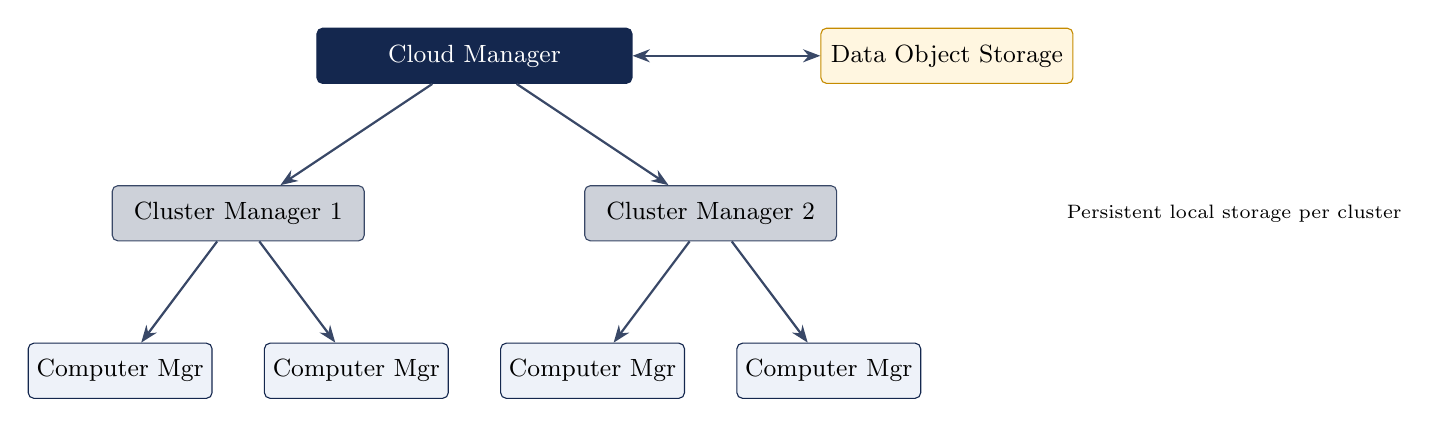
\begin{tikzpicture}
  \node[dark,minimum width=4cm] (cm) at (0,0) {Cloud Manager};
  \node[gold,minimum width=3.2cm] (dos) at (6,0) {Data Object Storage};
  \node[mid,minimum width=3.2cm] (c1) at (-3,-2) {Cluster Manager 1};
  \node[mid,minimum width=3.2cm] (c2) at (3,-2) {Cluster Manager 2};
  \node[box,minimum width=2.2cm] (n1) at (-4.5,-4) {Computer Mgr};
  \node[box,minimum width=2.2cm] (n2) at (-1.5,-4) {Computer Mgr};
  \node[box,minimum width=2.2cm] (n3) at (1.5,-4) {Computer Mgr};
  \node[box,minimum width=2.2cm] (n4) at (4.5,-4) {Computer Mgr};
  \draw[arr] (cm)--(c1); \draw[arr] (cm)--(c2);
  \draw[arr] (c1)--(n1); \draw[arr] (c1)--(n2); \draw[arr] (c2)--(n3); \draw[arr] (c2)--(n4);
  \draw[darr] (cm)--(dos);
  \node[font=\scriptsize,anchor=west] at (7.4,-2) {Persistent local storage per cluster};
\end{tikzpicture}
\caption{Logical view of an IaaS cloud: top, middle and bottom levels.}
\end{figure}

\begin{itemize}[leftmargin=*]
  \item \textbf{Cloud Manager:} public access point where subscribers sign up, manage rented resources and
        access data; authenticates subscribers, generates/validates access credentials, performs top-level
        resource management, and decides if the cloud has enough free resources.
  \item \textbf{Data Object Storage (DOS):} stores subscriber metadata such as credentials and OS images;
        usually one service per cloud.
  \item \textbf{Cluster Manager:} manages a collection of computers on a high-speed LAN (clusters may be
        geographically distributed); receives allocation commands from the Cloud Manager, queries Computer
        Managers for availability, instructs allocation, and reconfigures virtual networking; attached to
        \emph{Persistent Local Storage (PLS)} giving disk-like storage to VMs.
  \item \textbf{Computer Manager:} runs on each host; uses virtualization to provide VMs; tracks how many VMs
        run and how many can start; uses the hypervisor command interface to start, stop, suspend and
        reconfigure VMs.
\end{itemize}

\begin{solved}{Capacity check by the hierarchy}
\Given Two clusters, each with 10 computers; each computer can host at most 8 VMs; 60 VMs already running; a subscriber requests 25 more VMs.
\Formula Free slots $=$ (clusters $\times$ computers $\times$ slots) $-$ running VMs.
\Steps
\begin{enumerate}[leftmargin=*]
  \item Total capacity $= 2 \times 10 \times 8 = 160$ VM slots.
  \item Free slots $= 160 - 60 = 100$.
  \item The Cluster Managers report availability upward; $25 \le 100$, so the Cloud Manager can satisfy the request.
\end{enumerate}
\Answer Request accepted; 75 slots remain free after allocation.
\end{solved}

\section{Virtualization}
Virtualization lets one computer do the job of several by sharing a single hardware platform among multiple
isolated environments; the focus here is \emph{platform virtualization}. Unlike dual-boot, both OSes run
\emph{simultaneously} and are completely isolated.

\subsection{Hypervisor and Popek--Goldberg Requirements}
A hypervisor runs the guest OS directly on the CPU in user mode, so privileged instructions must be
intercepted. Popek and Goldberg (CACM 1974) give three goals:
\begin{itemize}[leftmargin=*]
  \item \textbf{Equivalence:} VM indistinguishable from the real hardware.
  \item \textbf{Resource control:} VMM fully controls virtualized resources.
  \item \textbf{Efficiency:} most instructions execute directly on the CPU without the hypervisor.
\end{itemize}
Instructions are \emph{privileged} (trap in user mode) or \emph{sensitive} (change underlying resources --
\emph{control sensitive}, or reveal the privilege level -- \emph{behavior sensitive}).

\begin{thmbox}{Popek--Goldberg theorem}
For any conventional third-generation computer, a VMM may be constructed if the set of sensitive
instructions is a \textbf{subset} of the set of privileged instructions:
\[ \text{Sensitive} \subseteq \text{Privileged}. \]
A machine is \emph{recursively virtualizable} if it is virtualizable and a VMM without timing dependencies
can be built for it.
\end{thmbox}

\begin{figure}[H]
\centering
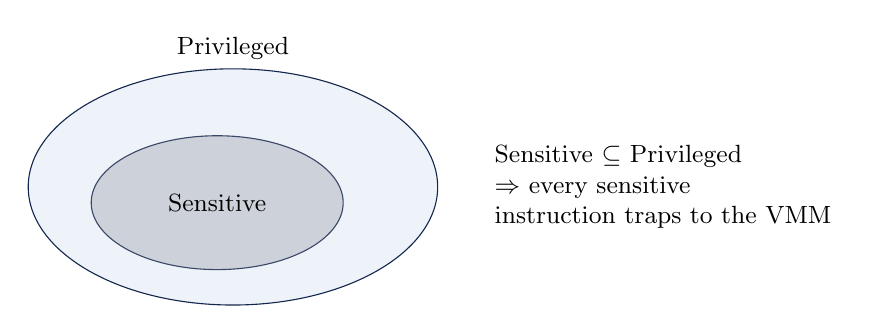
\begin{tikzpicture}
  \draw[fill=paleblue,draw=navy] (0,0) ellipse (2.6cm and 1.5cm);
  \node[font=\small,anchor=south] at (0,1.5) {Privileged};
  \draw[fill=slate!25,draw=slate] (-0.2,-0.2) ellipse (1.6cm and 0.85cm);
  \node[font=\small] at (-0.2,-0.2) {Sensitive};
  \node[font=\small,align=left,anchor=west] at (3.2,0) {Sensitive $\subseteq$ Privileged\\$\Rightarrow$ every sensitive\\instruction traps to the VMM};
\end{tikzpicture}
\caption{Virtualizable architecture: sensitive instructions lie inside the privileged set.}
\end{figure}

\begin{solved}{Is the instruction set virtualizable?}
\Given Architecture A: privileged $=\{\texttt{HLT},\texttt{LGDT},\texttt{OUT},\texttt{IN},\texttt{LIDT}\}$, sensitive $=\{\texttt{LGDT},\texttt{OUT},\texttt{IN}\}$.
Architecture B: same privileged set, sensitive $=\{\texttt{LGDT},\texttt{OUT},\texttt{POPF}\}$ where \texttt{POPF} silently ignores flag changes in user mode.
\Formula VMM constructible iff Sensitive $\subseteq$ Privileged.
\Steps
\begin{enumerate}[leftmargin=*]
  \item A: all three sensitive instructions appear in the privileged set, so subset holds.
  \item B: \texttt{POPF} is sensitive but not privileged (does not trap), so the subset fails.
\end{enumerate}
\Answer A is classically virtualizable; B is not (needs binary translation or hardware assistance).
\end{solved}

\subsection{Approaches to Server Virtualization}
\begin{center}
\begin{tabularx}{\textwidth}{>{\bfseries}lXXX}
\toprule
 & Full virtualization & Para-virtualization & Hardware-assisted\\
\midrule
Generation & 1st (binary rewriting, software based) & 2nd (cooperative) & 3rd (silicon based)\\
Guest OS & Unmodified; unaware of emulation & \textbf{Modified}; uses hypercalls/specialized API &
Unmodified\\
Mechanism & Dynamic binary translation; all hardware including CPU emulated (QEMU, Bochs) & Guest runs
kernel operations at ring 1; no privileged-instruction translation by VMM & CPU extensions (Intel VT-x,
AMD-V) intercept privileged operations; guest at ring 0, VMM in a more privileged ``ring $-1$''\\
Pros & Isolation; total VM portability across dissimilar hosts & Low overhead, close to native & Runs
legacy unmodified OSs\\
Cons & Emulation performance cost; guest forced to ring 1/3 so VMM must trap and emulate & Requires modified OS or
para-virtual drivers (recompiling kernel or installing drivers) & Speed/flexibility: unmodified OS cannot
exploit virtualization features (partly solved by para-virtual drivers)\\
\bottomrule
\end{tabularx}
\end{center}

\begin{figure}[H]
\centering
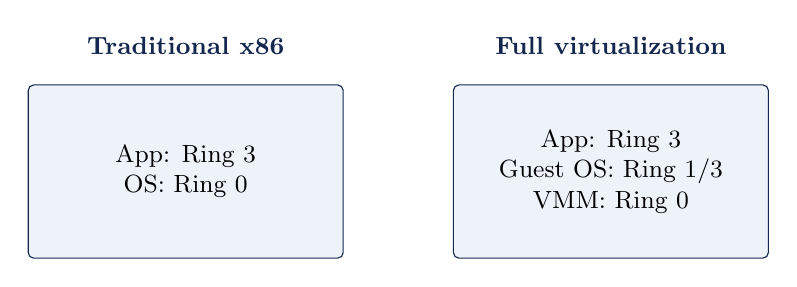
\begin{tikzpicture}[x=1cm,y=1cm]
  \foreach \xx/\ttl/\rings in {0/{Traditional x86}/{App: Ring 3\\OS: Ring 0},
                               5.4/{Full virtualization}/{App: Ring 3\\Guest OS: Ring 1/3\\VMM: Ring 0}}{
    \node[font=\bfseries\small,text=navy] at (\xx+2,1.6) {\ttl};
    \node[box,minimum width=4cm,minimum height=2.2cm,align=center] at (\xx+2,0) {\rings};
  }
\end{tikzpicture}
\caption{Privilege rings: full virtualization forces the guest kernel out of ring 0.}
\end{figure}

\begin{solved}{Para-virtualization recognition (Assignment 2, Q1, Q2)}
\Given A guest OS must issue \emph{hypercalls} instead of executing certain privileged instructions.
\Formula Hypercalls $\Leftrightarrow$ modified guest OS $\Leftrightarrow$ para-virtualization.
\Steps
\begin{enumerate}[leftmargin=*]
  \item Full / hardware-assisted virtualization runs an \emph{unmodified} guest; privileged instructions handled
        by hypervisor and VT-x/AMD-V.
  \item Hypercalls require OS modification, reducing overhead.
\end{enumerate}
\Answer Para-virtualization (Q1: C). Full virtualization is characterised by an unmodified guest with
CPU extensions and hypervisor (Q2: B).
\end{solved}

\subsection{Host OS, Guest OS and Hypervisor}
The hypervisor creates and manages VMs; each guest OS runs inside a VM; for a Type-2 hypervisor the host OS is
the OS on which the hypervisor runs (Assignment 2, Q5: B).

\section{Network Virtualization}
Network virtualization makes one physical network appear as multiple logical networks.
\textbf{Motivation:} the Internet is ``paralyzed'' by makeshift fixes (overlays); a one-size-fits-all
architecture is hard, so build an \emph{all-sizes-fit-into-one} open, expandable architecture and a testbed for
future protocols. \textbf{Related concepts:} VPNs (not customizable enough), active and programmable networks,
overlay networks (not flexible enough).

\begin{itemize}[leftmargin=*]
  \item \textbf{Business model roles:} Infrastructure Providers (InPs) manage physical networks; Service
        Providers (SPs) create virtual networks and deploy end-to-end services; End Users buy services; Brokers
        mediate.
  \item \textbf{Design principles:} concurrence of multiple heterogeneous virtual networks; recursion; inheritance
        of architectural attributes; revisitation of virtual nodes.
  \item \textbf{Design goals:} flexibility; manageability (policy separated from mechanism); scalability;
        security, privacy and isolation; programmability; heterogeneity; experimental and deployment
        facility (PlanetLab, GENI, VINI); legacy support.
\end{itemize}

\begin{defbox}{Network Virtualization}
A networking environment that allows multiple service providers to dynamically compose multiple heterogeneous
virtual networks that coexist in isolation, to deploy customized end-to-end services on the fly and manage them
for end users, by effectively sharing underlying network resources leased from multiple infrastructure providers.
\end{defbox}

\begin{figure}[H]
\centering
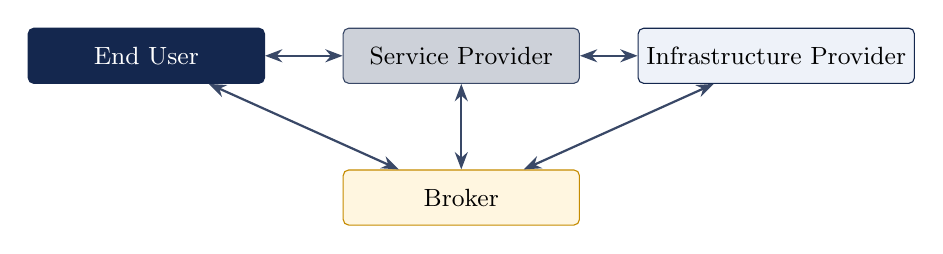
\begin{tikzpicture}
  \node[dark,minimum width=3cm] (u) at (0,0) {End User};
  \node[mid,minimum width=3cm] (sp) at (4,0) {Service Provider};
  \node[box,minimum width=3cm] (inp) at (8,0) {Infrastructure Provider};
  \node[gold,minimum width=3cm] (br) at (4,-1.8) {Broker};
  \draw[darr] (u)--(sp); \draw[darr] (sp)--(inp);
  \draw[darr] (br)--(sp); \draw[darr] (br)--(u); \draw[darr] (br)--(inp);
\end{tikzpicture}
\caption{Business model of network virtualization.}
\end{figure}

\section{XML: eXtensible Markup Language}
XML is a syntax for encoding text-based data using printable Unicode characters. It is \textbf{extensible} (you define
your own elements within the syntax rules) and a \textbf{universal format}: syntax rules ensure all processing
software handles a given document identically. The data model is a \textbf{tree} of elements, attributes and text; it is
self-describing, designed for distributed environments and can mix vocabularies.

\begin{lstlisting}[language=XML]
<?xml version="1.0" encoding="utf-8"?>
<partorders>
  <order ref="x23-2112-2342" date="25aug1999-12:34:23h">
    <desc>Gold sprockel grommets</desc>
    <part number="23-23221-a12" />
    <quantity units="gross">12</quantity>
    <deliveryDate date="27aug1999-12:00h" />
  </order>
</partorders>
\end{lstlisting}

\begin{figure}[H]
\centering
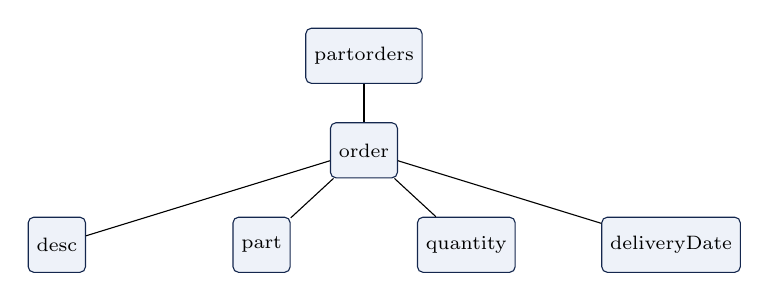
\begin{tikzpicture}[level distance=1.2cm,sibling distance=2.6cm,every node/.style={box,font=\scriptsize}]
  \node {partorders} child {node {order}
      child {node {desc}} child {node {part}} child {node {quantity}} child {node {deliveryDate}}};
\end{tikzpicture}
\caption{XML data model: a hierarchical tree.}
\end{figure}

\subsection{Well-formedness, Entities and Parsers}
\begin{itemize}[leftmargin=*]
  \item \textbf{Well-formed:} syntactically correct; the minimal requirement ``to be'' XML. A parser \emph{must stop}
        (raise an exception) if data is not well-formed.
  \item \textbf{Internal entities} (declared in the DTD, e.g.\ \verb|<!ENTITY messageHeader "...">|, referenced as
        \verb|&messageHeader;|) and \textbf{external entities} (\verb|SYSTEM "URL"|, shared among documents).
        References are replaced recursively.
  \item \textbf{Validating parser:} must retrieve all entities and process all DTD content, stopping on failure.
        \textbf{Non-validating parser:} tries to retrieve entities but stops DTD processing at the first missing
        one without error.
  \item \textbf{Characters:} use character references such as \verb|&#9824;| for characters outside the encoding;
        binary data must be encoded as printable characters.
\end{itemize}

\begin{solved}{Well-formed or not?}
\Given Documents: (1) \verb|<a><b>x</b></a>|; (2) \verb|<a><b>x</a></b>|; (3) \verb|<a x=1/>|; (4) \verb|<a x="1"/>|.
\Formula Well-formed: single root, properly nested tags, all tags closed, attribute values quoted.
\Steps
\begin{enumerate}[leftmargin=*]
  \item (1) properly nested -- well-formed.
  \item (2) tags overlap -- not well-formed.
  \item (3) unquoted attribute value -- not well-formed.
  \item (4) quoted attribute, empty element closed -- well-formed.
\end{enumerate}
\Answer (1) and (4) are well-formed; (2) and (3) force a parser to halt.
\end{solved}

\subsection{DTD, XML Schema and Namespaces}
\textbf{Well-formed} means syntactically correct; \textbf{valid} means well-formed and consistent with a DTD or Schema.
A DTD specifies allowed element and attribute names, nesting rules and content restrictions.

\begin{lstlisting}[language=XML]
<!DOCTYPE transfers [
  <!ELEMENT transfers (fundsTransfer)+>
  <!ELEMENT fundsTransfer (from, to)>
  <!ATTLIST fundsTransfer date CDATA #REQUIRED>
  <!ELEMENT from (amount, transitID?, accountID, acknowledgeReceipt)>
  <!ATTLIST from type (intrabank|internal|other) #REQUIRED>
  <!ELEMENT amount (#PCDATA)>
  <!ELEMENT to EMPTY>
  <!ATTLIST to account CDATA #REQUIRED>
]>
\end{lstlisting}

\begin{center}
\begin{tabularx}{\textwidth}{>{\bfseries}lXX}
\toprule
 & DTD & XML Schema (2001)\\
\midrule
Syntax & Special DTD grammar (part of core XML) & Pure XML\\
Types & Limited (CDATA, PCDATA) & Integers, dates, real numbers in a range, enumerations\\
Entities & Can declare entities & Cannot declare entities\\
Use & Basic structure validation & Type validation; relating database schemas to XML models\\
\bottomrule
\end{tabularx}
\end{center}

\textbf{Namespaces} identify different ``spaces'' for element names via the \texttt{xmlns} attribute (a URL string that
need not point to anything), so \verb|<key/>| as a security key differs from \verb|<key/>| as a database key. They
allow mixing dialects, e.g.\ XHTML with a \texttt{mt:} prefix for MathML.

\subsection{XML Parser APIs and Processing}
\begin{center}
\begin{tabularx}{\textwidth}{>{\bfseries}lXX}
\toprule
API & Model & Suitable when\\
\midrule
SAX & Event-based, push, forward-only & Large documents, streaming, low memory\\
StAX & Event-based, pull, forward-only & Streaming with application control\\
DOM & Object/tree in memory; random access and modification & Moderately sized documents needing navigation and
editing\\
JDOM / dom4j & Java-specific tree models & Java-friendly tree processing\\
\bottomrule
\end{tabularx}
\end{center}
\textbf{XSLT} (eXtensible Stylesheet Language Transformations) transforms XML into other XML, HTML or text using a
stylesheet written in XML. \textbf{XML messaging} uses XML as the format for messages between systems, commonly over
HTTP, with standard formats that ``wrap'' remote-procedure-call style data.

\begin{solved}{Choosing a parser}
\Given An application repeatedly navigates, randomly accesses and modifies elements of a moderately sized XML
document held in memory.
\Formula Random access plus modification $\Rightarrow$ in-memory tree.
\Steps
\begin{enumerate}[leftmargin=*]
  \item SAX and StAX are forward-only streams: no random access or modification.
  \item DOM builds the whole tree in memory: supports both.
\end{enumerate}
\Answer \textbf{DOM}.
\end{solved}

\section{Web Services and Service-Oriented Architecture}
\begin{defbox}{Web Service}
A software application identified by a URI whose interfaces and bindings can be defined, described and
discovered as XML artifacts, supporting direct interactions with other applications using XML-based messages over
Internet protocols.
\end{defbox}
History: structured programming $\rightarrow$ object-oriented programming $\rightarrow$ distributed computing (RPC,
CORBA, DCOM, RMI) and Electronic Data Interchange (EDI) $\rightarrow$ web services. Web services build on OOP
principles, provide EDI-like capability over the Internet and solve three problems: \emph{interoperability},
\emph{firewall traversal} (standard HTTP/HTTPS) and \emph{complexity}.

\subsection{SOA Roles and Operations}
\begin{figure}[H]
\centering
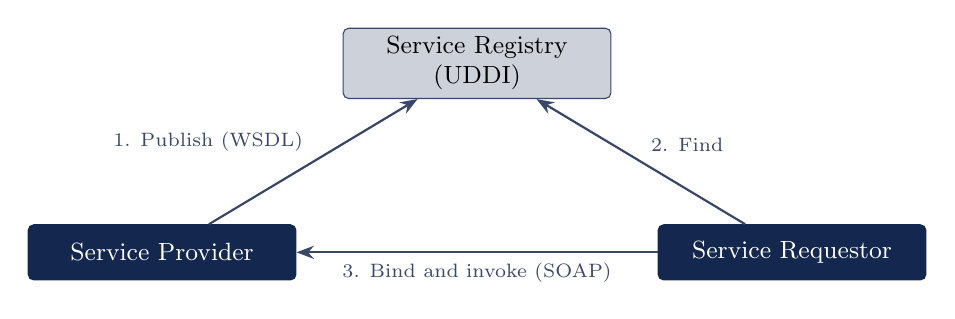
\begin{tikzpicture}
  \node[mid,minimum width=3.4cm] (reg) at (4,2.4) {Service Registry\\(UDDI)};
  \node[dark,minimum width=3.4cm] (prov) at (0,0) {Service Provider};
  \node[dark,minimum width=3.4cm] (req) at (8,0) {Service Requestor};
  \draw[arr] (prov) -- node[above left,font=\scriptsize] {1. Publish (WSDL)} (reg);
  \draw[arr] (req) -- node[above right,font=\scriptsize] {2. Find} (reg);
  \draw[arr] (req) -- node[below,font=\scriptsize] {3. Bind and invoke (SOAP)} (prov);
\end{tikzpicture}
\caption{The publish--find--bind triangle of SOA.}
\end{figure}

\begin{solved}{SOA interactions}
\Given Roles: service provider, registry, requestor.
\Formula Publish: provider $\to$ registry; Find: requestor $\to$ registry; Bind: requestor $\to$ provider.
\Steps
\begin{enumerate}[leftmargin=*]
  \item The provider describes the service in WSDL and publishes it to the registry.
  \item The requestor queries the registry and finds a suitable service.
  \item The requestor binds directly to the provider and invokes operations.
\end{enumerate}
\Answer Publish, Find, Bind as stated.
\end{solved}

\subsection{The Web Service Stack}
\begin{center}
\begin{tabularx}{\textwidth}{>{\bfseries}lX}
\toprule
Layer & Role\\
\midrule
XML & Uniform data format (derived from SGML); tags are user-defined; describes data, whereas HTML describes
display\\
SOAP & Simple Object Access Protocol: message format over Internet protocols\\
WSDL & Web Service Description Language: operations, messages, binding\\
UDDI & Universal Description, Discovery and Integration: registry\\
\bottomrule
\end{tabularx}
\end{center}

\textbf{SOAP building blocks:} Envelope (required; identifies the document as SOAP), Header (optional), Body (required;
call and response data), Fault (optional). Messages are request/response over HTTP (POST). SOAP is extensible, neutral
(any transport) and independent (any programming model). Usage models: RPC-like exchange and document-style messaging.
SOAP uses HTTP and can therefore use HTTPS for security; the WS-Security family adds message-level security.

\begin{lstlisting}[language=XML]
POST /InStock HTTP/1.1
Host: www.stock.org
Content-Type: application/soap+xml; charset=utf-8

<soap:Envelope xmlns:soap="http://www.w3.org/2003/05/soap-envelope">
  <soap:Body>
    <m:GetStockPrice xmlns:m="http://www.stock.org/stock">
      <m:StockName>IBM</m:StockName>
    </m:GetStockPrice>
  </soap:Body>
</soap:Envelope>
\end{lstlisting}

\textbf{WSDL document structure:} \texttt{types}, \texttt{message} (with \texttt{part}s), \texttt{portType} (operations),
\texttt{binding} and \texttt{service}. Example fragment: a message \texttt{getTermRequest} with part \texttt{term} of
type \texttt{xs:string}, and a response message \texttt{getTermResponse}.

\textbf{UDDI:} a framework to describe services, discover businesses and integrate business services; provides a service
registry supporting publish and find. Benefits: discovering the right business from millions online, defining how services
interact, and describing services and business processes programmatically.
The WS-* family (WS-Security, WS-Policy, WS-Trust, WS-Privacy, WS-SecureConversation, WS-Federation) extends SOAP.

\begin{solved}{What do traditional web services solve? (Assignment 2, Q7--Q9)}
\Given Candidate capabilities: HTTP/HTTPS firewall passage, cross-language interoperability, ultra-low-latency
real-time communication, UDDI discovery.
\Formula XML/SOAP overhead $\Rightarrow$ no ultra-low latency; WSDL names the interface; UDDI discovers.
\Steps
\begin{enumerate}[leftmargin=*]
  \item HTTP/HTTPS: addressed. XML/SOAP/WSDL interoperability: addressed. UDDI discovery: addressed.
  \item XML parsing and SOAP overhead add delay, so microsecond-level real-time messaging is \emph{not} addressed.
  \item The interface (operations, messages, binding) is described by \textbf{WSDL}; UDDI only registers and discovers.
\end{enumerate}
\Answer Items (i), (ii), (iv) addressed, (iii) not (Q9: B); WSDL describes the interface (Q7: B); SOAP provides (i), (ii),
(iii) (Q8: A).
\end{solved}

\subsection{Web Service Example: Web-based Purchase}
A purchase order service calls invoice and consolidation services; the workflow is composed through SOAP messages
discovered via a registry, illustrating loose coupling and platform independence.

\section{Week 2 Assignment Review}
\begin{center}
\begin{tabularx}{\textwidth}{cXc}
\toprule
Q & Concept tested & Answer\\
\midrule
1 & Hypercalls $\Rightarrow$ para-virtualization & C\\
2 & Full (hardware-assisted): unmodified guest, CPU extensions & B\\
3 & Public cloud: open use, owned by provider & B\\
4 & DOM for random access and modification & C\\
5 & Hypervisor / guest OS / host OS roles & B\\
6 & Hosted private cloud: SLA, compliance, latency all matter & D\\
7 & WSDL describes the web service interface & B\\
8 & SOAP: platform independence, XML, UDDI discovery & A\\
9 & Web services do not address ultra-low latency & B\\
10 & SOA publish--find--bind & A\\
\bottomrule
\end{tabularx}
\end{center}

% ==================================================================
%  WEEK 3
% ==================================================================
\chapter{SLAs, Cloud Economics, Data Management, MapReduce and OpenStack}

\section{Service Level Agreements (SLA)}
\begin{defbox}{Service Level Agreement}
A formal contract between a service provider and a consumer that specifies the services to be delivered,
the measurable level of service (Service Level Objectives), how it is monitored, and the remedies or penalties
when objectives are missed.
\end{defbox}

\textbf{SLA contents:} the set of services the provider will deliver; a complete, specific definition of each
service; responsibilities of provider and consumer; the efficiency/quality metrics; how performance is monitored,
audited and reported; the procedure for dispute resolution; and the consequences (credits, penalties) of
non-compliance, including how the SLA is changed or terminated.

\textbf{Web-service SLA:} \emph{WS-Agreement} is an XML-based language and protocol for negotiating, establishing and
managing agreements. \textbf{Cloud SLA versus web-service SLA:} traditional QoS parameters (response time,
throughput) are supplemented in the cloud by availability, resource capacity, scalability, elasticity and
provisioning-time parameters.

\textbf{Types of SLA:} \emph{off-the-shelf} (non-negotiable, standard terms of the provider) and \emph{negotiated}
(customised). \textbf{Multilevel SLA:} corporate level (applies to all customers), customer level (specific to a
customer) and service level (specific service).

\textbf{Service Level Objectives (SLOs)} are objectively measurable conditions for the service (for example
availability $\ge 99.9\%$, response time below 200~ms). \textbf{Service-level management} means monitoring and measuring
service performance against SLOs.

\textbf{Considerations for an SLA:} business-level objectives; responsibilities of provider and consumer;
business continuity and disaster recovery; maintenance; data location and portability; security controls;
regulatory compliance; and exit (termination) terms.

\textbf{Key Performance Indicators (KPIs):} low-level resource metrics (CPU, memory, bandwidth) are combined into
higher-level indicators; the questions are who should monitor (consumer, provider or third party) and how often.
\textbf{Metrics for monitoring and auditing:} throughput (how quickly the service responds), reliability, load balancing,
durability, elasticity, linearity, agility (how quickly the provider responds to change) and automation, performance
and cost metrics.

\textbf{Expected SLA parameters by model:} \emph{IaaS} -- CPU capacity, memory, storage, network, availability,
provisioning time; \emph{PaaS} -- integration, scalability, pay-as-you-go billing, environment; \emph{SaaS} --
reliability, usability, scalability, availability, customizability.

\textbf{Limitations:} service measurement is restricted to uptime percentage; measurement is often the customer's
burden; there is a gap between QoS hype and the SLA offerings in reality; credits are small compared with business
loss.

\subsection{Availability and Downtime}
\begin{thmbox}{Allowed downtime}
\[ \text{Allowed downtime} = (1 - A)\times T_{\text{service}}, \qquad
   A_{\text{achieved}} = \frac{T_{\text{service}} - T_{\text{outage}}}{T_{\text{service}}}. \]
$T_{\text{service}}$ is the agreed \emph{scheduled} service time, which may be less than 24 hours a day.
\end{thmbox}

\begin{solved}{99.9\% availability per 30-day month}
\Given $A = 99.9\%$, month $= 30 \times 24 = 720$ hours.
\Formula Allowed downtime $= (1 - A) \times T$.
\Steps
\begin{enumerate}[leftmargin=*]
  \item $1 - 0.999 = 0.001$.
  \item $0.001 \times 720 = 0.72$ hours.
  \item $0.72 \times 60 = 43.2$ minutes.
\end{enumerate}
\Answer About \textbf{0.72 hours} ($\approx 43$ minutes).
\end{solved}

\begin{solved}{Multilevel SLA conflict (Assignment 3, Q2, Q3)}
\Given Corporate level 95\%, customer level 98\%, service level 99.9\% uptime.
\Formula The most specific, most granular level governs accountability for the actual service.
\Steps
\begin{enumerate}[leftmargin=*]
  \item A multilevel SLA consists of all three levels: corporate, customer and service.
  \item In a conflict, the service-level SLA (99.9\%) is the binding, most specific commitment.
\end{enumerate}
\Answer Service-level SLA (Q3: C); a multilevel SLA includes (i), (ii) and (iii) (Q2: D).
\end{solved}

\begin{notebox}{What belongs in an SLA? (Assignment 3, Q1, Q4)}
RTO, MTTR, penalty/credit calculation and availability percentage are SLA items. The exact encryption algorithm and
key-storage procedure belong to security documents, not the SLA. Reliability and recoverability are quantified by
\textbf{availability} and \textbf{Mean Time To Recovery (MTTR)}.
\end{notebox}

\section{Cloud Economics}
Economic properties of the cloud:
\begin{itemize}[leftmargin=*]
  \item \textbf{Common infrastructure:} pooled standardized resources with benefits from statistical multiplexing.
  \item \textbf{Location independence:} ubiquitous availability with latency reduction and better user experience.
  \item \textbf{Online connectivity:} the enabler of other attributes.
  \item \textbf{Utility pricing:} pay-per-use, beneficial where demand varies.
  \item \textbf{On-demand resources:} elastic provisioning without delay or change cost.
\end{itemize}

\subsection{Value of Common Infrastructure: Statistics of Scale}
Multiplexing demand raises utilization and lowers cost per delivered resource. Smoothness is measured by the
\textbf{coefficient of variation}
\[ C_v = \frac{\sigma}{|\mu|}. \]
\begin{thmbox}{Aggregating independent demands}
For $n$ independent demands $X_1,\dots,X_n$ with identical mean $\mu$ and standard deviation $\sigma$:
mean $= n\mu$, variance $= n\sigma^2$, so
\[ C_v^{\text{agg}} = \frac{\sqrt{n}\,\sigma}{n\mu} = \frac{C_v}{\sqrt{n}}. \]
Perfectly correlated demands ($n X$) leave $C_v$ unchanged; negatively correlated demands ($X$ and $1-X$) smooth the sum
to a constant.
\end{thmbox}

\begin{solved}{Smoothing by aggregation}
\Given 100 independent workloads, each with $\mu = 40$ units and $\sigma = 20$ units.
\Formula $C_v = \sigma/\mu$; $C_v^{\text{agg}} = C_v/\sqrt{n}$.
\Steps
\begin{enumerate}[leftmargin=*]
  \item Single workload: $C_v = 20/40 = 0.5$.
  \item Aggregate: $C_v^{\text{agg}} = 0.5/\sqrt{100} = 0.5/10 = 0.05$.
  \item Check: mean $= 4000$, std $= \sqrt{100}\times 20 = 200$, $200/4000 = 0.05$.
\end{enumerate}
\Answer $C_v$ falls from 0.5 to 0.05: aggregating 100 workloads reduces the penalty to 10\%.
\end{solved}

\subsection{Value of Location Independence}
Latency depends strongly on distance and (second order) on routing; light in fibre covers only about 124 miles per
millisecond; human response latency is tens to hundreds of ms; VoIP with latency above about 200~ms degrades.
A global user base needs a dispersed architecture, raising coordination, consistency, availability and partition-tolerance issues.

\subsection{Value of Utility Pricing}
Cloud services need not be cheaper per unit to be economical: renting a car at INR 45,000 per day versus owning at INR 10,000 per day is
cheaper if you need it for only two days. Let $D(t)$ be demand for $0<t<T$, $P=\max D(t)$ the peak, $A=\operatorname{avg} D(t)$
the average, $B$ the baseline (owned) unit cost, $C$ the cloud unit cost, and $U = C/B$ the \emph{utility premium}.
\begin{align*}
 C_T &= U\,B\int_0^T D(t)\,dt = A\,U\,B\,T, &
 B_T &= P\,B\,T \quad(\text{baseline must handle peak}).
\end{align*}
\begin{thmbox}{When is the cloud cheaper?}
\[ C_T < B_T \iff U < \frac{P}{A}. \]
The cloud is cheaper when the utility premium is less than the ratio of peak to average demand.
\end{thmbox}

\begin{figure}[H]
\centering
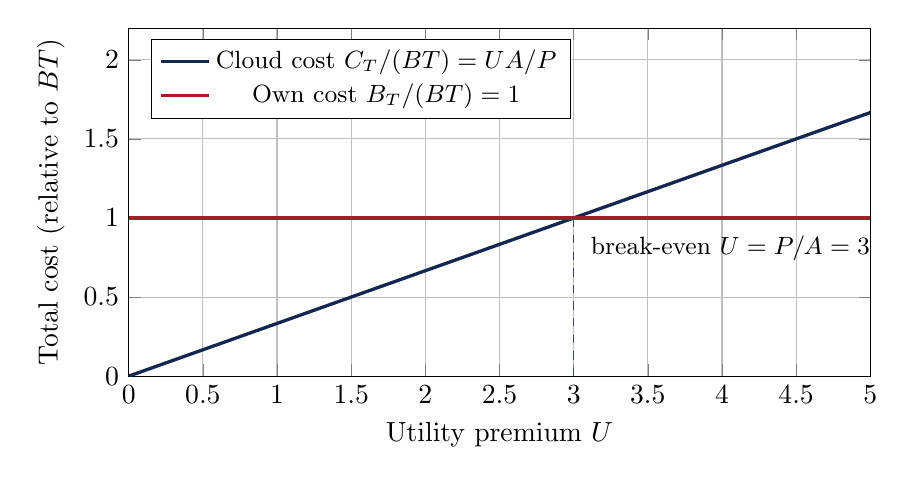
\begin{tikzpicture}
\begin{axis}[width=11cm,height=6cm,xlabel={Utility premium $U$},ylabel={Total cost (relative to $B T$)},
  xmin=0,xmax=5,ymin=0,ymax=2.2,legend pos=north west,legend style={font=\small},grid=major]
  \addplot[navy,very thick,domain=0:5] {x/3};
  \addplot[darkred,very thick,domain=0:5] {1};
  \draw[dashed,slate] (axis cs:3,0) -- (axis cs:3,1);
  \node[font=\small,anchor=north west] at (axis cs:3.05,0.95) {break-even $U=P/A=3$};
  \legend{Cloud cost $C_T/(BT)=U A/P$,Own cost $B_T/(BT)=1$}
\end{axis}
\end{tikzpicture}
\caption{Cloud versus owned cost for $P/A = 3$: break-even at $U = 3$.}
\end{figure}

\begin{solved}{Own or rent?}
\Given Average demand $A = 75$, peak demand $P = 225$, utility premium $U = 2.8$.
\Formula Cloud cheaper iff $U < P/A$.
\Steps
\begin{enumerate}[leftmargin=*]
  \item $P/A = 225/75 = 3$.
  \item $U = 2.8 < 3$.
\end{enumerate}
\Answer Cloud cost $<$ owning cost.
\end{solved}

\textbf{Real-world note:} demand is often spiky (promotions, tax season, flash crowds); a hybrid model is often best; network
cost, interoperability overhead, reliability and accessibility must also be considered.

\subsection{Value of On-demand Services and Penalty Cost}
Owned resources incur a penalty whenever resources $R(t)$ do not match demand $D(t)$:
$\text{Penalty} \propto \int |D(t) - R(t)|\,dt$. If demand is flat, the penalty is zero; for linear demand periodic provisioning is
acceptable; for exponential demand $D(t) = e^t$ with provisioning delay $t_p$, $R(t) = e^{t-t_p}$ and
$D - R = e^t(1 - e^{-t_p}) = k_1 e^t$, so the penalty grows exponentially.

\begin{solved}{Penalty with provisioning delay (tutorial Assignment 1)}
\Given Peak demand 120 units; $D(t) = 50\sin t$ for $0 \le t < \pi/2$ and $20\sin t$ for $\pi/2 \le t < \pi$;
$R(t) = D(t) + \delta\,\dfrac{dD}{dt}$ with $\delta = \pi/12$; unit cost 0.9.
\Formula Penalty $= 0.9 \int |D(t) - R(t)|\,dt = 0.9\,\delta \int |D'(t)|\,dt$.
\Steps
\begin{enumerate}[leftmargin=*]
  \item $D - R = -\delta D'(t)$, hence $|D - R| = \delta |D'(t)|$.
  \item On $[0,\pi/2)$: $D' = 50\cos t$, $\int_0^{\pi/2} 50\cos t\,dt = 50$.
  \item On $[\pi/2,\pi)$: $|D'| = 20|\cos t|$, $\int_{\pi/2}^{\pi} 20|\cos t|\,dt = 20$.
  \item Total $\int |D'|\,dt = 70$ (the jump at $t=\pi/2$ is treated as a single instant and ignored).
  \item Penalty $= 0.9 \times \dfrac{\pi}{12} \times 70 = 5.25\pi$.
\end{enumerate}
\Answer Penalty $\approx 16.5$ cost units; the provisioning delay makes the cloud under-supply on the rising part of demand and
over-supply on the falling part.
\end{solved}

\begin{solved}{Cloud versus owned for decaying demand (tutorial Assignment 2)}
\Given $D(t) = 50(1 + e^{-t})$, peak $P=100$ (at $t=0$), baseline unit cost $B = 120$, cloud unit cost $C = 200$, period $T = 100$.
\Formula $B_T = P\,B\,T$; $C_T = C\int_0^T D(t)\,dt$.
\Steps
\begin{enumerate}[leftmargin=*]
  \item $B_T = 100 \times 120 \times 100 = 1{,}200{,}000$.
  \item $\int_0^{100} 50(1 + e^{-t})\,dt = 50\,[\,100 + (1 - e^{-100})\,] \approx 5050$.
  \item $C_T = 200 \times 5050 = 1{,}010{,}000$.
  \item Cross-check: $A \approx 50.5$, $U = 200/120 = 1.67 < P/A = 100/50.5 = 1.98$.
\end{enumerate}
\Answer Yes, cloud cost $1.01\times10^6 <$ own cost $1.2\times10^6$.
\end{solved}

\section{Managing Data in the Cloud}
\subsection{Relational and Parallel Databases}
Relational databases are the default storage and retrieval mechanism, accessed through SQL by applications; the
database file-system layer provides indexing and transaction support. \textbf{Row-oriented storage} is optimal
for write-intensive transactional workloads; \textbf{column-oriented storage} is optimal for read-heavy analytics
(only needed columns are read, and similar values compress well).

\begin{center}
\begin{tabularx}{\textwidth}{>{\bfseries}lXX}
\toprule
Architecture & Description & Suitable for\\
\midrule
Shared memory & CPUs share one address space managed by an SMP operating system & Servers with multiple CPUs\\
Shared disk & Independent servers share storage over a high-speed network (NAS or SAN; Ethernet, Fibre Channel or Infiniband)
& Hybrid, moderate scale\\
Shared nothing & Cluster of independent servers each with own disk, connected by a network; tables partitioned across nodes &
Massively parallel, large scale\\
\bottomrule
\end{tabularx}
\end{center}
\textbf{Advantages of a parallel DB over a relational DB:} efficient SQL execution on multiple processors; partitioned tables with a
distributed-join optimizer; distributed two-phase commit locking; fault tolerance via stand-by systems.
Examples: Oracle, DB2, SQL Server (transaction processing); Netezza, Vertica, Teradata (data warehousing).
(Assignment 3, Q6: parallel DBs speed up analytics by \emph{distributed query execution across nodes}.)

\subsection{Google File System and HDFS}
GFS manages large files on a very large cluster of commodity servers. Failures must be tolerated because for $N$
components $p(\text{system failure}) = 1 - (1 - p)^N \to 1$ for large $N$.
\begin{itemize}[leftmargin=*]
  \item A single \textbf{Master} (GFS) / \textbf{NameNode} (HDFS) controls the namespace and metadata.
  \item Files are split into \textbf{chunks} (GFS) / \textbf{blocks} (HDFS) of typically 64~MB, stored on \textbf{chunk servers} /
        \textbf{data nodes}, replicated three times on different racks and network segments.
  \item \textbf{Read:} client sends path and offset to the master, gets replica metadata, caches it and reads from a chunk
        server.
  \item \textbf{Write/append:} master returns metadata for all replicas; client pushes data to all; the master designates a
        \emph{primary}, which chooses the offset, applies the append and tells replicas; on any failure the primary retries.
  \item \textbf{Fault tolerance:} heartbeat messages; metadata updated on failure; a new primary is assigned if the primary fails.
\end{itemize}

\begin{figure}[H]
\centering
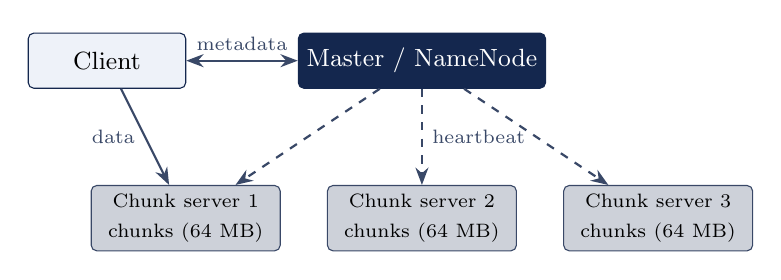
\begin{tikzpicture}
  \node[dark,minimum width=3cm] (m) at (4,2) {Master / NameNode};
  \node[box,minimum width=2cm] (cl) at (0,2) {Client};
  \foreach \xx/\nm in {1/{Chunk server 1},4/{Chunk server 2},7/{Chunk server 3}}{
    \node[mid,minimum width=2.4cm] (cs\xx) at (\xx,0) {\scriptsize \nm\\\scriptsize chunks (64 MB)};
  }
  \draw[darr] (cl)--(m) node[midway,above,font=\scriptsize] {metadata};
  \draw[arr] (cl)--(cs1) node[midway,left,font=\scriptsize] {data};
  \draw[arr,dashed] (m)--(cs4) node[midway,right,font=\scriptsize] {heartbeat};
  \draw[arr,dashed] (m)--(cs7);
  \draw[arr,dashed] (m)--(cs1);
\end{tikzpicture}
\caption{GFS/HDFS architecture: control path through the master, data path directly to chunk servers.}
\end{figure}

\begin{solved}{Chunks and failure probability}
\Given A 1 GB file, chunk size 64 MB, replication factor 3; component failure probability $p = 0.001$ in a system of $N = 1000$ components.
\Formula Chunks $= \lceil \text{size}/\text{chunk size} \rceil$; $p_{\text{sys}} = 1 - (1-p)^N$.
\Steps
\begin{enumerate}[leftmargin=*]
  \item $1024/64 = 16$ chunks; replicas $= 16 \times 3 = 48$ chunk copies.
  \item $p_{\text{sys}} = 1 - 0.999^{1000} = 1 - 0.3677 = 0.632$.
\end{enumerate}
\Answer 16 chunks (48 copies stored); with 1000 components some failure is likely ($\approx 63\%$), so fault tolerance is mandatory.
\end{solved}

\subsection{BigTable}
A distributed structured storage system built on GFS: a \textbf{sparse, persistent, multi-dimensional sorted map} indexed by
\emph{row key, column key and timestamp}. Columns are grouped into \emph{column families} (fixed at table creation, with labels
created dynamically as \texttt{family:label}); each cell keeps multiple versions in decreasing timestamp order. Tables split into
row ranges called \textbf{tablets}, each managed by a \textbf{tablet server}, stored as \emph{SSTable} files per column family; a
metadata table (with a root tablet) locates tablets. Supports large parallel reads and inserts; inserts are sorted and need more
work than a simple append.

\subsection{Dynamo}
Developed by Amazon for large volumes of concurrent small updates (key--value model, no dependence on GFS/HDFS), suited to
e-commerce.
\begin{itemize}[leftmargin=*]
  \item Objects are $\langle$key, value$\rangle$ pairs; \textbf{MD5} yields a 128-bit hash whose range maps to \emph{virtual nodes
        on a ring}; each physical node holds several virtual nodes. Objects replicate to $N$ nodes.
  \item Writes execute at a virtual node and are forwarded to replicas; load balancing handles transient failures and partitions.
  \item \textbf{Versioning with vector timestamps}: superseded versions are discarded; concurrent writes keep all versions, returned
        to readers for conflict resolution.
  \item \textbf{Quorum:} a read touches $R$ replicas, a write touches $W$; if $R + W > N$ the system is quorum consistent.
\end{itemize}

\begin{figure}[H]
\centering
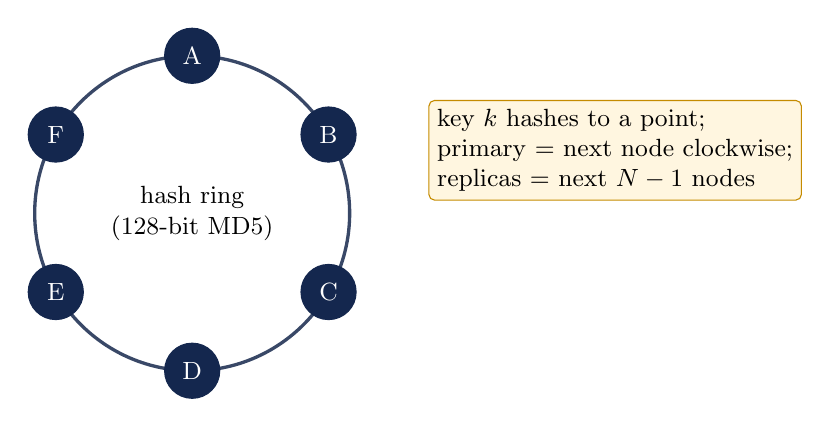
\begin{tikzpicture}
  \draw[slate,very thick] (0,0) circle (2cm);
  \foreach \ang/\nm in {90/A,30/B,330/C,270/D,210/E,150/F}{
    \node[dark,circle,inner sep=2pt,font=\small] (v\nm) at (\ang:2cm) {\nm};
  }
  \node[font=\small,align=center] at (0,0) {hash ring\\(128-bit MD5)};
  \node[gold,anchor=west,align=left,font=\small] at (3,0.8) {key $k$ hashes to a point;\\primary = next node clockwise;\\replicas = next $N-1$ nodes};
\end{tikzpicture}
\caption{Dynamo consistent-hashing ring with virtual nodes.}
\end{figure}

\begin{solved}{Quorum consistency}
\Given $N = 3$ replicas. Configurations: (a) $R=1, W=1$; (b) $R=2, W=2$; (c) $R=1, W=3$.
\Formula Quorum consistent iff $R + W > N$.
\Steps
\begin{enumerate}[leftmargin=*]
  \item (a) $1 + 1 = 2 \not> 3$: not consistent.
  \item (b) $2 + 2 = 4 > 3$: consistent.
  \item (c) $1 + 3 = 4 > 3$: consistent; reads are fast, writes slow.
\end{enumerate}
\Answer (b) and (c). Raising $W$ favours reads; raising $R$ favours writes.
\end{solved}

\subsection{Datastore (App Engine) and SimpleDB}
All entities reside in one BigTable table (single column family, no column-oriented storage), sharded and sorted lexicographically by
key. Entities are grouped by ancestry for transactions; \emph{prefix and range queries} are efficient. Index tables support queries:
automatically created \textbf{single-property} and \textbf{kind} indexes, and configurable \textbf{composite} indexes; the index
with highest selectivity is chosen.

\section{Introduction to MapReduce}
MapReduce is the programming model developed at Google for large-scale text processing and search on data in BigTable/GFS; it is
fault tolerant and runs on tens of thousands of processors. \emph{Hadoop} (Yahoo!) is the open-source implementation.

\subsection{Parallel Efficiency}
\[ \varepsilon = \frac{T_{1}}{p \cdot T_{p}} \]
where $T_1$ is the uniprocessor time and $T_p$ the time on $p$ processors. Inefficiencies arise from synchronization,
message overhead and load imbalance. An implementation is \emph{scalable} if efficiency stays constant when data and processors grow
proportionally.

\textbf{Illustration (word frequencies).} With $n$ documents, $m$ distinct words, each word occurring $f$ times per document on
average, read cost $c$ per word:
\begin{itemize}[leftmargin=*]
  \item Single processor: $n\,m\,f\,c$.
  \item \emph{Approach 1} (each processor handles $m/p$ words): every processor reads all words of all documents, $n\,(m/p)\,f$ useful
        reads but scans everything $\Rightarrow$ efficiency falls with $p$ (not scalable).
  \item \emph{Approach 2} (each processor handles $n/p$ documents for all $m$ words): reads $(n/p)\,m\,f\,c$, writes partial vector
        $c\,m$, merges $p\,(m/p)\,c$; every read is useful, efficiency tends to 1 as $n$ grows ($p \ll nf$).
\end{itemize}

\subsection{The Model}
\begin{figure}[H]
\centering
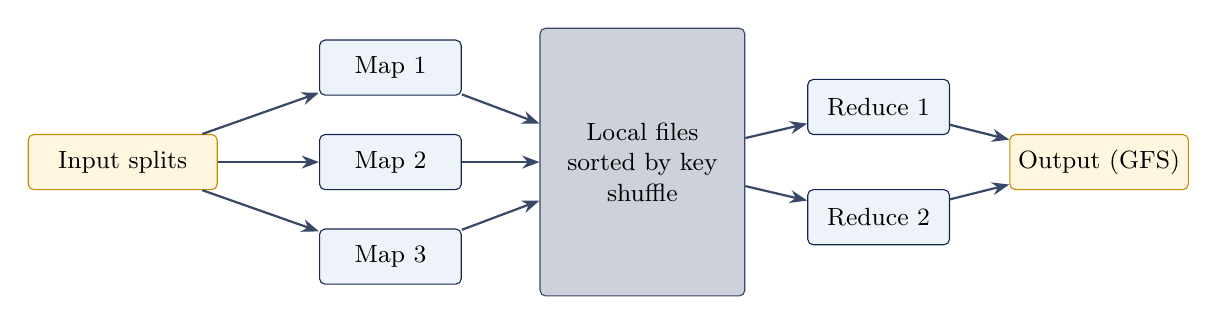
\begin{tikzpicture}[node distance=7mm]
  \node[gold,minimum width=2.4cm] (in) at (0,0) {Input splits};
  \foreach \i/\y in {1/1.2,2/0,3/-1.2}{
    \node[box,minimum width=1.8cm] (m\i) at (3.4,\y) {Map \i};
  }
  \node[mid,minimum width=2.6cm,minimum height=3.4cm] (sh) at (6.6,0) {Local files\\sorted by key\\shuffle};
  \foreach \i/\y in {1/0.7,2/-0.7}{
    \node[box,minimum width=1.8cm] (r\i) at (9.6,\y) {Reduce \i};
  }
  \node[gold,minimum width=1.8cm] (out) at (12.4,0) {Output (GFS)};
  \foreach \i in {1,2,3}{ \draw[arr] (in)--(m\i); \draw[arr] (m\i)--(sh); }
  \foreach \i in {1,2}{ \draw[arr] (sh)--(r\i); \draw[arr] (r\i)--(out); }
\end{tikzpicture}
\caption{MapReduce data flow with 3 mappers and 2 reducers.}
\end{figure}

\textbf{Map phase:} each of $M$ mappers reads about $1/M$ of the input; the map function transforms key-value pairs
$(k_1,v_1)\to[(k_2,v_2)]$; each mapper writes one file per reducer, sorted by key, to its \emph{local} file system, and the master tracks
locations. \textbf{Reduce phase:} the master tells reducers where the partial files are; reducers fetch them by remote procedure call,
group values by key, apply the reduce function $(k_2,[v_2])\to$ output, and write results to GFS.
\textbf{Fault tolerance:} heartbeats; tasks with no progress are duplicated; a failed \emph{mapper} must be re-executed because its output
is on local disk; a failed \emph{reducer} needs only its unfinished tasks re-run since completed output is already in GFS.

\begin{lstlisting}
map(String docId, String text):
    for each word w in text:
        EmitIntermediate(w, 1)

reduce(String word, Iterator counts):
    total = 0
    for each c in counts:
        total += c
    Emit(word, total)
\end{lstlisting}

\subsection{MapReduce Efficiency}
For a task on data volume $D$ with per-word cost $c$: uniprocessor time
$wD = cD + c\,m\,D + c\,r\,\sigma D + c\,\sigma\mu D$ (read, map, reduce, write). With $P$ processors the extra overhead is each mapper writing
$\sigma D/P$ locally and each reducer reading it remotely, so the overhead is $\dfrac{2c\sigma D}{P}$ in addition to $\dfrac{wD}{P}$.
\[ \varepsilon_{MR} = \frac{wD}{P\left(\dfrac{wD}{P} + \dfrac{2c\sigma D}{P}\right)} = \frac{1}{1 + \dfrac{2c\sigma}{w}}. \]

\begin{solved}{MapReduce parallel efficiency}
\Given $w = c(1 + m + r\sigma + \sigma\mu)$ with $m = 1$, $r = 1$, $\sigma = 1$, $\mu = 0.1$ (so $w = 3.1c$).
\Formula $\varepsilon_{MR} = 1/(1 + 2c\sigma/w)$.
\Steps
\begin{enumerate}[leftmargin=*]
  \item $2c\sigma/w = 2c/(3.1c) = 0.645$.
  \item $\varepsilon_{MR} = 1/1.645 = 0.608$.
\end{enumerate}
\Answer About 61\% efficiency; efficiency is independent of $P$ and $D$, so the implementation is scalable.
\end{solved}

\textbf{Applications:} indexing a document collection (map emits $(w_i, d_k)$; reduce builds $(w_i, [d_{i1},\dots,d_{im}])$); relational operations
(joins, group-by) at large scale with fault tolerance; word count.

\begin{solved}{Combiner and shuffle volume (Assignment 3, Q9; Assignment 5, Q4, Q6, Q7)}
\Given Word count of 2 TB with mapper output 1.5 TB, reducers run out of disk; HDFS block size 128 MB, input file 700 MB.
\Formula Number of map tasks $= \lceil \text{file size} / \text{block size} \rceil$.
\Steps
\begin{enumerate}[leftmargin=*]
  \item A \textbf{combiner} pre-aggregates mapper output locally (summing counts per word), shrinking 1.5 TB drastically before the shuffle; without it
        everything reaches the reducers and the merge exhausts disk space. Fix: configure the combiner.
  \item $\lceil 700/128 \rceil = \lceil 5.47 \rceil = 6$ blocks $\Rightarrow$ 6 map tasks.
  \item The \textbf{Partitioner} decides which reducer receives a key (hash-based by default).
  \item The Combiner is optional and may run zero, one or many times, so the algorithm must stay correct without it.
\end{enumerate}
\Answer Combiner (B); 6 map tasks (B); Partitioner (B); Combiner (C).
\end{solved}

\begin{solved}{Blocks, average and grouped salary (tutorial problems)}
\Given Block size 64 MB; files of 64 KB, 65 MB, 127 MB. Set $A = (10,20,30,40,50)$.
\Formula Blocks per file $=\lceil \text{size}/64\,\text{MB}\rceil$. Average $=\sum x / n$ computed with pairs $(\text{sum},\text{count})$.
\Steps
\begin{enumerate}[leftmargin=*]
  \item 64 KB $\to$ 1 block; 65 MB $\to \lceil 1.02\rceil = 2$; 127 MB $\to \lceil 1.98\rceil = 2$. Total $=5$ blocks.
  \item Mapper emits $(\text{``avg''}, (x,1))$ for each integer; combiner/reducer adds component-wise: sum $=150$, count $=5$.
  \item Reducer outputs $150/5 = 30$.
\end{enumerate}
\Answer 5 blocks; average $= 30$. (Note: averaging the \emph{averages} of partial results is incorrect; carry $(\text{sum},\text{count})$.)
\end{solved}

\begin{lstlisting}
// Salary statistics grouped by gender
map(line):                          // "Name, Gender, Salary"
    (name, g, s) = parse(line)
    Emit(g, (s, 1))
reduce(gender, values):
    total = 0; n = 0
    for (s, c) in values: total += s; n += c
    Emit(gender, (total, total / n))

// Word length categorisation
map(word):
    L = length(word)
    if L <= 2: Emit("tiny", 1)
    else if L <= 5: Emit("small", 1)
    else if L <= 9: Emit("medium", 1)
    else: Emit("big", 1)
reduce(category, counts): Emit(category, sum(counts))
\end{lstlisting}

\section{OpenStack}
OpenStack is a cloud operating system controlling large pools of compute, storage and networking resources in a data centre,
managed through a dashboard. Origin: a collaboration between NASA and Rackspace. It offers IaaS (VMs on demand, provisioning,
snapshotting, networking).

\begin{center}
\begin{tabularx}{\textwidth}{>{\bfseries}llX}
\toprule
Service & Project & Function\\
\midrule
Compute & Nova & Manages VM lifecycle on hypervisors (scheduling, spawning)\\
Networking & Neutron & Virtual networks, routers, DHCP, security groups, floating IPs; routes tenant traffic\\
Object storage & Swift & Scalable, redundant object (blob) store\\
Block storage & Cinder & Persistent block volumes independent of VM lifecycle\\
Identity & Keystone & Authentication, authorization, service catalog, tokens\\
Image service & Glance & Stores and retrieves VM disk images\\
Telemetry & Ceilometer & Metering and monitoring for billing\\
Dashboard & Horizon & Web UI for users and administrators\\
\bottomrule
\end{tabularx}
\end{center}

\textbf{Provisioning flow:} (1) the user logs in via Horizon and specifies VM parameters (name, flavor, keys, image); (2) Keystone
authenticates and returns an auth token reused for later API calls; (3) the Nova API publishes a request to the scheduler
(rpc cast); the \emph{Nova scheduler} filters and weighs hosts; (4) Nova compute driver talks to the hypervisor; Glance supplies the image,
Neutron allocates network ports and Cinder attaches volumes. \textbf{Ephemeral storage} persists only until the VM terminates; Cinder
volumes persist beyond it.

\begin{figure}[H]
\centering
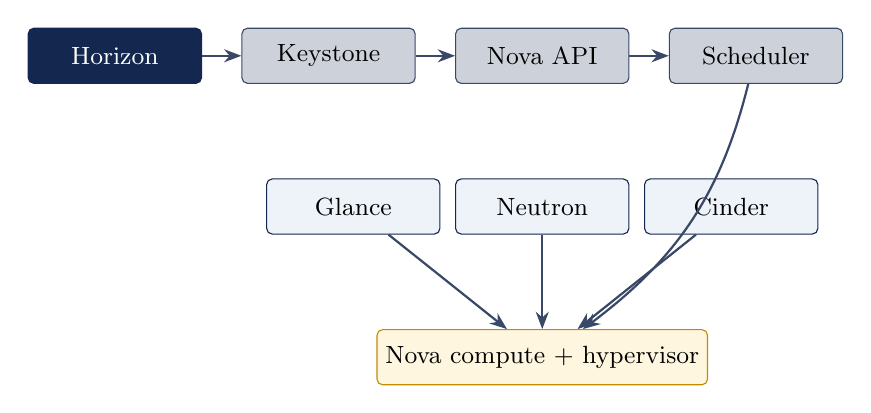
\begin{tikzpicture}[node distance=5mm]
  \node[dark,minimum width=2.2cm] (h) {Horizon};
  \node[mid,minimum width=2.2cm,right=of h] (k) {Keystone};
  \node[mid,minimum width=2.2cm,right=of k] (n) {Nova API};
  \node[mid,minimum width=2.2cm,right=of n] (s) {Scheduler};
  \node[box,minimum width=2.2cm,below=1.2cm of n,xshift=-2.4cm] (g) {Glance};
  \node[box,minimum width=2.2cm,below=1.2cm of n] (ne) {Neutron};
  \node[box,minimum width=2.2cm,below=1.2cm of n,xshift=2.4cm] (ci) {Cinder};
  \node[gold,minimum width=2.4cm,below=1.2cm of ne] (hy) {Nova compute + hypervisor};
  \draw[arr] (h)--(k); \draw[arr] (k)--(n); \draw[arr] (n)--(s);
  \draw[arr] (s) to[bend left=20] (hy);
  \draw[arr] (g)--(hy); \draw[arr] (ne)--(hy); \draw[arr] (ci)--(hy);
\end{tikzpicture}
\caption{Simplified OpenStack VM provisioning flow.}
\end{figure}

\begin{solved}{Over-subscription}
\Given A compute node with 640 physical vCPUs and a CPU allocation ratio of 5:1.
\Formula Allocatable vCPUs $=$ physical vCPUs $\times$ allocation ratio.
\Steps
\begin{enumerate}[leftmargin=*]
  \item $640 \times 5 = 3200$.
\end{enumerate}
\Answer 3200 virtual CPUs.
\end{solved}

\section{Week 3 Assignment Review}
\begin{center}
\begin{tabularx}{\textwidth}{cXc}
\toprule
Q & Concept tested & Answer\\
\midrule
1 & Items not in an SLA: encryption algorithm details & B\\
2 & Multilevel SLA: corporate, customer, service & D\\
3 & Service-level SLA binds in conflict & C\\
4 & Availability and MTTR & A\\
5 & 99.9\% of 720 h $\Rightarrow$ 0.72 h & A\\
6 & Parallel DB: distributed query execution & B\\
7 & Sub-second fraud detection: nightly batch is least suitable & C\\
8 & Petabyte imagery for Spark: object storage & B\\
9 & Missing combiner exhausts reducer disk & B\\
10 & $640 \times 5 = 3200$ vCPUs & B\\
\bottomrule
\end{tabularx}
\end{center}

% ==================================================================
%  WEEK 4
% ==================================================================
\chapter{Private Cloud with OpenStack, Microsoft Azure, and Google Cloud Platform}

\section{Introduction and Week Overview}
Week 4 bridges the theoretical foundations of virtualization and service-oriented architectures into concrete, production-grade cloud implementations. The curriculum covers three distinct cloud ecosystems:
\begin{enumerate}[leftmargin=*]
  \item \textbf{Private Cloud Implementation via OpenStack:} An empirical examination of IIT Kharagpur's on-premises cloud infrastructure (\emph{Meghamala}), exploring control plane components, hypervisor virtualization, and virtual machine lifecycle orchestration.
  \item \textbf{Microsoft Azure Ecosystem:} Enterprise infrastructure components, geographic resilience architectures (Regions and Availability Zones), Azure App Service deployment topologies, deployment slot mechanics, and scalable database decoupling (Azure SQL Database Hyperscale).
  \item \textbf{Google Cloud Platform (GCP):} Google's global network fabric, Platform-as-a-Service orchestration with Google App Engine (GAE), managed storage services, globally scalable relational consistency via Cloud Spanner, and real-time big data analytical pipelines.
\end{enumerate}

\section{Private Cloud Implementation: Meghamala at IIT Kharagpur}
\subsection{Architectural Blueprint and Infrastructure Topology}
\emph{Meghamala} (meaning ``Garland of Clouds'' in Sanskrit) is the dedicated private cloud computing facility at the Department of Computer Science and Engineering, IIT Kharagpur. Built on the open-source OpenStack platform, Meghamala serves institutional researchers, laboratory computing classes, and faculty development clusters.

The underlying infrastructure consists of high-density commodity server racks partitioned into:
\begin{itemize}[leftmargin=*]
  \item \textbf{Controller Nodes:} Running the OpenStack API daemons, message queue brokers (RabbitMQ), relational database instances (MariaDB/MySQL), and state coordination engines.
  \item \textbf{Network Nodes:} Executing OpenStack Neutron agents, virtual software switches (Open vSwitch / Linux Bridge), L3 routing daemons, DHCP agents, and metadata proxies.
  \item \textbf{Compute Nodes:} Running standard hypervisors (predominantly Linux KVM managed by \texttt{libvirt}) orchestrated by the \texttt{nova-compute} daemon, executing multi-tenant guest operating systems.
  \item \textbf{Storage Nodes:} Dedicated storage appliances hosting block storage pools (Cinder volumes backed by LVM, Ceph, or iSCSI SAN) and object storage clusters (Swift).
\end{itemize}

\begin{figure}[H]
\centering
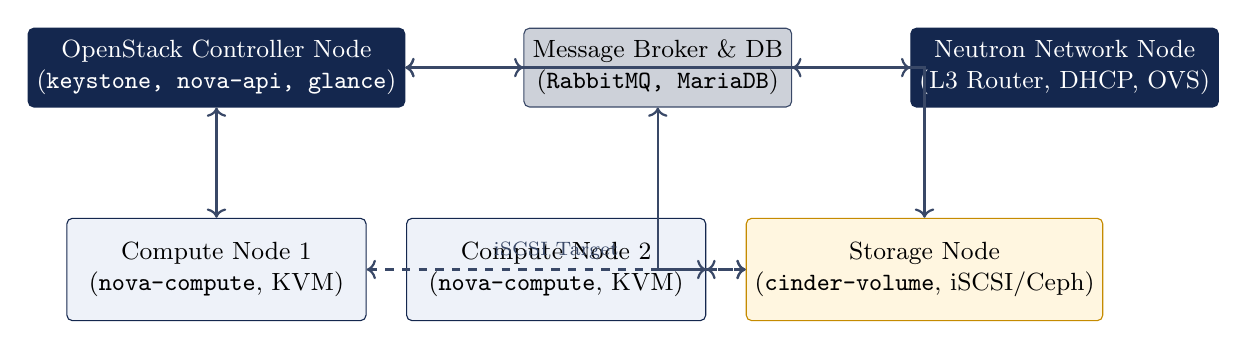
\begin{tikzpicture}[node distance=5mm, font=\small]
  % Controller Box
  \node[dark, minimum width=3.8cm, minimum height=1cm] (ctrl) {OpenStack Controller Node\\(\texttt{keystone, nova-api, glance})};
  \node[mid, right=1.5cm of ctrl, minimum width=3.4cm, minimum height=1cm] (msg) {Message Broker \& DB\\(\texttt{RabbitMQ, MariaDB})};
  \node[dark, right=1.5cm of msg, minimum width=3.4cm, minimum height=1cm] (net) {Neutron Network Node\\(L3 Router, DHCP, OVS)};

  % Compute and Storage
  \node[box, below=1.4cm of ctrl, minimum width=3.8cm, minimum height=1.3cm] (comp1) {Compute Node 1\\(\texttt{nova-compute}, KVM)};
  \node[box, right=0.5cm of comp1, minimum width=3.8cm, minimum height=1.3cm] (comp2) {Compute Node 2\\(\texttt{nova-compute}, KVM)};
  \node[gold, right=0.5cm of comp2, minimum width=3.8cm, minimum height=1.3cm] (cinder) {Storage Node\\(\texttt{cinder-volume}, iSCSI/Ceph)};

  % Interconnects
  \draw[arr, <->] (ctrl) -- (msg);
  \draw[arr, <->] (msg) -- (net);
  \draw[arr, <->] (ctrl) -- (comp1);
  \draw[arr, <->] (msg) |- (comp2);
  \draw[arr, <->] (ctrl) -| (cinder);
  \draw[arr, dashed, <->] (comp1) -- (cinder) node[midway, above, font=\scriptsize] {iSCSI Target};
  \draw[arr, dashed, <->] (comp2) -- (cinder);
\end{tikzpicture}
\caption{Meghamala OpenStack Physical and Logical Architecture.}
\end{figure}

\subsection{Horizon Web Dashboard: Operational Modules}
The primary administrative interface demonstrated in the lecture is OpenStack \textbf{Horizon}. The dashboard organizes cloud administrative actions into modular panels:

\begin{center}
\begin{tabularx}{\textwidth}{>{\bfseries}l p{3.2cm} X}
\toprule
Horizon Module & Corresponding Service & Demonstrated Operational Capabilities\\
\midrule
Project Overview & Horizon / Ceilometer & Graphical quota visualization (vCPUs allocated, RAM utilized, Floating IPs reserved, Security Group quotas).\\
Instances & Nova & Tabular listing of active, paused, or suspended VMs; display of hypervisor host, power state, task status, fixed IP (e.g., \texttt{10.4.0.x}), and public floating IP (e.g., \texttt{192.164.0.x}).\\
Flavors & Nova & Hardware profile templates defining virtual machine dimensions (e.g., \texttt{m1.tiny}: 1 vCPU, 512 MB RAM, 1 GB disk; \texttt{m1.large}: 4 vCPU, 8 GB RAM, 80 GB disk).\\
Images & Glance & Catalog of curated OS disk templates (Ubuntu Server, CentOS, Debian, CirrOS) uploaded in QCOW2 or RAW formats.\\
Volumes & Cinder & Lifecycle management of persistent block storage volumes; snapshot creation, volume expansion, and volume attachment to active Nova instances.\\
Networks \& Routers & Neutron & Software-defined virtual tenant networks (VXLAN/GRE overlays), internal subnet allocation, default gateway assignment, external network routing, and floating IP allocation pools.\\
Security Groups & Neutron & Stateful virtual firewalls operating at the port level; protocol, port range, and ingress/egress CIDR rule definition.\\
Access \& Security & Keystone / Nova & SSH key-pair generation, API access endpoints, and user credential tokens.\\
\bottomrule
\end{tabularx}
\end{center}

\subsection{Step-by-Step VM Provisioning and Access Workflow}
The demonstration shows the complete lifecycle of provisioning a virtual compute instance (named \texttt{cloud-nptel}) and establishing secure remote connectivity:

\begin{enumerate}[leftmargin=*]
  \item \textbf{Authentication and Scoping:} The user accesses Horizon via Web browser. Credentials (username and password) are sent to \textbf{Keystone}, which validates the user against the SQL identity backend and returns an unscoped token, followed by a scoped token associated with the specific tenant/project.
  \item \textbf{Instance Parameter Specification:}
    \begin{itemize}
      \item \emph{Instance Name:} \texttt{cloud-nptel}.
      \item \emph{Source:} Boot from Glance image (e.g., Ubuntu Linux LTS \texttt{.qcow2}).
      \item \emph{Flavor Selection:} Selection of computing capacity matching computational requirements.
      \item \emph{Network Attachment:} Binding the virtual network interface card (vNIC) to the tenant's private subnet (\texttt{10.4.0.0/24}).
      \item \emph{Security Group Assignment:} Enforcing ingress security rules: Port 22 (SSH) and custom remote desktop ports.
      \item \emph{Key Pair Association:} Injecting the user's public SSH key into the VM's \texttt{authorized\_keys} file via \texttt{cloud-init} during boot.
    \end{itemize}
  \item \textbf{Compute Node Scheduling:} The \texttt{nova-scheduler} applies filtering algorithms (checking available vCPUs, memory, and hypervisor architecture) and weighting algorithms to select the optimal physical compute node.
  \item \textbf{Image Caching and Hypervisor Execution:} The local \texttt{nova-compute} daemon fetches the base image from Glance, caches it locally, constructs an ephemeral copy-on-write overlay, writes the domain XML definition for \texttt{libvirt}, and boots the KVM guest.
  \item \textbf{Floating IP Association:} The instance initially receives an internal, non-routable private IP (\texttt{10.4.0.4}). To make the instance accessible from campus desktop workstations, a public floating IP (\texttt{192.164.0.8}) is allocated from the external pool and mapped via 1:1 NAT in the Neutron virtual router.
  \item \textbf{Remote Client Connectivity:}
    \begin{itemize}
      \item \emph{Command Line Access:} Direct terminal connection via secure shell:
      \begin{lstlisting}[language=bash]
ssh -i ~/.ssh/meghamala_key.pem ubuntu@192.164.0.8
      \end{lstlisting}
      \item \emph{Graphical Desktop Access via X2Go:} X2Go is an open-source remote desktop client based on NX technology, allowing high-performance graphical desktop access over low-bandwidth wide-area connections. The user configures an X2Go session targeting host \texttt{192.164.0.8}, specifying user \texttt{ubuntu}, RSA private key authentication, and session environment (e.g., XFCE or MATE).
    \end{itemize}
  \item \textbf{Instance Termination and Resource Reclamation:} When work completes, the user terminates the instance via Horizon. Nova signals \texttt{libvirt} to shut down the KVM process, deletes the ephemeral root disk, reclaims allocated RAM and vCPUs, and releases the private IP back to the Neutron DHCP pool. Associated Cinder volumes remain intact unless explicitly flagged for deletion.
\end{enumerate}

\begin{defbox}{Floating IP vs Fixed Private IP in OpenStack}
\textbf{Fixed IP:} An internal, tenant-private IP address automatically assigned by Neutron DHCP upon VM creation (e.g., \texttt{10.4.0.x}). It enables communication between instances within the same virtual network but is unreachable from outside the cloud.\\
\textbf{Floating IP:} A public, globally routable IP address (e.g., \texttt{192.164.0.x}) drawn from an external network allocation pool. It is dynamically bound to an instance's virtual interface via Network Address Translation (1:1 NAT) on the virtual router, enabling direct inbound and outbound WAN communication.
\end{defbox}

\section{Microsoft Azure Enterprise Architecture}
\subsection{Global Infrastructure: Regions and Availability Zones}
Microsoft Azure organizes physical infrastructure hierarchically to provide enterprise-grade reliability and legal compliance:
\begin{itemize}[leftmargin=*]
  \item \textbf{Data Center:} A physical building housing server racks, uninterruptible power supplies (UPS), cooling infrastructure, and network switches.
  \item \textbf{Availability Zone (AZ):} A physically separated location within a single Azure region. Each Availability Zone comprises one or more data centers equipped with independent power, cooling, and networking infrastructure. AZs are connected through high-speed, ultra-low-latency private fiber networks ($< 2\text{ ms}$ round-trip latency).
  \item \textbf{Region:} A defined geographical perimeter containing multiple Availability Zones (typically three or more). Examples include \emph{Central India}, \emph{East US}, and \emph{West Europe}.
  \item \textbf{Region Pairs:} Each Azure region is paired with another region within the same geography (at least 300 miles apart) to ensure business continuity during catastrophic disasters (e.g., hurricanes or regional power outages). Planned Azure platform updates are rolled out to paired regions sequentially to prevent concurrent platform downtime.
\end{itemize}

\begin{thmbox}{Availability Zone Fault Isolation Principle}
If two Virtual Machines or database instances are deployed across separate Availability Zones within the same Azure Region:
\begin{equation}
P(\text{Simultaneous Hardware Failure}) = P(\text{AZ}_1\text{ Failure}) \times P(\text{AZ}_2\text{ Failure}) \approx 0
\end{equation}
A catastrophic physical event (e.g., total utility power grid failure or flooding) disabling $\text{AZ}_1$ leaves $\text{AZ}_2$ entirely unaffected because power feeds, generator fuel supplies, chiller plants, and network carriers are physically independent.
\end{thmbox}

\subsection{Azure Resource Management Hierarchy}
Azure employs a strict hierarchical management model enforced through \textbf{Azure Resource Manager (ARM)}:
\begin{enumerate}[leftmargin=*]
  \item \textbf{Management Groups:} Containers that help manage access, policy, and compliance across multiple subscriptions.
  \item \textbf{Subscriptions:} Agreements with Microsoft that associate resource usage with billing accounts and govern resource quotas.
  \item \textbf{Resource Groups:} Logical containers into which Azure resources (web apps, virtual networks, storage accounts, databases) are deployed, managed, and monitored as a unified lifecycle unit. Deleting a resource group deletes all resources contained within it.
  \item \textbf{Resources:} Individual instances of cloud services (e.g., a virtual machine, virtual network, or database).
\end{enumerate}

\subsection{Azure App Service: Architecture and Deployment Topologies}
Azure App Service is a fully managed Platform-as-a-Service (PaaS) engine designed for hosting web applications, RESTful APIs, and mobile backends.

\subsubsection{App Service Plans}
An \textbf{App Service Plan} represents the set of compute resources allocated to run web apps. Every web application running in App Service must be associated with an active App Service Plan. Multiple applications can share a single App Service Plan to optimize cost.
\begin{center}
\begin{tabularx}{\textwidth}{>{\bfseries}l p{2.2cm} p{2.5cm} X}
\toprule
Pricing Tier & Scale Limits & Deployment Slots & Intended Enterprise Use Case\\
\midrule
Free / Shared & Shared CPU & None (0) & Prototyping, testing, and student projects.\\
Basic & Up to 3 dedicated VMs & None (0) & Low-traffic production workloads without automated scaling.\\
Standard & Up to 10 dedicated VMs & Up to 5 slots & Production workloads requiring auto-scaling, daily backups, and staging slots.\\
Premium (P1v3--P3v3) & Up to 30 dedicated VMs & Up to 20 slots & High-performance enterprise workloads, intense traffic, VNet integration, and maximum deployment slots.\\
Isolated & Up to 100 dedicated VMs & Up to 20 slots & Mission-critical workloads requiring dedicated hardware inside a private virtual network (App Service Environment).\\
\bottomrule
\end{tabularx}
\end{center}

\subsubsection{Deployment Slots Mechanics and Zero-Downtime Swaps}
Deployment slots are live web applications with their own distinct hostnames (e.g., \texttt{app-staging.azurewebsites.net} alongside \texttt{app.azurewebsites.net}). When a new build is deployed:
\begin{enumerate}[leftmargin=*]
  \item The application code is deployed to the \emph{staging} slot.
  \item Validation, warm-up requests, and automated regression tests run against staging without impacting live production traffic.
  \item A \textbf{Slot Swap} is triggered. The Azure routing subsystem swaps the virtual IP addresses and DNS bindings of the two slots. Traffic seamlessly flows to the newly warmed-up code with zero downtime.
  \item If an unforeseen bug emerges in production, an instantaneous reverse swap rolls back the environment immediately.
\end{enumerate}

\subsubsection{Security Configuration: HTTPS Only}
By default, web apps created in Azure accept plain HTTP traffic on port 80. Enabling the \textbf{HTTPS Only} setting activates an automated server-side HTTP 301 Permanent Redirect rule, routing all incoming unencrypted requests to encrypted HTTPS on port 443 with TLS certificates.

\subsection{Azure SQL Database: Decoupled Storage and Hyperscale Tier}
Traditional relational database management systems bind computing power (CPU and memory) tightly to physical disk arrays. Under heavy scaling, expanding storage requires database migration or extensive downtime.

\textbf{Azure SQL Database Hyperscale} revolutionizes relational storage by introducing a fully decoupled, cloud-native architecture:
\begin{itemize}[leftmargin=*]
  \item \textbf{Compute Tier:} Stateless compute nodes executing the SQL engine (query optimization, parsing, transaction coordinator). Compute nodes can scale up or down in seconds independently of data size. Read-only replicas can be added dynamically to scale read queries.
  \item \textbf{Page Servers:} Distributed secondary storage nodes that cache database pages in local solid-state drives (SSD) and serve read operations.
  \item \textbf{Log Service:} High-throughput, low-latency transaction log processing tier using Paxos consensus algorithms for deterministic durability.
  \item \textbf{Azure Storage Fabric:} Persistent long-term storage backed by Azure Blob Storage, allowing automatic storage expansion up to \textbf{100 TB} without application downtime or performance degradation.
\end{itemize}

\begin{figure}[H]
\centering
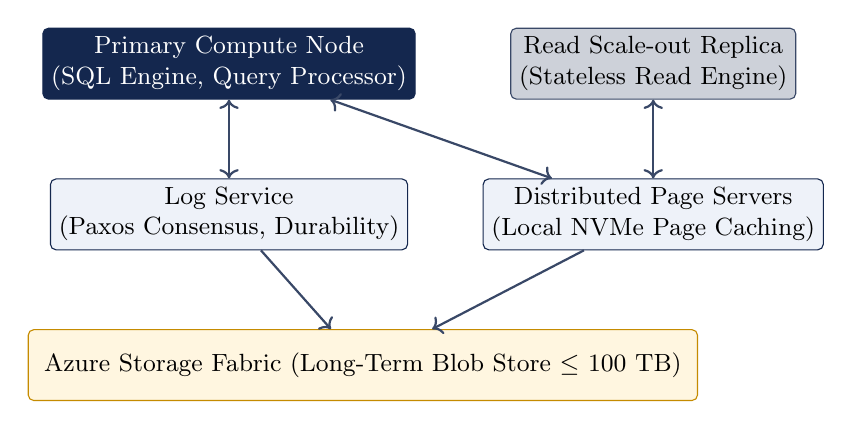
\begin{tikzpicture}[node distance=6mm, font=\small]
  \node[dark, minimum width=4cm, minimum height=0.9cm] (comp) {Primary Compute Node\\(SQL Engine, Query Processor)};
  \node[mid, right=1.2cm of comp, minimum width=3.2cm, minimum height=0.9cm] (replica) {Read Scale-out Replica\\(Stateless Read Engine)};

  \node[box, below=1cm of comp, minimum width=4cm, minimum height=0.9cm] (log) {Log Service\\(Paxos Consensus, Durability)};
  \node[box, below=1cm of replica, minimum width=3.8cm, minimum height=0.9cm] (page) {Distributed Page Servers\\(Local NVMe Page Caching)};

  \node[gold, below=1cm of log, minimum width=8.5cm, minimum height=0.9cm, xshift=1.7cm] (blob) {Azure Storage Fabric (Long-Term Blob Store $\le$ 100 TB)};

  \draw[arr, <->] (comp) -- (log);
  \draw[arr, <->] (comp) -- (page);
  \draw[arr, <->] (replica) -- (page);
  \draw[arr, ->] (log) -- (blob);
  \draw[arr, ->] (page) -- (blob);
\end{tikzpicture}
\caption{Azure SQL Database Hyperscale Decoupled Compute-Storage Architecture.}
\end{figure}

\subsection{Hands-On Deployment: Python Web App via Azure CLI}
The lecture demonstrates deploying a Python Flask application to Azure App Service using the Azure Cloud Shell:
\begin{lstlisting}[language=bash]
# Step 1: Clone the Flask starter template
git clone https://github.com/Azure-Samples/python-docs-hello-world
cd python-docs-hello-world

# Step 2: Configure deployment credentials for Git/FTP
az webapp deployment user set --user-name devadmin --password "SecretPassword123!"

# Step 3: Create an Azure Resource Group
az group create --name CloudNPTEL-RG --location "West Europe"

# Step 4: Provision an App Service Plan (Free SKU)
az appservice plan create --name NPTEL-ServicePlan \
   --resource-group CloudNPTEL-RG --sku FREE --is-linux

# Step 5: Provision the Web App container with Python 3.9 runtime
az webapp create --name nptel-demo-web-2024 \
   --resource-group CloudNPTEL-RG \
   --plan NPTEL-ServicePlan --runtime "PYTHON:3.9"

# Step 6: Configure local Git deployment endpoint
az webapp deployment source config-local-git \
   --name nptel-demo-web-2024 --resource-group CloudNPTEL-RG

# Step 7: Push source code to the remote Azure Git repository
git remote add azure https://devadmin@nptel-demo-web-2024.scm.azurewebsites.net/nptel-demo-web-2024.git
git push azure master
\end{lstlisting}

\section{Google Cloud Platform (GCP) Core Ecosystem}
\subsection{Google Global Infrastructure and Software-Defined Networking}
Google Cloud Platform runs on the identical physical infrastructure that powers Google Search, YouTube, and Gmail. Key differentiators highlighted in the curriculum include:
\begin{itemize}[leftmargin=*]
  \item \textbf{Global Private Fiber Network:} Traffic between GCP regions travels across Google's private transoceanic fiber backbone rather than the public Internet, dramatically reducing latency, jitter, and packet loss.
  \item \textbf{Andromeda SDN:} Google's custom software-defined network virtualization stack delivering high packet processing rates and massive bandwidth.
  \item \textbf{Jupiter Data Center Fabric:} Non-blocking bisection switching fabric delivering petabits-per-second aggregate bandwidth within data center clusters.
\end{itemize}

\subsection{Taxonomy of GCP Compute Services}
GCP provides a spectrum of compute abstractions spanning from bare hardware control to fully managed serverless execution:
\begin{center}
\begin{tabularx}{\textwidth}{>{\bfseries}l p{2.2cm} p{2.5cm} X}
\toprule
Compute Service & Model & Control Level & Core Technical Characteristic\\
\midrule
Compute Engine (GCE) & IaaS & Full OS / Kernel & Raw virtual machines; custom CPU/RAM configurations; local SSD scratch disks; live migration support.\\
Google Kubernetes Engine (GKE) & Managed PaaS / CaaS & Container Cluster & Enterprise managed Kubernetes; automated node repair, rolling upgrades, and horizontal pod autoscaling.\\
Cloud Run & Serverless CaaS & Container Image & Fully managed serverless container platform; scales down to zero instances; billed per 100 ms of CPU execution.\\
App Engine (GAE) & PaaS & Application Code & Turnkey application hosting; automatic traffic splitting, built-in load balancing, and automated zero-management scaling.\\
Cloud Functions & FaaS & Single Function & Event-driven code snippets executed in response to Cloud Storage, Pub/Sub, or HTTP webhook triggers.\\
\bottomrule
\end{tabularx}
\end{center}

\subsection{Google App Engine (GAE): Standard vs Flexible Environments}
Google App Engine provides two architectural runtimes:
\begin{itemize}[leftmargin=*]
  \item \textbf{Standard Environment:} Applications run in secure sandboxed language runtimes (Python, Java, Go, PHP, Node.js). It provides instantaneous scale-up in response to sudden traffic spikes and scales down to \textbf{zero instances} when traffic ceases, minimizing operational costs. However, it restricts background threads, filesystem writes, and custom OS packages.
  \item \textbf{Flexible Environment:} Applications execute inside Docker containers on managed Compute Engine virtual machines. It allows custom runtimes, background threads, and arbitrary C-extensions, but scaling takes several minutes and cannot scale to zero instances.
\end{itemize}

\subsubsection{Configuration and Deployment Mechanics}
An App Engine application is configured via \texttt{app.yaml}:
\begin{lstlisting}[language=bash]
# Minimal app.yaml for Python Flask on App Engine Standard
runtime: python39
instance_class: F1

handlers:
  - url: /static
    static_dir: static
  - url: /.*
    script: auto
\end{lstlisting}

Deployment and traffic orchestration commands:
\begin{lstlisting}[language=bash]
# Start local development server watching for file changes
dev_appserver.py app.yaml

# Deploy application to GCP App Engine
gcloud app deploy app.yaml --project gcp-nptel-cloud

# View running web application in default browser
gcloud app browse

# Split traffic between version v1 and version v2 (A/B testing)
gcloud app services set-traffic default --splits v1=0.8,v2=0.2
\end{lstlisting}

\subsection{GCP Storage and Database Services}
\begin{itemize}[leftmargin=*]
  \item \textbf{Cloud Storage (GCS):} Unified object storage offering four storage classes (Standard, Nearline, Coldline, Archive) accessible via HTTP REST APIs. It supports static website hosting by uploading HTML/CSS assets to a globally unique bucket, setting public read permissions (\texttt{allUsers:R}), and configuring default index (\texttt{index.html}) and 404 error pages.
  \item \textbf{Cloud SQL:} Fully managed relational database service supporting MySQL, PostgreSQL, and Microsoft SQL Server. It handles automated backups, read replicas, and vertical hardware scaling.
  \item \textbf{Cloud Spanner:} A globally distributed, enterprise relational database service that uniquely combines SQL semantics, horizontal scaling across continents, and \textbf{external consistency} (the strongest consistency guarantee in distributed systems) using synchronized hardware atomic clocks and GPS receivers (\textbf{TrueTime API}).
  \item \textbf{Firestore / Datastore:} Serverless, horizontally scalable NoSQL document database designed for mobile and web backends, supporting offline synchronization and ACID transactions.
  \item \textbf{BigQuery:} Serverless, highly scalable, petabyte-scale cloud data warehouse designed for fast SQL queries on massive datasets using Google's columnar storage format (Capacitor) and distributed execution engine (Dremel).
\end{itemize}

\section{Cross-Cloud Platform Comparative Matrix}
The following comparative table synthesizes equivalent service abstractions across the three leading public hyperscalers and the private OpenStack framework:

\begin{center}
\begin{tabularx}{\textwidth}{>{\bfseries}l l l l l}
\toprule
Functional Category & OpenStack & Microsoft Azure & Google Cloud (GCP) & Amazon Web Services (AWS)\\
\midrule
Compute (VMs) & Nova & Virtual Machines & Compute Engine (GCE) & Elastic Compute Cloud (EC2)\\
Containers (K8s) & Magnum & Azure Kubernetes (AKS) & Google Kubernetes (GKE) & Elastic Kubernetes (EKS)\\
Serverless PaaS & Solum & App Service & App Engine (GAE) & Elastic Beanstalk\\
Serverless FaaS & Qinling & Azure Functions & Cloud Functions & AWS Lambda\\
Block Storage & Cinder & Azure Managed Disks & Persistent Disk & Elastic Block Store (EBS)\\
Object Storage & Swift & Azure Blob Storage & Cloud Storage (GCS) & Simple Storage Service (S3)\\
Virtual Networking & Neutron & Azure Virtual Network & Virtual Private Cloud (VPC) & Virtual Private Cloud (VPC)\\
Identity \& IAM & Keystone & Azure Active Directory & Cloud IAM & AWS IAM\\
Relational SQL & Trove & Azure SQL Database & Cloud SQL / Spanner & Amazon RDS / Aurora\\
Data Warehouse & --- & Azure Synapse Analytics & BigQuery & Amazon Redshift\\
Message Bus & Zaqar & Azure Service Bus & Cloud Pub/Sub & Amazon SQS / SNS\\
\bottomrule
\end{tabularx}
\end{center}

\section{Comprehensive Solved Assignment Problems (Week 4)}

\begin{solved}{Azure SQL Database Hyperscale Storage Decoupling}
\Given An enterprise architect requires an Azure SQL Database tier where storage can scale dynamically up to 100 TB without application downtime or performance degradation during scaling operations.
\Formula Compute-Storage Decoupling in Hyperscale:
\begin{equation}
\text{Storage Capacity} \le 100\text{ TB}, \quad \text{Scale Time} = \mathcal{O}(1) \text{ w.r.t Data Volume}
\end{equation}
\Steps
\begin{enumerate}[leftmargin=*]
  \item In standard relational architectures (Basic, Standard, General Purpose), compute and storage nodes are co-located. Resizing storage requires data movement or disk replication, causing downtime.
  \item \textbf{Hyperscale} introduces a multi-tiered architecture with stateless compute nodes, distributed page servers, and an Azure Blob Storage fabric.
  \item Storage allocates 40 GB increments automatically as data grows, scaling seamlessly up to 100 TB.
\end{enumerate}
\Answer \textbf{Hyperscale}.
\end{solved}

\begin{solved}{Availability Zone Power Outage Isolation}
\Given A company deploys two Virtual Machines across different Availability Zones within the same Azure Region. A total power failure occurs in the data center hosting Zone 1.
\Formula Fault Domain Independence:
\begin{equation}
\text{State}(\text{VM}_2) = \text{Running}, \quad \text{since } \text{Power}(\text{AZ}_2) \cap \text{Power}(\text{AZ}_1) = \emptyset
\end{equation}
\Steps
\begin{enumerate}[leftmargin=*]
  \item Availability Zones are physically discrete data centers within an Azure Region.
  \item Each zone has independent physical utility substations, backup diesel generators, cooling towers, and networking uplinks.
  \item A power outage in Zone 1 disrupts resources inside Zone 1 only. Resources in Zone 2 operate without interruption.
\end{enumerate}
\Answer \textbf{The second VM continues running because Availability Zones are physically isolated from each other}.
\end{solved}

\begin{solved}{App Service Deployment Slot Limits}
\Given Identification of the Azure App Service pricing plan that supports the highest number of staging deployment slots for CI/CD pipelines.
\Steps
\begin{enumerate}[leftmargin=*]
  \item \textbf{Free / Shared:} 0 deployment slots.
  \item \textbf{Basic:} 0 deployment slots.
  \item \textbf{Standard:} Supports up to 5 deployment slots.
  \item \textbf{Premium (P1v3 and higher):} Supports up to 20 deployment slots.
\end{enumerate}
\Answer \textbf{Premium (P1v3 and higher)}.
\end{solved}

\begin{solved}{Enforcing Encrypted Web Traffic on App Service}
\Given Users can access an Azure App Service application via unencrypted HTTP (\texttt{http://}). The administrator must enforce end-to-end encryption.
\Formula HTTP 301 Permanent Redirect:
\begin{equation}
\text{Request}(\text{http://...:80}) \xrightarrow{\text{Redirect}} \text{Response}(\text{https://...:443})
\end{equation}
\Steps
\begin{enumerate}[leftmargin=*]
  \item Enabling \textbf{HTTPS Only} in the App Service configuration menu automatically configures the frontend reverse proxy to redirect all plain HTTP requests to HTTPS, securing all communications.
\end{enumerate}
\Answer \textbf{HTTPS Only}.
\end{solved}

\begin{solved}{Globally Scalable Relational Database in GCP}
\Given Selection of a Google Cloud database service that provides relational SQL querying, global horizontal scaling, and strict transactional consistency.
\Steps
\begin{enumerate}[leftmargin=*]
  \item \textbf{Cloud SQL:} Managed relational DB, but scales primarily vertically (single-region).
  \item \textbf{Firestore:} NoSQL document store, not relational SQL.
  \item \textbf{Memorystore:} In-memory Redis/Memcached cache.
  \item \textbf{Cloud Spanner:} Combines relational structure, SQL support, ACID transactions, and horizontal scaling across global regions with TrueTime synchronization.
\end{enumerate}
\Answer \textbf{Cloud Spanner}.
\end{solved}

\begin{solved}{OpenStack Persistent Volume Service}
\Given A virtual machine requires a 100 GB persistent block storage disk that persists after VM termination.
\Steps
\begin{enumerate}[leftmargin=*]
  \item \textbf{Nova:} Manages instance compute execution.
  \item \textbf{Swift:} Provides object storage (REST API), not attachable block devices.
  \item \textbf{Keystone:} Provides identity and access tokens.
  \item \textbf{Cinder:} Manages block storage volumes. Cinder volumes have independent lifecycles from Nova compute instances.
\end{enumerate}
\Answer \textbf{Cinder}.
\end{solved}

\begin{solved}{GKE vs Cloud Run Architectural Distinction}
\Given Distinguishing Google Kubernetes Engine (GKE) from Google Cloud Run.
\Steps
\begin{enumerate}[leftmargin=*]
  \item \textbf{GKE} provides managed Kubernetes clusters where users configure nodes, control plane settings, and cluster networking.
  \item \textbf{Cloud Run} is a fully managed serverless container platform where developers deploy container images without managing Kubernetes clusters, nodes, or control planes.
\end{enumerate}
\Answer \textbf{GKE manages Kubernetes clusters, while Cloud Run executes containers without requiring cluster management}.
\end{solved}

\begin{solved}{GCP Static Website Hosting Configuration}
\Given Configuring Google Cloud Storage for static website hosting with \texttt{index.html} and \texttt{404.html}.
\Steps
\begin{enumerate}[leftmargin=*]
  \item The user creates a storage bucket named to match the domain.
  \item In the bucket configuration, the user sets the \textbf{Main Page (Index)} suffix and \textbf{404 (Not Found)} error document.
  \item The bucket and objects are shared with public read access (\texttt{allUsers}).
\end{enumerate}
\Answer \textbf{Specify the Main Page and 404 (Not Found) Page in the website configuration dialog}.
\end{solved}

\begin{solved}{App Service Plan Resource Sharing}
\Given Determining the impact of hosting multiple Azure Web Apps inside the same App Service Plan.
\Steps
\begin{enumerate}[leftmargin=*]
  \item An App Service Plan defines the physical VM compute capacity (CPU, RAM, Region).
  \item All web applications assigned to that plan share the underlying virtual machine instances, reducing hosting costs.
\end{enumerate}
\Answer \textbf{The web apps share the compute resources defined by the single App Service Plan, optimizing overall cost}.
\end{solved}

\begin{solved}{OpenStack Virtual Networking Service}
\Given Identification of the OpenStack component responsible for managing tenant virtual networks, routers, subnets, and floating IP allocation.
\Steps
\begin{enumerate}[leftmargin=*]
  \item \textbf{Neutron} is OpenStack's software-defined networking (SDN) component, managing virtual switches, routers, firewalls, and IP address management.
\end{enumerate}
\Answer \textbf{Neutron}.
\end{solved}

% ==================================================================
%  WEEK 5
% ==================================================================
\chapter{Service Level Agreements, Cloud Economics, and Green Computing}

\section{Introduction and Week Overview}
Week 5 investigates the operational, contractual, and environmental dimensions of cloud infrastructure. The core pillars covered in this module include:
\begin{enumerate}[leftmargin=*]
  \item \textbf{Service Level Agreements (SLAs) and Availability Modeling:} Contractual metrics, Service Level Objectives (SLOs), uptime and downtime mathematics, and tiered service credit penalty formulations.
  \item \textbf{Cloud Economics and Utility Pricing:} Total Cost of Ownership (TCO), peak-to-average demand analysis, utility premium thresholds ($U < P/A$), and penalty integrals under dynamic workloads.
  \item \textbf{Big Data Processing with Hadoop and HDFS:} Distributed file storage architectures, input split calculations, NameNode metadata management, and MapReduce execution mechanics (Partitioner vs Combiner).
  \item \textbf{Green Cloud Computing and Energy Efficiency:} Data center power consumption breakdown, dynamic server energy behavior, Power Usage Effectiveness (PUE), Data Center Infrastructure Efficiency (DCiE), and Dynamic Voltage and Frequency Scaling (DVFS).
\end{enumerate}

\section{Service Level Agreements (SLAs) in Cloud Computing}
\subsection{Contractual Foundations and Definitions}
\begin{defbox}{Service Level Agreement (SLA)}
A \textbf{Service Level Agreement (SLA)} is a legally binding formal contract negotiated between a Cloud Service Provider (CSP) and a Cloud Consumer. It codifies the minimum expected quality of service, availability guarantees, performance baselines, measurement methodologies, and financial liabilities (service credits/penalties) incurred when guarantees are breached.
\end{defbox}

An SLA is composed of discrete, quantifiable criteria known as \textbf{Service Level Objectives (SLOs)}:
\begin{equation}
\text{SLO}_i = \langle \text{Service Metric}, \text{Comparison Operator}, \text{Target Value}, \text{Measurement Window} \rangle
\end{equation}
Typical SLO parameters include:
\begin{itemize}[leftmargin=*]
  \item \textbf{Availability (Uptime):} Percentage of time the service responds to valid HTTP requests with non-error status codes.
  \item \textbf{Latency / Response Time:} Round-trip processing delay for API calls (e.g., $99^{\text{th}}$ percentile latency $< 150\text{ ms}$).
  \item \textbf{Throughput:} Number of discrete transactions or input/output operations per second (IOPS).
  \item \textbf{Data Durability:} Probability of preventing permanent data loss over a one-year period (e.g., AWS S3 guarantees $99.999999999\%$ ``eleven nines'' durability).
\end{itemize}

\subsection{Availability Mathematics and ``Nines'' Notation}
Service availability $A$ is mathematically defined as the ratio of scheduled operational uptime to total scheduled duration:
\begin{equation}
A = \frac{\text{MTBF}}{\text{MTBF} + \text{MTTR}} = \frac{T_{\text{scheduled}} - T_{\text{downtime}}}{T_{\text{scheduled}}} \times 100\%
\end{equation}
where $\text{MTBF}$ is the \textbf{Mean Time Between Failures} and $\text{MTTR}$ is the \textbf{Mean Time To Repair}.

\begin{center}
\begin{tabularx}{\textwidth}{>{\bfseries}l l X X}
\toprule
Availability Level & Percentage & Allowable Downtime / Year & Allowable Downtime / Month (30 Days)\\
\midrule
Two Nines & $99.0\%$ & $87.6$ hours ($3.65$ days) & $7.20$ hours\\
Three Nines & $99.9\%$ & $8.76$ hours & $43.8$ minutes\\
Four Nines & $99.99\%$ & $52.56$ minutes & $4.38$ minutes\\
Five Nines & $99.999\%$ & $5.26$ minutes & $26.3$ seconds\\
\bottomrule
\end{tabularx}
\end{center}

\subsection{Scheduled Operational Hours Downtime Formulation}
In enterprise contexts, customer applications frequently run on partial daily schedules rather than continuously. When an SLA availability guarantee $A_{\text{target}}$ applies to a service operating $h$ hours per day across $D$ calendar days:
\begin{equation}
T_{\text{scheduled}} = h \times D
\end{equation}
\begin{equation}
T_{\text{allowable downtime}} = (1 - A_{\text{target}}) \times T_{\text{scheduled}}
\end{equation}

\begin{solved}{SLA Outage Evaluation (Lecture Tutorial Problem 1)}
\Given A cloud provider guarantees $99\%$ service availability. A third-party client application runs for $h = 12\text{ hours/day}$ over a $D = 30\text{-day}$ billing month. An audit reveals a total outage of $T_{\text{actual}} = 10.75\text{ hours}$. Determine if the provider violated the SLA.
\Formula
\begin{equation}
T_{\text{allowable}} = (1 - 0.99) \times (12 \times 30) = 0.01 \times 360 = 3.6\text{ hours}
\end{equation}
\Steps
\begin{enumerate}[leftmargin=*]
  \item Compute total scheduled operational time: $T_{\text{scheduled}} = 12 \times 30 = 360\text{ hours}$.
  \item Compute allowable outage duration: $0.01 \times 360 = 3.6\text{ hours}$.
  \item Compare actual outage against threshold: $T_{\text{actual}} = 10.75\text{ hours} > 3.6\text{ hours}$.
  \item Measured availability achieved:
  \begin{equation}
  A_{\text{actual}} = \frac{360 - 10.75}{360} \times 100\% = \frac{349.25}{360} \times 100\% \approx 97.01\%
  \end{equation}
\end{enumerate}
\Answer The SLA guarantee was severely violated ($97.01\% < 99.0\%$). Actual downtime exceeded allowable downtime by $7.15\text{ hours}$.
\end{solved}

\subsection{Service Credit Penalty Models}
CSPs do not pay cash damages for SLA breaches; instead, they issue \textbf{Service Credits} that discount future billing cycles according to a tiered schedule:

\begin{solved}{Comprehensive SLA Credit Settlement (Lecture Tutorial Problem 2)}
\Given A company contracts a cloud service from Provider P for a $D = 30\text{-day}$ period with:
\begin{itemize}
  \item Target availability: $99.95\%$.
  \item Maximum operational hours: $h = 12\text{ hours/day}$.
  \item Base daily billing rate: $\$50/\text{day}$ (Total nominal fee: $30 \times \$50 = \$1500$).
  \item Tiered Service Credit policy:
    \begin{itemize}
      \item $\text{Uptime} < 99.95\% \implies 10\%$ credit discount.
      \item $\text{Uptime} < 99.00\% \implies 25\%$ credit discount.
    \end{itemize}
  \item Recorded outages across 5 separate incidents:
    $5\text{ h}$, $30\text{ min}$ ($0.5\text{ h}$), $1\text{ h } 30\text{ min}$ ($1.5\text{ h}$), $15\text{ min}$ ($0.25\text{ h}$), and $2\text{ h } 25\text{ min}$ ($2.4167\text{ h}$).
\end{itemize}
\Formula
\begin{equation}
T_{\text{outage}} = \sum_{k=1}^{5} t_k, \quad A = \frac{T_{\text{scheduled}} - T_{\text{outage}}}{T_{\text{scheduled}}} \times 100\%
\end{equation}
\Steps
\begin{enumerate}[leftmargin=*]
  \item Total scheduled service duration:
  \begin{equation}
  T_{\text{scheduled}} = 12 \times 30 = 360\text{ hours}
  \end{equation}
  \item Sum of all discrete outage durations:
  \begin{equation}
  T_{\text{outage}} = 5.0 + 0.5 + 1.5 + 0.25 + 2.4167 = 9.6667\text{ hours} \quad (9\text{ h } 40\text{ min})
  \end{equation}
  \item Calculate realized monthly uptime percentage:
  \begin{equation}
  A = \frac{360 - 9.6667}{360} \times 100\% = \frac{350.3333}{360} \times 100\% \approx 97.315\%
  \end{equation}
  \item Evaluate penalty tier:
  Since $97.315\% < 99.00\%$, the violation triggers the higher \textbf{25\% Service Credit}.
  \item Compute effective billing settlement:
  \begin{equation}
  \text{Nominal Cost} = 30 \times \$50 = \$1500
  \end{equation}
  \begin{equation}
  \text{Service Credit Awarded} = 0.25 \times \$1500 = \$375
  \end{equation}
  \begin{equation}
  \text{Effective Payable Cost} = \$1500 - \$375 = \$1125
  \end{equation}
\end{enumerate}
\Answer Effective amount payable is \textbf{\$1,125.00} (with \$375 awarded as SLA penalty credits).
\end{solved}

\section{Cloud Economics and Utility Pricing}
\subsection{Economic Drivers of Cloud Adoption}
Traditional IT infrastructure demands that enterprises size on-premises data centers to satisfy \textbf{Peak Demand} ($P$). Because physical server procurement requires long lead times, hardware sits idle during periods of average demand ($A$), generating waste.

Cloud computing transforms capital expenses (\textbf{CapEx}) into operational expenses (\textbf{OpEx}) through:
\begin{itemize}[leftmargin=*]
  \item \textbf{Common Infrastructure:} Standardized resource pools yielding statistical multiplexing gains.
  \item \textbf{Location Independence:} Aggregating demand across global time zones to smooth aggregate utilization curves.
  \item \textbf{Elasticity and Pay-As-You-Go:} Provisioning and releasing resources instantaneously to mirror real-time load.
\end{itemize}

\subsection{Formal Utility Premium Break-Even Analysis}
Let:
\begin{itemize}[leftmargin=*]
  \item $D(t)$: Instantaneous resource demand at time $t$ over time interval $[0, T]$.
  \item $P = \max_{0 \le t \le T} D(t)$: Peak resource demand.
  \item $A = \frac{1}{T} \int_{0}^{T} D(t)\, dt$: Average resource demand.
  \item $B$: Unit cost per unit time of owned (in-house baseline) infrastructure.
  \item $C$: Unit cost per unit time of utility cloud infrastructure.
  \item $U = \frac{C}{B}$: \textbf{Utility Premium} (the pricing multiple charged by the cloud provider over bare raw hardware ownership).
\end{itemize}

\begin{thmbox}{Cloud vs In-House Cost Break-Even Theorem}
Total in-house baseline cost ($B_T$) must provision for peak demand $P$:
\begin{equation}
B_T = P \times B \times T
\end{equation}
Total cloud cost ($C_T$) meters exact demand over time:
\begin{equation}
C_T = \int_{0}^{T} C \cdot D(t)\, dt = C \int_{0}^{T} D(t)\, dt = (U \cdot B) \cdot (A \cdot T) = A \cdot U \cdot B \cdot T
\end{equation}
Cloud computing is economically superior to owning physical hardware if and only if:
\begin{equation}
C_T < B_T \iff A \cdot U \cdot B \cdot T < P \cdot B \cdot T \iff U < \frac{P}{A}
\end{equation}
\textbf{Conclusion:} Cloud computing is cheaper than owning private hardware whenever the utility premium $U$ is strictly less than the \textbf{Peak-to-Average demand ratio} ($P/A$).
\end{thmbox}

\begin{figure}[H]
\centering
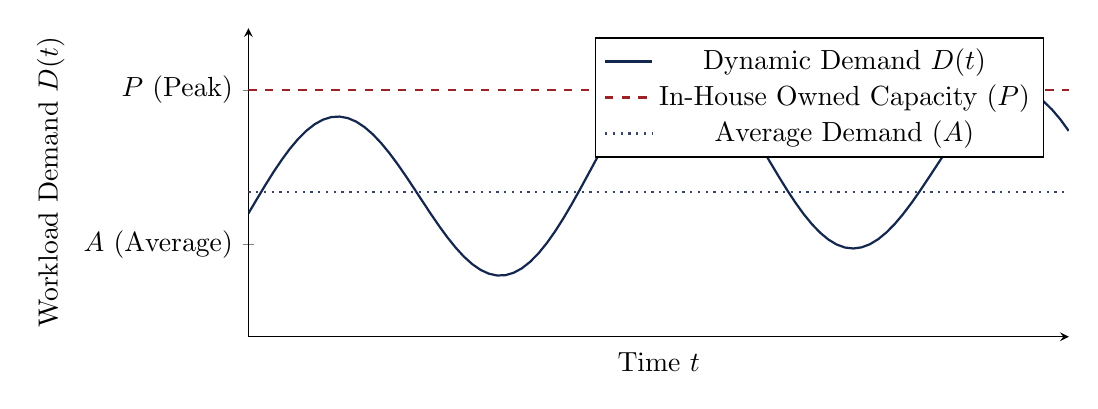
\begin{tikzpicture}
\begin{axis}[
    width=12cm, height=5.5cm,
    xlabel={Time $t$}, ylabel={Workload Demand $D(t)$},
    xmin=0, xmax=10, ymin=0, ymax=10,
    legend pos=north east,
    axis lines=left,
    xtick=\empty, ytick={3, 8},
    yticklabels={$A$ (Average), $P$ (Peak)}
]
\addplot[thick, navy, domain=0:10, samples=100] {5 + 3*sin(deg(x*1.5)) - cos(deg(x*0.5))};
\addlegendentry{Dynamic Demand $D(t)$}

\addplot[dashed, darkred, thick, domain=0:10] {8};
\addlegendentry{In-House Owned Capacity ($P$)}

\addplot[dotted, slate, thick, domain=0:10] {4.7};
\addlegendentry{Average Demand ($A$)}
\end{axis}
\end{tikzpicture}
\caption{Dynamic Demand vs In-House Static Over-Provisioning.}
\end{figure}

\subsection{Workload Penalty Integrals for Static Provisioning}
When an organization owns fixed resources $R(t)$, any divergence between available capacity $R(t)$ and instantaneous workload demand $D(t)$ incurs financial and operational penalties:
\begin{equation}
\text{Penalty Cost} \propto \int_{0}^{T} |D(t) - R(t)|\, dt
\end{equation}
\begin{itemize}[leftmargin=*]
  \item If $R(t) > D(t)$: The organization wastes capital paying for idle hardware, power, cooling, and software licensing.
  \item If $R(t) < D(t)$: The system suffers performance degradation, latency spikes, dropped transactions, and lost customer revenue.
\end{itemize}

Under exponential workload growth ($D(t) = e^t$), periodic static procurement with interval $t_p$ produces provisioning $R(t) = e^{t - t_p}$. The shortfall increases exponentially:
\begin{equation}
\text{Deficit}(t) = D(t) - R(t) = e^t - e^{t - t_p} = e^t (1 - e^{-t_p})
\end{equation}
demonstrating that fixed provisioning cycles can never keep pace with exponential demand growth.

\section{Big Data Architecture: Hadoop and HDFS}
\subsection{Hadoop Distributed File System (HDFS) Architecture}
HDFS is designed to store multi-terabyte and petabyte files reliably across large clusters of commodity hardware. It adopts a master/worker topology:
\begin{itemize}[leftmargin=*]
  \item \textbf{NameNode (Master):} Maintains the directory tree and file metadata in system RAM. File metadata maps filenames to a sequence of block IDs. Modifications are recorded durably in the \texttt{EditLog} on disk and consolidated periodically with the \texttt{FsImage} checkpoint file via the \textbf{Secondary NameNode}.
  \item \textbf{DataNodes (Workers):} Store actual data blocks as discrete files on local ext4/xfs filesystems. They handle block read/write operations from clients and emit heartbeat signals every 3 seconds to confirm node health.
\end{itemize}

\subsection{Block Size and Input Split Mathematics}
Unlike traditional filesystems with 4 KB disk clusters, HDFS employs very large block sizes (typically 64 MB, 128 MB, or 256 MB) to amortize disk seek times against sequential transfer rates.

When an input file of size $S$ is loaded into an HDFS cluster configured with block size $B$:
\begin{equation}
N_{\text{blocks}} = \left\lceil \frac{S}{B} \right\rceil
\end{equation}
In standard MapReduce configurations, Hadoop assigns exactly one \textbf{Mapper task} per logical \textbf{InputSplit} (which aligns 1:1 with HDFS physical blocks).

\begin{solved}{HDFS Mapper Task Allocation}
\Given An HDFS cluster operates with block size $B = 128\text{ MB}$. A client uploads an input file of size $S = 700\text{ MB}$ to execute a MapReduce job. Assuming default mapping of one map task per HDFS block, calculate the number of mapper tasks created.
\Formula
\begin{equation}
N_{\text{mappers}} = \left\lceil \frac{S}{B} \right\rceil
\end{equation}
\Steps
\begin{enumerate}[leftmargin=*]
  \item Decompose 700 MB across 128 MB block allocations:
  \begin{align*}
  \text{Block 1:} & \quad 128\text{ MB} & \text{Block 4:} & \quad 128\text{ MB}\\
  \text{Block 2:} & \quad 128\text{ MB} & \text{Block 5:} & \quad 128\text{ MB}\\
  \text{Block 3:} & \quad 128\text{ MB} & \text{Block 6:} & \quad 60\text{ MB} \quad (\text{Partial Block})
  \end{align*}
  \item Total allocated blocks: $5 \times 128\text{ MB} + 60\text{ MB} = 700\text{ MB} \implies 6\text{ blocks}$.
  \item Each block corresponds to an input split: $N_{\text{mappers}} = 6$.
\end{enumerate}
\Answer Exactly \textbf{6 mapper tasks} are spawned.
\end{solved}

\subsection{MapReduce Execution Pipeline: Partitioner vs Combiner}
The lecture highlights two critical intermediate optimization components in MapReduce:
\begin{itemize}[leftmargin=*]
  \item \textbf{Combiner (Mini-Reducer):} An \emph{optional} optimization component executed on the map worker node prior to network shuffle. It performs local pre-aggregation on intermediate key-value pairs (e.g., computing sub-totals in a word count job), drastically decreasing the volume of intermediate data transmitted across the cluster network. The execution of a Combiner is never guaranteed; Hadoop may run it zero, one, or multiple times depending on memory pressure.
  \item \textbf{Partitioner:} A \emph{mandatory} component that determines which physical Reducer instance receives each intermediate key. By default, Hadoop utilizes the \textbf{HashPartitioner}:
  \begin{equation}
  \text{Reducer ID} = (\text{key.hashCode()} \ \& \ \text{Integer.MAX\_VALUE}) \pmod{N_{\text{reducers}}}
  \end{equation}
  This guarantees that all intermediate values associated with the identical key arrive at the exact same Reducer node.
\end{itemize}

\section{Green Cloud Computing and Server Energy Dynamics}
\subsection{Data Center Energy Footprint and Efficiency Metrics}
Massive data centers consume hundreds of megawatts of electricity. Energy consumption is divided into two broad categories:
\begin{enumerate}[leftmargin=*]
  \item \textbf{IT Equipment Power ($P_{\text{IT}}$):} Compute servers, storage arrays, and network switches.
  \item \textbf{Infrastructure Overhead Power ($P_{\text{overhead}}$):} Chiller plants, cooling towers, fans, uninterruptible power supplies (UPS), power distribution units (PDUs), and facility lighting.
\end{enumerate}

\begin{defbox}{Power Usage Effectiveness (PUE) and DCiE}
The industry standard metric established by The Green Grid is \textbf{Power Usage Effectiveness (PUE)}:
\begin{equation}
\text{PUE} = \frac{\text{Total Facility Power}}{\text{IT Equipment Power}} = \frac{P_{\text{IT}} + P_{\text{overhead}}}{P_{\text{IT}}} \ge 1.0
\end{equation}
A PUE of $2.0$ indicates that for every 1 Watt powering servers, another 1 Watt is consumed by cooling and power delivery. Modern hyperscale facilities (Google, Microsoft) achieve PUE values between $1.1$ and $1.2$.\\
The inverse metric is \textbf{Data Center Infrastructure Efficiency (DCiE)}:
\begin{equation}
\text{DCiE} = \frac{1}{\text{PUE}} \times 100\%
\end{equation}
\end{defbox}

\subsection{Server Power Dynamics and Core Utilization}
A physical server's power consumption is not static; it scales with CPU utilization and active hardware components:
\begin{equation}
P(u) = P_{\text{idle}} + (P_{\text{peak}} - P_{\text{idle}}) \times u
\end{equation}
where $P_{\text{idle}}$ is the idle power draw (typically $50\%$ to $60\%$ of peak power $P_{\text{peak}}$), and $u \in [0, 1]$ represents CPU utilization.

\begin{thmbox}{Impact of Dynamic Core Activation on Power Draw}
When a multi-core server detects a workload spike and dynamically switches CPU cores from low-power C-states (sleep states) to active C0 execution states:
\begin{enumerate}[leftmargin=*]
  \item Each active core draws dynamic switching power: $P_{\text{dynamic}} = \alpha \cdot C_L \cdot V^2 \cdot f$ (where $\alpha$ is activity factor, $C_L$ load capacitance, $V$ operating voltage, and $f$ clock frequency).
  \item Static leakage current power increases proportionally with core temperature.
  \item \textbf{Net Effect:} Total server power consumption \textbf{increases} as additional CPU cores become active, even if workload execution time per core drops.
\end{enumerate}
\end{thmbox}

\section{Comprehensive Solved Assignment Problems (Week 5)}

\begin{solved}{SLA Downtime Allowance Calculation}
\Given A cloud provider commits to a 99\% uptime SLA. The client's application runs 12 hours/day for 30 days. Find maximum allowable downtime.
\Steps
\begin{equation}
T_{\text{scheduled}} = 12\text{ h/day} \times 30\text{ days} = 360\text{ hours}
\end{equation}
\begin{equation}
T_{\text{allowed downtime}} = (1 - 0.99) \times 360 = 0.01 \times 360 = 3.6\text{ hours}
\end{equation}
\Answer \textbf{3.6 hours}.
\end{solved}

\begin{solved}{Multi-Core Server Power Consumption}
\Given A cloud server dynamically activates additional CPU cores to handle a sudden surge in user requests.
\Steps
\begin{enumerate}[leftmargin=*]
  \item Activating dormant processor cores draws additional dynamic switching power and leakage current.
  \item While techniques like DVFS reduce voltage at lower frequencies, adding active cores increases total aggregate wattage drawn by the system.
\end{enumerate}
\Answer \textbf{Power consumption increases as additional CPU cores become active}.
\end{solved}

\begin{solved}{Mitigating Upfront Capital Expenditure}
\Given Which cloud characteristic directly eliminates massive upfront hardware purchases?
\Steps
\begin{enumerate}[leftmargin=*]
  \item \textbf{Pay-as-you-go pricing} converts Capital Expenditure (CapEx) into Operational Expenditure (OpEx), allowing organizations to pay strictly for consumed compute time and storage without purchasing servers upfront.
\end{enumerate}
\Answer \textbf{Pay-as-you-go pricing}.
\end{solved}

\begin{solved}{HDFS Block Input Splits and Map Tasks}
\Given Block size $B = 128\text{ MB}$, input file $S = 700\text{ MB}$.
\Steps
\begin{equation}
N = \left\lceil \frac{700}{128} \right\rceil = \left\lceil 5.46875 \right\rceil = 6
\end{equation}
\Answer \textbf{6}.
\end{solved}

\begin{solved}{Primary Virtualization Management Entity}
\Given Identify the virtualization layer component responsible for creating, running, and managing virtual machines.
\Steps
\begin{enumerate}[leftmargin=*]
  \item The \textbf{Hypervisor} (or Virtual Machine Monitor, VMM) abstracts physical hardware resources and mediates guest virtual machine execution.
\end{enumerate}
\Answer \textbf{Hypervisor}.
\end{solved}

\begin{solved}{MapReduce Key-to-Reducer Assignment}
\Given Identify the MapReduce subsystem that routes each intermediate key to its designated Reducer.
\Steps
\begin{enumerate}[leftmargin=*]
  \item The \textbf{Partitioner} calculates the destination reducer index for each key (typically via hash modulo operations).
\end{enumerate}
\Answer \textbf{Partitioner}.
\end{solved}

\begin{solved}{Optional MapReduce Optimization Phase}
\Given Identify the MapReduce component that is optional and may execute zero, one, or multiple times.
\Steps
\begin{enumerate}[leftmargin=*]
  \item The \textbf{Combiner} operates as a semi-reducer on local map output. Hadoop does not guarantee its execution; therefore, MapReduce job logic must remain algebraically valid even when the Combiner is skipped entirely.
\end{enumerate}
\Answer \textbf{Combiner}.
\end{solved}

\begin{solved}{Data Center Energy Consumption Contributors}
\Given Which data center subsystems contribute directly to overall energy consumption?
\Steps
\begin{enumerate}[leftmargin=*]
  \item IT server equipment (processors, memory, disks).
  \item Air conditioning chillers, cooling towers, and ventilation fans.
  \item Power distribution units (PDUs) and uninterruptible power supply (UPS) transformers.
\end{enumerate}
\Answer \textbf{All of the above}.
\end{solved}

\begin{solved}{Server Consolidation Impact on Green Computing}
\Given How does server consolidation via live VM migration promote green cloud computing?
\Steps
\begin{enumerate}[leftmargin=*]
  \item Packing virtual machines onto fewer physical hosts allows underutilized hosts to be powered down into deep sleep states, eliminating idle power waste.
\end{enumerate}
\Answer \textbf{Reduces total energy consumption by powering down idle physical servers}.
\end{solved}

\begin{solved}{HDFS Data Integrity and Fault Tolerance}
\Given How does HDFS achieve fault tolerance against DataNode drive crashes without relying on RAID hardware?
\Steps
\begin{enumerate}[leftmargin=*]
  \item HDFS replicates each data block across multiple physically independent DataNodes (default replication factor $R = 3$) with rack awareness.
\end{enumerate}
\Answer \textbf{Block Replication across multiple nodes}.
\end{solved}

% ==================================================================
%  WEEK 6
% ==================================================================
\chapter{Cloud Security, Privacy, and Trust Management}

\section{Introduction and Week Overview}
Week 6 establishes the theoretical and operational foundations of security in multi-tenant cloud environments. The curriculum systematically progresses through four integrated modules:
\begin{enumerate}[leftmargin=*]
  \item \textbf{Foundational Security Primitives and the CIA Triad:} Mathematical definitions of Confidentiality, Integrity, and Availability; formal models of security policy versus enforcement mechanisms.
  \item \textbf{Attack Taxonomy and Attack Lifecycles:} The four classical structural attacks (Interruption, Interception, Modification, Fabrication); Passive vs Active attacks; reconnaissance, scanning, and exploitation phases.
  \item \textbf{Identity, Authentication, and Authorization:} Deep distinction between Authentication (AuthN) and Authorization (AuthZ); federated protocols (SAML 2.0 and OAuth 2.0); Role-Based Access Control (RBAC).
  \item \textbf{Virtualization Vulnerabilities and Gartner Cloud Risks:} Cross-VM side-channel attacks, cache timing analysis, hypervisor escape, and Gartner's seven cardinal cloud security risks.
\end{enumerate}

\section{Foundational Security Primitives: The CIA Triad}
Security in distributed systems rests upon three core pillars known as the \textbf{CIA Triad}:
\begin{figure}[H]
\centering
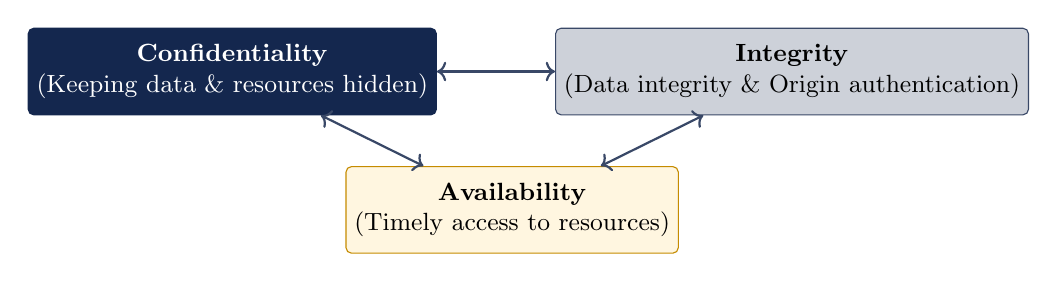
\begin{tikzpicture}[node distance=1.8cm, font=\small]
  \node[dark, minimum width=3.8cm, minimum height=1.1cm] (c) {\textbf{Confidentiality}\\(Keeping data \& resources hidden)};
  \node[mid, right=1.5cm of c, minimum width=3.8cm, minimum height=1.1cm] (i) {\textbf{Integrity}\\(Data integrity \& Origin authentication)};
  \node[gold, below=1.2cm of $(c)!0.5!(i)$, minimum width=4.2cm, minimum height=1.1cm] (a) {\textbf{Availability}\\(Timely access to resources)};

  \draw[arr, <->] (c) -- (i);
  \draw[arr, <->] (i) -- (a);
  \draw[arr, <->] (a) -- (c);
\end{tikzpicture}
\caption{The Classical CIA Triad in Cloud Computing.}
\end{figure}

\begin{itemize}[leftmargin=*]
  \item \textbf{Confidentiality:} Preventing the unauthorized disclosure of sensitive information. Cryptographic controls (such as AES-256 for data at rest and TLS 1.3 for data in transit) ensure confidentiality.
  \item \textbf{Integrity:} Guaranteeing that data has not been altered, modified, corrupted, or deleted by unauthorized parties or malfunctioning software. It encompasses:
    \begin{itemize}
      \item \emph{Data Integrity:} State verification ensuring data matches its original format (enforced via SHA-256 cryptographic hashes and HMACs).
      \item \emph{Origin Integrity (Authenticity):} Guaranteeing the genuine origin of the data or service identity.
    \end{itemize}
  \item \textbf{Availability:} Ensuring authorized users have uninterrupted, timely access to computing resources, data stores, and network endpoints without unexpected denial of service.
\end{itemize}

\begin{warnbox}{Integrity Failure Despite Perfect Encryption}
A common misconception is that encryption automatically guarantees data integrity. Encryption scrambles data to preserve \textbf{Confidentiality}. If an administrator or erroneous application software bug alters database entries (e.g., corrupting financial ledger balances), the data remains confidential (still encrypted) but its \textbf{Integrity} is completely destroyed!
\end{warnbox}

\section{Structural Attack Taxonomy}
Prof. Ghosh classifies security violations into four canonical architectural attack patterns based on the source ($S$), destination ($D$), and interceptor ($I$):

\begin{center}
\begin{tabularx}{\textwidth}{>{\bfseries}l l p{3.2cm} X}
\toprule
Attack Type & Violated Property & Structural Mechanism & Concrete Real-World Example\\
\midrule
Interruption & Availability & Attacker destroys or severs the communication path between $S$ and $D$. & Distributed Denial of Service (DDoS), physical fiber cut, RAM starvation.\\
Interception & Confidentiality & Attacker secretly monitors or taps the link, reading packets without altering them. & Packet sniffing via Wireshark, optical fiber tapping, eavesdropping.\\
Modification & Integrity & Attacker intercepts legitimate packets from $S$, alters payload bits, and forwards them to $D$. & Man-in-the-Middle (MitM) payload alteration, SQL injection data corruption.\\
Fabrication & Authenticity & Attacker injects spurious, counterfeit messages into the system claiming to originate from $S$. & DNS spoofing, phishing portals, fake VPN login gateways, ARP poisoning.\\
\bottomrule
\end{tabularx}
\end{center}

\begin{figure}[H]
\centering
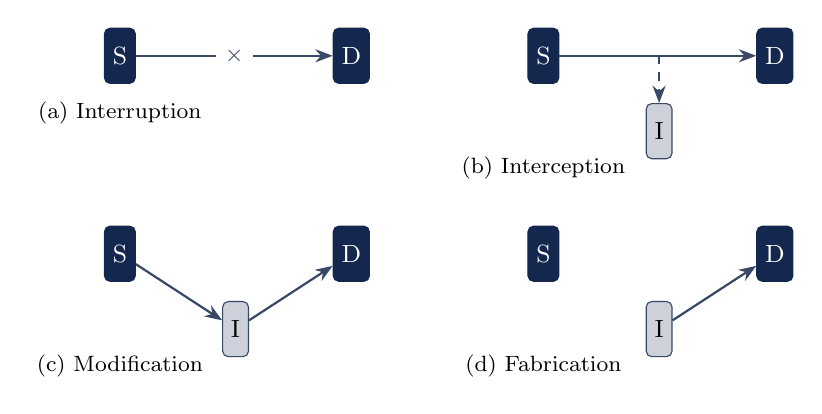
\begin{tikzpicture}[node distance=1.5cm, font=\footnotesize]
  % Interruption
  \node[dark] (s1) {S}; \node[dark, right=2.5cm of s1] (d1) {D};
  \draw[arr] (s1) -- node[midway, fill=white] {$\times$} (d1);
  \node[below=0.1cm of s1] {(a) Interruption};

  % Interception
  \node[dark, right=2cm of d1] (s2) {S}; \node[dark, right=2.5cm of s2] (d2) {D};
  \node[mid, below=0.6cm of $(s2)!0.5!(d2)$] (i2) {I};
  \draw[arr] (s2) -- (d2); \draw[arr, dashed] ($(s2)!0.5!(d2)$) -- (i2);
  \node[below=0.8cm of s2] {(b) Interception};

  % Modification
  \node[dark, below=1.8cm of s1] (s3) {S}; \node[dark, right=2.5cm of s3] (d3) {D};
  \node[mid, below=0.6cm of $(s3)!0.5!(d3)$] (i3) {I};
  \draw[arr] (s3) -- (i3); \draw[arr] (i3) -- (d3);
  \node[below=0.8cm of s3] {(c) Modification};

  % Fabrication
  \node[dark, right=2cm of d3] (s4) {S}; \node[dark, right=2.5cm of s4] (d4) {D};
  \node[mid, below=0.6cm of $(s4)!0.5!(d4)$] (i4) {I};
  \draw[arr] (i4) -- (d4);
  \node[below=0.8cm of s4] {(d) Fabrication};
\end{tikzpicture}
\caption{Four Fundamental Classes of Structural Security Attacks.}
\end{figure}

\subsection{Passive vs Active Attacks}
\begin{itemize}[leftmargin=*]
  \item \textbf{Passive Attacks:} The attacker monitors, inspects, or analyzes network transmissions without injecting, modifying, or delaying data packets.
    \begin{itemize}
      \item Examples: Eavesdropping, network packet sniffing, traffic volume/timing analysis.
      \item Operational Implication: Extremely difficult to detect because the system continues functioning normally. Primary defense is proactive \textbf{prevention} via strong end-to-end encryption.
    \end{itemize}
  \item \textbf{Active Attacks:} The attacker actively alters the data stream, creates false streams, disrupts server operation, or modifies system states.
    \begin{itemize}
      \item Examples: Session hijacking, replay attacks, man-in-the-middle tampering, masquerading, Denial of Service (DoS).
      \item Operational Implication: Can be detected via integrity checks, sequence numbers, and anomaly monitoring; focus is on \textbf{detection and rapid automated recovery}.
    \end{itemize}
\end{itemize}

\subsection{The Multi-Phase Attack Lifecycle}
A sophisticated adversary typically executes attacks in structured operational phases:
\begin{enumerate}[leftmargin=*]
  \item \textbf{Reconnaissance (Information Gathering):} Collecting target intelligence without actively exploiting systems.
    \begin{itemize}
      \item \emph{Passive Reconnaissance:} Scraping public databases, social media, WHOIS records, and DNS records.
      \item \emph{Active Reconnaissance:} DNS zone transfers, ping sweeps, and network service mapping.
    \end{itemize}
  \item \textbf{Scanning and Probing:} Using port scanners (e.g., Nmap) and vulnerability scanners to discover listening network services, operating system versions, and known unpatched CVE vulnerabilities.
  \item \textbf{Gaining Access (Exploitation):} Executing targeted exploit payloads (such as buffer overflow attacks, SQL injections, or remote code execution) to bypass security boundaries and achieve administrative privileges.
  \item \textbf{Maintaining Access and Persistence:} Installing stealth rootkits, trojans, or backdoor SSH keys to retain control across server reboots.
  \item \textbf{Covering Tracks:} Altering or deleting system log files (\texttt{/var/log/auth.log}), resetting file modification timestamps, and disabling intrusion detection alerts.
\end{enumerate}

\section{Identity Management: Authentication vs Authorization}
A central security theme emphasized in Week 6 is the crisp formal distinction between Authentication and Authorization:

\begin{center}
\begin{tabularx}{\textwidth}{>{\bfseries}l p{6.5cm} X}
\toprule
Dimension & Authentication (AuthN) & Authorization (AuthZ)\\
\midrule
Core Question & ``Who are you?'' (Verification of Identity) & ``What actions are you permitted to execute?''\\
Mechanism & Verification of digital credentials (passwords, cryptographic tokens, biometric signatures, MFA). & Evaluation of permissions, Access Control Lists (ACLs), or Role-Based policies (RBAC).\\
Timing & Occurs \textbf{first} at system ingress before session establishment. & Evaluated \textbf{continuously} whenever an authenticated subject attempts an operation.\\
Protocol Standards & Kerberos, OpenID Connect (OIDC), SAML 2.0 Identity Assertion, FIDO2 / WebAuthn. & OAuth 2.0 (access tokens and scopes), XACML, AWS IAM Policy documents.\\
Failure Result & HTTP 401 Unauthorized (Unauthenticated identity). & HTTP 403 Forbidden (Identity verified, but lacks sufficient permissions).\\
\bottomrule
\end{tabularx}
\end{center}

\begin{defbox}{Security Assertion Markup Language (SAML 2.0) vs OAuth 2.0}
\textbf{SAML 2.0:} An XML-based federated protocol designed primarily for cross-domain Web Single Sign-On (\textbf{Authentication}). An Identity Provider (IdP) signs an XML assertion containing identity attributes and transmits it to a Service Provider (SP) via the user's browser.\\
\textbf{OAuth 2.0:} A lightweight, JSON-based framework designed for delegated \textbf{Authorization}. It issues short-lived Access Tokens (such as JSON Web Tokens, JWTs) granting a third-party client scoped access to a user's protected resources on a Resource Server without revealing user credentials.
\end{defbox}

\section{Virtualization Security and Multi-Tenancy Exploits}
\subsection{Hypervisor Isolation and Virtual Machine Escape}
In a public cloud, multiple untrusted virtual machines co-exist on the same physical bare-metal host. The hypervisor (Virtual Machine Monitor, VMM) is responsible for enforcing strict isolation:
\begin{itemize}[leftmargin=*]
  \item \textbf{VM Escape:} The most catastrophic virtualization exploit, where code running inside a guest operating system breaks out of the virtualized sandbox and interacts directly with the host hypervisor or host OS kernel. Once escaped, the attacker acquires total control over all co-located tenant VMs on that physical server.
\end{itemize}

\subsection{Cross-VM Side-Channel Attacks (Ristenpart et al.)}
In their seminal 2009 research paper (\emph{Hey, You, Get Off of My Cloud: Exploring Information Leakage in Third-Party Compute Clouds}), Ristenpart et al. demonstrated that physical resource sharing in public clouds (specifically Amazon EC2) introduces subtle side-channel vulnerabilities:

\begin{enumerate}[leftmargin=*]
  \item \textbf{Co-Residence Verification:} An attacker probes cloud IP ranges to identify the target victim's network address. By exploiting internal network topologies (comparing Dom0 IP hops and round-trip ping times $\le 1\text{ ms}$), the attacker verifies that their own VM resides on the identical physical hardware as the victim.
  \item \textbf{Shared Hardware Contention:} Even when CPU registers and memory pages are strictly isolated by hardware MMU page tables, physical cores share hardware caches:
    \begin{itemize}
      \item L1 / L2 caches (per core) and unified \textbf{L3 Last Level Cache (LLC)}.
      \item Memory buses, CPU branch target buffers (BTB), and hyperthreading pipelines.
    \end{itemize}
  \item \textbf{Cache-Timing Side Channels (Prime + Probe):}
    \begin{itemize}
      \item \emph{Prime Phase:} The attacker fills specific cache sets with their own data lines.
      \item \emph{Idle Window:} The attacker waits while the victim VM executes cryptographic operations (such as modular exponentiation during RSA signing).
      \item \emph{Probe Phase:} The attacker re-reads their own cached memory addresses, timing the access latency. Memory addresses that were evicted by the victim take longer to reload from main RAM.
      \item \emph{Key Extraction:} By observing which cache sets experienced evictions, the attacker reconstructs internal CPU access patterns, leaking private cryptographic keys without ever violating memory permissions!
    \end{itemize}
\end{enumerate}

\section{Gartner's Seven Cardinal Cloud Security Risks}
The lecture highlights the influential risk taxonomy published by Gartner for enterprise cloud computing adopters:
\begin{enumerate}[leftmargin=*]
  \item \textbf{Privileged User Access:} Cloud providers maintain system administrators with root access to physical hosts and virtualization hypervisors. Organizations must demand strict administrative auditing, background vetting, and cryptographic envelope encryption.
  \item \textbf{Regulatory Compliance:} Enterprises remain legally liable for data compliance (HIPAA, PCI-DSS, ISO 27001) even when data is hosted externally. Providers must submit to external third-party compliance audits.
  \item \textbf{Data Location and Sovereignty:} Cloud consumers often cannot specify the exact physical storage medium or geographic jurisdiction where data is stored. Trans-border data movement may violate national data residency laws (e.g., GDPR in the European Union or local data sovereignty mandates).
  \item \textbf{Data Segregation / Isolation:} In shared multi-tenant databases and SAN volumes, data from competing corporations resides on adjacent disk sectors. Multi-tenant encryption schemes must guarantee complete logical segregation.
  \item \textbf{Recovery and Business Continuity:} In the event of catastrophic physical outages or ransomware events at the provider's facility, providers must have verified Recovery Point Objectives (RPO) and Recovery Time Objectives (RTO).
  \item \textbf{Investigative Support (E-Discovery):} Conducting forensic investigations or digital discovery in a multi-tenant cloud is exceptionally difficult without violating the privacy rights of other co-located tenants.
  \item \textbf{Long-Term Viability:} What happens to an organization's mission-critical data if the cloud provider goes bankrupt, gets acquired by a hostile competitor, or abruptly terminates service? Data portability and non-proprietary exit strategies are essential.
\end{enumerate}

\section{Comprehensive Solved Assignment Problems (Week 6)}

\begin{solved}{Database Bug and Security Objective Failure}
\Given A database stores encrypted customer records. An administrator erroneously alters account balances due to an unhandled application bug. Identify the security objective that failed.
\Steps
\begin{enumerate}[leftmargin=*]
  \item Encryption preserves \textbf{Confidentiality} (unauthorized parties cannot read the records).
  \item Availability is intact because users can still query the system.
  \item Erroneous or unauthorized modification of data directly compromises \textbf{Integrity}.
\end{enumerate}
\Answer \textbf{Integrity only}.
\end{solved}

\begin{solved}{Fake VPN Portal Exploitation}
\Given An employee visits a fake VPN portal that visually imitates the legitimate corporate login page. Before any credentials are typed, which security property has failed?
\Steps
\begin{enumerate}[leftmargin=*]
  \item No confidential password has been disclosed yet.
  \item The fraudulent portal is masquerading as the genuine corporate gateway (a fabrication attack).
  \item The security property that is broken is \textbf{Authenticity} (the claim of genuine identity).
\end{enumerate}
\Answer \textbf{Authenticity}.
\end{solved}

\begin{solved}{Classification of Active vs Passive Attacks}
\Given Identify which attack is NOT considered a passive attack among: Packet sniffing, Traffic analysis, Session hijacking, Network monitoring.
\Steps
\begin{enumerate}[leftmargin=*]
  \item Packet sniffing, traffic analysis, and network monitoring merely inspect transmission without altering packets (Passive).
  \item \textbf{Session hijacking} actively injects malicious packets, alters sequence numbers, or terminates the user's connection to seize control of the session (Active).
\end{enumerate}
\Answer \textbf{Session hijacking}.
\end{solved}

\begin{solved}{Inability to Modify Transmitted Payloads}
\Given Which attack cannot directly modify the contents of transmitted data?
\Steps
\begin{enumerate}[leftmargin=*]
  \item Replay attacks inject recorded packets; MitM attacks alter bits in flight; Masquerading sends forged data.
  \item \textbf{Eavesdropping} is purely passive listening and cannot modify data contents.
\end{enumerate}
\Answer \textbf{Eavesdropping}.
\end{solved}

\begin{solved}{Denial of Service (DoS) Characteristics}
\Given What best describes a Denial-of-Service attack?
\Steps
\begin{enumerate}[leftmargin=*]
  \item An adversary floods servers or networks with overwhelming request volumes, consuming compute/bandwidth resources so legitimate users cannot access the service.
\end{enumerate}
\Answer \textbf{An attacker floods a server with excessive requests, making the service unavailable to legitimate users}.
\end{solved}

\begin{solved}{Reconnaissance vs Exploitation Phase}
\Given Identify the activity least likely to be considered part of the reconnaissance phase.
\Steps
\begin{enumerate}[leftmargin=*]
  \item DNS enumeration, port scanning, and searching public websites are reconnaissance activities.
  \item \textbf{Exploiting a buffer overflow} to gain root access is part of the active \emph{Exploitation} phase, not reconnaissance.
\end{enumerate}
\Answer \textbf{Exploiting a buffer overflow vulnerability to gain administrator privileges}.
\end{solved}

\begin{solved}{Authentication vs Authorization Statements}
\Given Evaluate:
\begin{itemize}
  \item Statement I: Authentication determines whether a user is allowed to access a resource.
  \item Statement II: Authorization determines what actions an authenticated user is permitted to perform.
\end{itemize}
\Steps
\begin{enumerate}[leftmargin=*]
  \item Statement I is FALSE: Authentication verifies \emph{identity} (who the user is), not whether they are allowed to access a specific resource.
  \item Statement II is TRUE: Authorization evaluates permissions to determine permitted actions.
\end{enumerate}
\Answer \textbf{Statement I is False, and Statement II is True}.
\end{solved}

\begin{solved}{Data Location and Sovereignty Concerns}
\Given A multinational corporation stores EU citizen records in a US-based cloud data center and faces legal scrutiny under GDPR. Which Gartner cloud risk applies?
\Steps
\begin{enumerate}[leftmargin=*]
  \item European privacy mandates require personal citizen data to reside within compliant jurisdictions.
  \item Moving data across geographic borders directly triggers \textbf{Data Location and Sovereignty} risk.
\end{enumerate}
\Answer \textbf{Data Location}.
\end{solved}

\begin{solved}{Multi-Tenant Cache-Timing Exploits}
\Given How does an attacker extract private cryptographic keys in a cross-VM side-channel attack?
\Steps
\begin{enumerate}[leftmargin=*]
  \item By establishing co-residence on the same physical CPU socket and monitoring access latencies to shared L3 CPU cache lines (Prime+Probe technique).
\end{enumerate}
\Answer \textbf{By measuring CPU cache access latency on shared physical hardware}.
\end{solved}

\begin{solved}{Hypervisor Sandbox Escape Threat}
\Given What is the security impact of a successful VM Escape vulnerability?
\Steps
\begin{enumerate}[leftmargin=*]
  \item The attacker breaks through guest OS virtualization barriers to execute arbitrary code with host hypervisor privileges, compromising all co-located tenant VMs.
\end{enumerate}
\Answer \textbf{The attacker gains direct access to the host hypervisor, compromising all tenant VMs on the physical host}.
\end{solved}

% ==================================================================
%  WEEK 7
% ==================================================================
\chapter{Mobile Cloud Computing, Cloudlets, and Geospatial Cloud}

\section{Introduction and Week Overview}
Week 7 explores the convergence of cloud computing with mobile handheld devices and geographic information systems. The curriculum addresses computational scarcity at the network edge through three fundamental themes:
\begin{enumerate}[leftmargin=*]
  \item \textbf{Mobile Cloud Computing (MCC):} Architectural models augmenting battery-constrained, CPU-limited mobile devices with remote cloud resources; runtime partitioning and computation offloading.
  \item \textbf{Mathematical Formulation of Energy-Aware Offloading:} Derivation of the Kumar and Lu energy saving conditions, transmission delays, idle listening power, and numerical break-even analysis.
  \item \textbf{Cloudlets and Low-Latency Edge Computing:} Three-tier hierarchical architecture (Mobile $\to$ Cloudlet $\to$ Distant Cloud), transient virtual machine synthesis, and real-time augmented reality constraints.
  \item \textbf{Geospatial Cloud Computing:} Spatial Data Infrastructure (SDI), Open Geospatial Consortium (OGC) web services, massive spatial data storage, and distributed spatial indexing.
\end{enumerate}

\section{Mobile Cloud Computing (MCC) Foundations}
\subsection{Motivation and Intrinsic Hardware Constraints}
Despite dramatic improvements in mobile hardware, smartphones and IoT edge devices remain fundamentally constrained compared to server infrastructure:
\begin{itemize}[leftmargin=*]
  \item \textbf{Battery Energy Capacity:} Electrochemical battery energy density grows at less than $5\%$ to $8\%$ annually, whereas mobile application computational demands (computer vision, speech synthesis, 3D gaming) grow exponentially.
  \item \textbf{Thermal Dissipation Limits:} Passive cooling restricts sustained high-frequency CPU/GPU execution to avoid thermal throttling.
  \item \textbf{Network Variability:} Wireless connections (4G/5G, Wi-Fi) suffer from variable bandwidth, signal fading, packet loss, and handoff delays.
\end{itemize}

\begin{defbox}{Mobile Cloud Computing (MCC)}
\textbf{Mobile Cloud Computing (MCC)} integrates cloud computing into mobile environments to overcome hardware limitations. Computation-intensive and data-heavy tasks are dynamically extracted from the mobile device and processed on remote cloud infrastructure, delivering results back across wireless networks.
\end{defbox}

\begin{figure}[H]
\centering
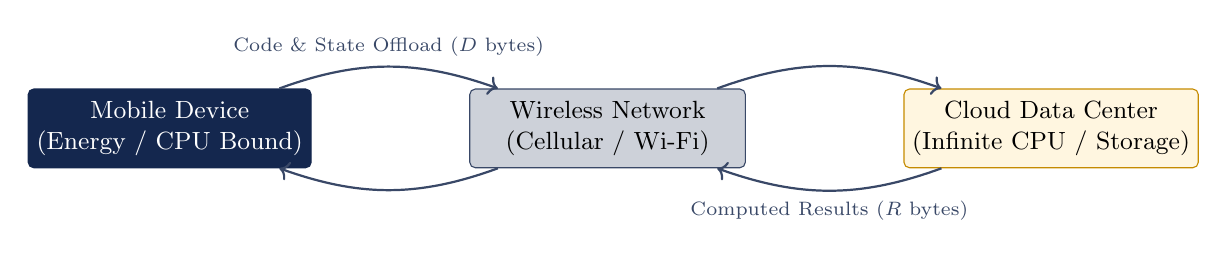
\begin{tikzpicture}[node distance=1.2cm, font=\small]
  \node[dark, minimum width=3cm, minimum height=1cm] (mob) {Mobile Device\\(Energy / CPU Bound)};
  \node[mid, right=2cm of mob, minimum width=3.5cm, minimum height=1cm] (net) {Wireless Network\\(Cellular / Wi-Fi)};
  \node[gold, right=2cm of net, minimum width=3.5cm, minimum height=1cm] (cloud) {Cloud Data Center\\(Infinite CPU / Storage)};

  \draw[arr, ->] (mob) to[bend left=20] node[above, font=\scriptsize] {Code \& State Offload ($D$ bytes)} (net);
  \draw[arr, ->] (net) to[bend left=20] (cloud);
  \draw[arr, ->] (cloud) to[bend left=20] node[below, font=\scriptsize] {Computed Results ($R$ bytes)} (net);
  \draw[arr, ->] (net) to[bend left=20] (mob);
\end{tikzpicture}
\caption{Classical Mobile Cloud Computation Offloading Architecture.}
\end{figure}

\subsection{Workload Suitability for Offloading}
Not all mobile computational tasks are candidates for cloud offloading:
\begin{itemize}[leftmargin=*]
  \item \textbf{Highly Suitable Tasks:} High computational complexity paired with small data exchange (High Compute-to-Data Ratio).
    \begin{itemize}
      \item Complex mathematical simulations, video encoding/transcoding, optical character recognition (OCR), deep learning inference, natural language processing.
    \end{itemize}
  \item \textbf{Unsuitable Tasks:}
    \begin{itemize}
      \item \emph{Hard Real-Time Tasks:} Tasks requiring deterministic sub-millisecond response times (e.g., autonomous vehicle collision avoidance, sensor stabilization). Network latency jitter makes remote cloud offloading hazardous.
      \item \emph{Data-Heavy Tasks with Minimal Compute:} Tasks where wireless data transmission energy exceeds local computation energy (e.g., streaming uncompressed sensor readings without local processing).
      \item \emph{Hardware-Coupled Tasks:} Code requiring direct physical hardware access (accelerometer reads, camera frame grabbing, display rendering).
    \end{itemize}
\end{itemize}

\section{Mathematical Formulation of Computation Offloading}
\subsection{System Model and Parameters}
Following the formal analytical model established by Kumar and Lu (IEEE Computer):
\begin{itemize}[leftmargin=*]
  \item $C$: Total computational complexity of the workload (number of CPU instructions).
  \item $M$: Execution speed of the mobile device processor (instructions per second).
  \item $F$: Cloud acceleration factor ($F \gg 1$), such that the cloud executes at speed $F \cdot M$ instructions per second.
  \item $D$: Volume of application data and program state transferred over the wireless uplink (bytes).
  \item $B$: Usable wireless transmission bandwidth (bytes per second).
  \item $P_c$: Power consumed by the mobile device CPU during active local computation (Watts).
  \item $P_{\text{tr}}$: Power consumed by the mobile wireless transceiver during active transmission (Watts).
  \item $P_i$: Power consumed by the mobile device in the idle state while awaiting cloud responses (Watts).
\end{itemize}

\subsection{Energy Consumption Derivations}
\subsubsection{Local Execution Energy ($E_{\text{local}}$)}
The time required to compute the workload locally on the mobile device is:
\begin{equation}
t_{\text{local}} = \frac{C}{M}
\end{equation}
The total electrical energy consumed by local processing is:
\begin{equation}
E_{\text{local}} = P_c \times t_{\text{local}} = P_c \left( \frac{C}{M} \right)
\end{equation}

\subsubsection{Cloud Offloading Energy ($E_{\text{cloud}}$)}
When offloading, the mobile device incurs energy in two sequential stages:
\begin{enumerate}[leftmargin=*]
  \item \textbf{Transmission Stage:} Transmitting $D$ bytes across the network at bandwidth $B$:
  \begin{equation}
  t_{\text{tx}} = \frac{D}{B}, \quad E_{\text{tx}} = P_{\text{tr}} \times t_{\text{tx}} = P_{\text{tr}} \left( \frac{D}{B} \right)
  \end{equation}
  \item \textbf{Idle Wait Stage:} Awaiting computation completion while the cloud processes the workload at speed $F \cdot M$:
  \begin{equation}
  t_{\text{cloud}} = \frac{C}{F \cdot M}, \quad E_{\text{idle}} = P_i \times t_{\text{cloud}} = P_i \left( \frac{C}{F \cdot M} \right)
  \end{equation}
\end{enumerate}
Summing the transmission and idle listening energies (assuming negligible result return payload):
\begin{equation}
E_{\text{cloud}} = E_{\text{tx}} + E_{\text{idle}} = P_{\text{tr}} \left( \frac{D}{B} \right) + P_i \left( \frac{C}{F \cdot M} \right)
\end{equation}

\begin{thmbox}{Energy Conservation Offloading Threshold Theorem}
Offloading saves energy if and only if $E_{\text{cloud}} < E_{\text{local}}$, yielding net savings $\Delta E > 0$:
\begin{equation}
\Delta E = E_{\text{local}} - E_{\text{cloud}} = P_c \left( \frac{C}{M} \right) - \left[ P_{\text{tr}} \left( \frac{D}{B} \right) + P_i \left( \frac{C}{F \cdot M} \right) \right] > 0
\end{equation}
Rearranging to isolate the transmission time $t_{\text{tx}} = \frac{D}{B}$:
\begin{equation}
P_{\text{tr}} \left( \frac{D}{B} \right) < \frac{C}{M} \left( P_c - \frac{P_i}{F} \right)
\end{equation}
\begin{equation}
\frac{D}{B} < \frac{C}{M} \left( \frac{P_c - P_i / F}{P_{\text{tr}}} \right)
\end{equation}
\textbf{Physical Meaning:} Offloading is energy-efficient if the time to transmit the input data ($D/B$) is strictly less than the local compute duration ($C/M$) scaled by the relative power differential ratio $\frac{P_c - P_i/F}{P_{\text{tr}}}$.
\end{thmbox}

\begin{solved}{Offloading Energy Savings Calculation (Lecture Numerical Example)}
\Given A mobile device executes a computer vision task with parameters:
\begin{itemize}
  \item Workload complexity: $C = 1.2 \times 10^9\text{ instructions}$.
  \item Mobile compute speed: $M = 6 \times 10^8\text{ inst/s}$ ($600\text{ MIPS}$).
  \item Cloud speedup multiplier: $F = 10$ ($F \cdot M = 6 \times 10^9\text{ inst/s}$).
  \item Data to transmit: $D = 3\text{ MB}$.
  \item Network throughput: $B = 2\text{ MB/s}$.
  \item Power coefficients: $P_c = 1.8\text{ W}$, $P_{\text{tr}} = 1.4\text{ W}$, $P_i = 0.2\text{ W}$.
\end{itemize}
\Formula
\begin{equation}
\Delta E = P_c \left(\frac{C}{M}\right) - P_{\text{tr}} \left(\frac{D}{B}\right) - P_i \left(\frac{C}{F \cdot M}\right)
\end{equation}
\Steps
\begin{enumerate}[leftmargin=*]
  \item \textbf{Local Execution Evaluation:}
  \begin{equation}
  t_{\text{local}} = \frac{1.2 \times 10^9}{6 \times 10^8} = 2.0\text{ seconds}
  \end{equation}
  \begin{equation}
  E_{\text{local}} = 1.8\text{ W} \times 2.0\text{ s} = 3.60\text{ Joules}
  \end{equation}
  \item \textbf{Cloud Offloading Evaluation:}
  \begin{equation}
  t_{\text{tx}} = \frac{3\text{ MB}}{2\text{ MB/s}} = 1.5\text{ seconds}
  \end{equation}
  \begin{equation}
  E_{\text{tx}} = 1.4\text{ W} \times 1.5\text{ s} = 2.10\text{ Joules}
  \end{equation}
  \begin{equation}
  t_{\text{cloud}} = \frac{2.0\text{ s}}{10} = 0.2\text{ seconds}
  \end{equation}
  \begin{equation}
  E_{\text{idle}} = 0.2\text{ W} \times 0.2\text{ s} = 0.04\text{ Joules}
  \end{equation}
  \begin{equation}
  E_{\text{cloud}} = 2.10 + 0.04 = 2.14\text{ Joules}
  \end{equation}
  \item \textbf{Net Energy Differential:}
  \begin{equation}
  \Delta E = E_{\text{local}} - E_{\text{cloud}} = 3.60\text{ J} - 2.14\text{ J} = +1.46\text{ Joules}
  \end{equation}
\end{enumerate}
\Answer Offloading is highly beneficial, saving \textbf{1.46 Joules} of battery energy ($40.56\%$ reduction in power consumption).
\end{solved}

\section{Cloudlets and Mobile Edge Architecture}
\subsection{The WAN Latency Bottleneck}
Connecting a mobile device across cellular base stations and multi-hop public Internet routing to distant hyperscale data centers introduces $80\text{ ms}$ to $200\text{ ms}$ of round-trip latency. This latency violates the strict requirements of cognitive mobile applications (real-time language translation, augmented reality overlays, robotic teleoperation) which demand end-to-end response times under $20\text{ ms}$.

\subsection{Three-Tier Cloudlet Architecture}
Pioneered by Mahadev Satyanarayanan (Carnegie Mellon University), a \textbf{Cloudlet} represents a decentralized computing paradigm:
\begin{figure}[H]
\centering
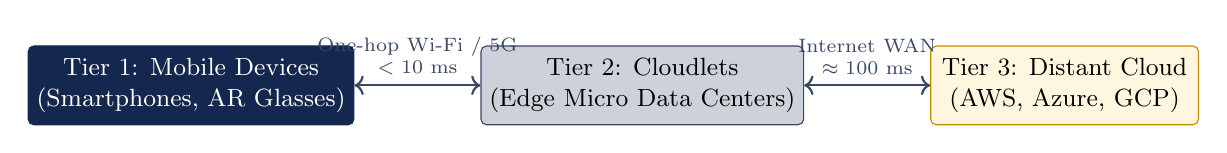
\begin{tikzpicture}[node distance=1.5cm, font=\small]
  \node[dark, minimum width=3.4cm, minimum height=1cm] (tier1) {Tier 1: Mobile Devices\\(Smartphones, AR Glasses)};
  \node[mid, right=1.6cm of tier1, minimum width=3.4cm, minimum height=1cm] (tier2) {Tier 2: Cloudlets\\(Edge Micro Data Centers)};
  \node[gold, right=1.6cm of tier2, minimum width=3.4cm, minimum height=1cm] (tier3) {Tier 3: Distant Cloud\\(AWS, Azure, GCP)};

  \draw[arr, <->] (tier1) -- node[above, font=\scriptsize, align=center] {One-hop Wi-Fi / 5G\\$< 10\text{ ms}$} (tier2);
  \draw[arr, <->] (tier2) -- node[above, font=\scriptsize, align=center] {Internet WAN\\$\approx 100\text{ ms}$} (tier3);
\end{tikzpicture}
\caption{Three-Tier Hierarchy: Mobile Device $\to$ Cloudlet $\to$ Cloud.}
\end{figure}

\begin{defbox}{Cloudlet Definition and Characteristics}
A \textbf{Cloudlet} is a trusted, resource-rich computer or cluster of computers that is well-connected to the Internet and available for use by nearby mobile devices via a high-speed, single-hop wireless local area network (LAN).
\begin{itemize}[leftmargin=*]
  \item \textbf{Zero Administrative Footprint:} Self-managing appliance functioning like a Wi-Fi access point (``data center in a box'').
  \item \textbf{Transient State:} Instantiates temporary virtual machine execution contexts for mobile users and flushes state upon user departure.
  \item \textbf{Dynamic VM Synthesis:} The mobile device transmits a compact, compressed VM overlay (delta) containing application binaries to the cloudlet. The cloudlet rapidly synthesizes the overlay onto a base VM image within seconds.
\end{itemize}
\end{defbox}

\section{Geospatial Cloud Computing}
\subsection{Foundations of Geographic Information Systems (GIS)}
A Geographic Information System (GIS) captures, stores, analyzes, and visualizes spatially referenced data:
\begin{itemize}[leftmargin=*]
  \item \textbf{Vector Data:} Discrete geometric features represented as Points (e.g., GPS tracking coordinates), Lines (e.g., road networks, rivers), and Polygons (e.g., administrative boundaries, parcels).
  \item \textbf{Raster Data:} Continuous gridded pixel arrays representing continuous phenomena (e.g., satellite multispectral imagery, digital elevation models, thermal heat maps).
\end{itemize}

\subsection{Spatial Data Infrastructure (SDI) and OGC Web Standards}
The Open Geospatial Consortium (OGC) establishes open web service specifications for interoperable geospatial cloud platforms:
\begin{center}
\begin{tabularx}{\textwidth}{>{\bfseries}l p{3.5cm} X}
\toprule
OGC Standard & Full Name & Functional Payload and Operation\\
\midrule
WMS & Web Map Service & Renders georeferenced spatial layers into dynamic raster map images (JPEG, PNG) for client display.\\
WFS & Web Feature Service & Queries and returns raw geometric vector features and attribute tables encoded in GML (Geography Markup Language) or GeoJSON.\\
WCS & Web Coverage Service & Delivers raw multidimensional raster coverage data with original sensor values (satellite imagery, DEM grids) for analytical computation.\\
WPS & Web Processing Service & Standardizes inputs and outputs for executing spatial analysis algorithms (e.g., polygon intersection, buffer generation, viewshed analysis) in the cloud.\\
\bottomrule
\end{tabularx}
\end{center}

\subsection{Cloud Scaling for Big Spatial Data}
Geospatial data generation has exploded due to commercial satellite constellations, Earth observation platforms, and ubiquitous mobile smartphone GPS logs. Storing and querying terabytes of spatial geometries in the cloud requires specialized architectures:
\begin{itemize}[leftmargin=*]
  \item \textbf{Spatial Partitioning and Indexing:} Traditional B-trees fail on multi-dimensional spatial coordinates. Geospatial clouds implement:
    \begin{itemize}
      \item \emph{R-Trees / R*-Trees:} Bounding spatial objects within hierarchical Minimum Bounding Boxes (MBR).
      \item \emph{Quadtrees:} Recursive 2D quadrant partitioning of spatial bounding domains.
      \item \emph{GeoHash:} Space-filling Z-order curves that encode 2D latitude-longitude coordinates into 1D alphanumeric strings, allowing spatial proximity range queries inside standard NoSQL Key-Value stores (e.g., Apache HBase, AWS DynamoDB).
    \end{itemize}
  \item \textbf{Distributed Spatial MapReduce:} Splitting spatial datasets across Hadoop clusters where Mapper tasks process spatial tiles in parallel, and Reducers execute spatial joins (e.g., finding all GPS points intersecting a polygonal boundary).
\end{itemize}

\section{Comprehensive Solved Assignment Problems (Week 7)}

\begin{solved}{Unsuitable Workload for Cloud Offloading}
\Given Identify the application least suitable for computation offloading to a remote cloud in MCC.
\Steps
\begin{enumerate}[leftmargin=*]
  \item Image rendering, ML inference, and video transcoding tolerate seconds of delay and benefit from cloud GPUs.
  \item \textbf{Emergency collision avoidance} demands deterministic sub-10 ms response. Network latency, packet jitter, and cellular dropouts make remote cloud offloading dangerous.
\end{enumerate}
\Answer \textbf{Emergency collision avoidance requiring millisecond response}.
\end{solved}

\begin{solved}{Dynamic Resource Scaling Property}
\Given An application automatically provisions additional resources during demand surges and releases them when load drops.
\Steps
\begin{enumerate}[leftmargin=*]
  \item Automated scaling up/down in proportion to dynamic workload demand is the definition of \textbf{Rapid Elasticity}.
\end{enumerate}
\Answer \textbf{Rapid elasticity}.
\end{solved}

\begin{solved}{Dynamic Offloading Optimization Objectives}
\Given Dynamic computation offloading algorithms primarily balance which combination of metrics?
\Steps
\begin{enumerate}[leftmargin=*]
  \item Offloading decisions evaluate execution delay, mobile battery power consumption, and network bandwidth utilization.
\end{enumerate}
\Answer \textbf{Execution time, energy consumption, and resource utilization}.
\end{solved}

\begin{solved}{Low-Latency Infrastructure for Mobile AR}
\Given An augmented reality app requires object recognition with end-to-end response time under 20 ms.
\Steps
\begin{enumerate}[leftmargin=*]
  \item Distant clouds introduce $\ge 100\text{ ms}$ WAN latency.
  \item A nearby \textbf{Cloudlet} reached via single-hop Wi-Fi provides low-latency compute capability within the required 20 ms window.
\end{enumerate}
\Answer \textbf{A nearby cloudlet connected through a high-speed local network}.
\end{solved}

\begin{solved}{Healthcare Cloud Security Requirement}
\Given Which security requirement is paramount to prevent unauthorized access to cloud-hosted medical records?
\Steps
\begin{enumerate}[leftmargin=*]
  \item Preventing unauthorized disclosure of confidential medical records is the core objective of \textbf{Data Confidentiality}.
\end{enumerate}
\Answer \textbf{Data confidentiality}.
\end{solved}

\begin{solved}{Primary Problem Solved by Fog/Edge Computing}
\Given What fundamental limitation of traditional centralized clouds is resolved by fog computing?
\Steps
\begin{enumerate}[leftmargin=*]
  \item Transmitting data to geographically distant hyperscale facilities incurs significant network transit delay. Fog computing places compute near devices to eliminate this \textbf{high network latency}.
\end{enumerate}
\Answer \textbf{High network latency caused by distant cloud data centers}.
\end{solved}

\begin{solved}{Fog Nodes Characteristics Statement Analysis}
\Given Identify the FALSE statement regarding fog nodes.
\Steps
\begin{enumerate}[leftmargin=*]
  \item Fog nodes filter and aggregate sensor data (True).
  \item Fog nodes are positioned close to IoT devices (True).
  \item Fog nodes \emph{permanently store all enterprise data} (FALSE). Fog nodes have limited storage capacity and flush transient data; permanent long-term historical storage resides in the centralized cloud.
\end{enumerate}
\Answer \textbf{They permanently store all enterprise data}.
\end{solved}

\begin{solved}{OGC Service for Vector Geometries}
\Given Which Open Geospatial Consortium service delivers raw vector geographic features (points, lines, polygons)?
\Steps
\begin{enumerate}[leftmargin=*]
  \item WMS returns rendered map images.
  \item \textbf{Web Feature Service (WFS)} delivers raw vector spatial geometry features and attributes.
\end{enumerate}
\Answer \textbf{Web Feature Service (WFS)}.
\end{solved}

\begin{solved}{Offloading Energy Break-Even Condition}
\Given State the algebraic condition under which offloading saves mobile battery energy.
\Steps
\begin{enumerate}[leftmargin=*]
  \item From Kumar and Lu's model, $\Delta E = E_{\text{local}} - E_{\text{cloud}} > 0$.
  \item This directly requires:
  \begin{equation}
  \frac{D}{B} < \frac{C}{M} \left( \frac{P_c - P_i/F}{P_{\text{tr}}} \right)
  \end{equation}
\end{enumerate}
\Answer \textbf{$\frac{D}{B} < \frac{C}{M} \left( \frac{P_c - P_i/F}{P_{\text{tr}}} \right)$}.
\end{solved}

\begin{solved}{Spatial Indexing Primitives in Cloud GIS}
\Given Which spatial indexing mechanism uses recursive 2D space partitioning to index geospatial datasets?
\Steps
\begin{enumerate}[leftmargin=*]
  \item A \textbf{Quadtree} recursively subdivides a two-dimensional spatial region into four quadrants (nodes) to index coordinates efficiently.
\end{enumerate}
\Answer \textbf{Quadtree}.
\end{solved}

% ==================================================================
%  WEEK 8
% ==================================================================
\chapter{Containers, Docker Virtualization, and Sensor-Cloud Infrastructure}

\section{Introduction and Week Overview}
Week 8 transitions from heavy hypervisor-based hardware virtualization into lightweight operating-system-level virtualization (Containers and Docker), followed by the architecture of Sensor-Cloud computing. The key modules examined include:
\begin{enumerate}[leftmargin=*]
  \item \textbf{Containers vs Virtual Machines:} Kernel-sharing mechanics, isolation primitives, architectural tradeoffs, and performance benchmarking.
  \item \textbf{Docker Ecosystem and Architecture:} The Docker engine, copy-on-write image layering (UnionFS/OverlayFS), Dockerfile build directives, and container lifecycle CLI commands.
  \item \textbf{Container Orchestration Primitives:} High-level role of Kubernetes and distributed configuration state management via \texttt{etcd}.
  \item \textbf{Sensor-Cloud Framework:} Bridging Wireless Sensor Networks (WSNs) with cloud elasticity; virtual sensors, multi-tenant provisioning topologies, and layered middleware architectures.
\end{enumerate}

\section{Containers vs Virtual Machines: Architectural Divergence}
\subsection{Structural Comparison}
Traditional virtualization relies on a hypervisor (Type-1 or Type-2) to emulate physical hardware (CPUs, chipsets, network interface cards, memory controllers, BIOS). Each guest Virtual Machine must run a complete, independent guest operating system including its own kernel, device drivers, and system services.

In contrast, \textbf{Operating System-Level Virtualization (Containerization)} relies on kernel-level isolation features within a single host operating system kernel to partition user space into isolated execution environments known as \textbf{Containers}.

\begin{figure}[H]
\centering
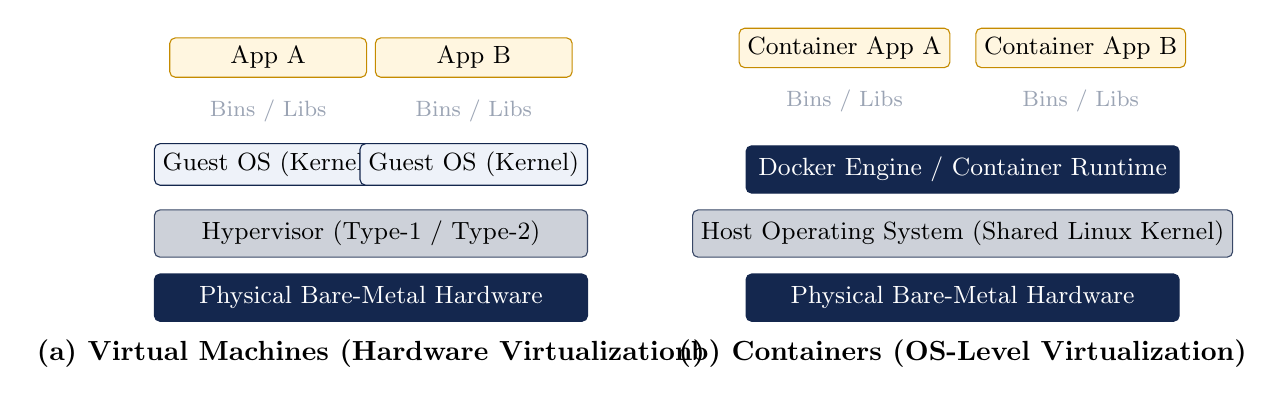
\begin{tikzpicture}[font=\footnotesize]
  % VM Stack
  \node[dark, minimum width=5.5cm, minimum height=0.6cm] (hw1) {Physical Bare-Metal Hardware};
  \node[mid, above=0.2cm of hw1, minimum width=5.5cm, minimum height=0.6cm] (hyp) {Hypervisor (Type-1 / Type-2)};
  
  \node[box, above=0.3cm of hyp.north west, anchor=south west, minimum width=2.5cm, minimum height=0.5cm] (gos1) {Guest OS (Kernel)};
  \node[box, above=0.3cm of hyp.north east, anchor=south east, minimum width=2.5cm, minimum height=0.5cm] (gos2) {Guest OS (Kernel)};
  
  \node[steel, above=0.15cm of gos1, minimum width=2.5cm, minimum height=0.5cm] (bin1) {Bins / Libs};
  \node[steel, above=0.15cm of gos2, minimum width=2.5cm, minimum height=0.5cm] (bin2) {Bins / Libs};
  
  \node[gold, above=0.15cm of bin1, minimum width=2.5cm, minimum height=0.5cm] (app1) {App A};
  \node[gold, above=0.15cm of bin2, minimum width=2.5cm, minimum height=0.5cm] (app2) {App B};

  \node[below=0.1cm of hw1, font=\bfseries] {(a) Virtual Machines (Hardware Virtualization)};

  % Container Stack
  \node[dark, right=2cm of hw1, minimum width=5.5cm, minimum height=0.6cm] (hw2) {Physical Bare-Metal Hardware};
  \node[mid, above=0.2cm of hw2, minimum width=5.5cm, minimum height=0.6cm] (hostos) {Host Operating System (Shared Linux Kernel)};
  \node[dark, above=0.2cm of hostos, minimum width=5.5cm, minimum height=0.6cm] (dockerd) {Docker Engine / Container Runtime};

  \node[steel, above=0.3cm of dockerd.north west, anchor=south west, minimum width=2.5cm, minimum height=0.5cm] (cbin1) {Bins / Libs};
  \node[steel, above=0.3cm of dockerd.north east, anchor=south east, minimum width=2.5cm, minimum height=0.5cm] (cbin2) {Bins / Libs};

  \node[gold, above=0.15cm of cbin1, minimum width=2.5cm, minimum height=0.5cm] (capp1) {Container App A};
  \node[gold, above=0.15cm of cbin2, minimum width=2.5cm, minimum height=0.5cm] (capp2) {Container App B};

  \node[below=0.1cm of hw2, font=\bfseries] {(b) Containers (OS-Level Virtualization)};
\end{tikzpicture}
\caption{Architectural Comparison: Virtual Machines vs Application Containers.}
\end{figure}

\subsection{Quantitative Tradeoff Analysis}
\begin{center}
\begin{tabularx}{\textwidth}{>{\bfseries}l X X}
\toprule
Metric / Dimension & Virtual Machines (VMs) & Containers (Docker)\\
\midrule
Isolation Level & High (Hardware-enforced by MMU, VT-x, and separate kernel ring 0). & Medium-High (Process-level isolation enforced by host kernel namespaces and cgroups).\\
Kernel Instances & Each VM executes its own discrete OS kernel. & All containers share the single host OS kernel.\\
Startup Latency & Minutes ($30\text{ s}$ to $180\text{ s}$) due to full virtual BIOS and OS boot. & Milliseconds to seconds ($< 1\text{ s}$) as processes spawn directly.\\
Disk Footprint & Gigabytes ($2\text{ GB}$ to $40\text{ GB}$) per instance (entire OS image). & Megabytes ($10\text{ MB}$ to $500\text{ MB}$) containing only app dependencies.\\
CPU/RAM Overhead & Significant ($10\%$ to $25\%$) dedicated to running guest OS daemons. & Minimal ($< 1\%$), near bare-metal execution performance.\\
Density & Tens of VMs per physical bare-metal host. & Hundreds to thousands of containers per physical host.\\
Portability & Heavy image formats (VMDK, VHD, QCOW2) tied to hypervisor formats. & Standard OCI image formats portable across any Linux distribution.\\
\bottomrule
\end{tabularx}
\end{center}

\section{The Docker Ecosystem and Architecture}
\subsection{Docker Engine Components}
Docker is an open-source platform that automates the deployment, scaling, and management of applications inside portable container environments. The Docker architecture consists of:
\begin{itemize}[leftmargin=*]
  \item \textbf{Docker Daemon (\texttt{dockerd}):} The persistent background service running on the host that builds images, manages container states, attaches virtual networks, and coordinates storage volumes.
  \item \textbf{Docker Client (\texttt{docker}):} The command-line interface (CLI) tool through which users interact with \texttt{dockerd} via REST API endpoints over UNIX domain sockets (\texttt{/var/run/docker.sock}) or TCP.
  \item \textbf{Docker Images:} Read-only, immutable templates composed of stacked union filesystem layers.
  \item \textbf{Docker Containers:} Runnable instances of a Docker image. When a container starts, a thin, writable copy-on-write (CoW) layer is mounted on top of the immutable image layers.
  \item \textbf{Docker Registry (Docker Hub):} Centralized repositories for publishing, distributing, and pulling container images.
\end{itemize}

\subsection{Copy-on-Write (CoW) and Storage Layering}
Docker utilizes union filesystems (such as \textbf{OverlayFS} or \textbf{AUFS}) to stack directories and present them as a single cohesive unified filesystem:
\begin{itemize}[leftmargin=*]
  \item When multiple containers instantiate the identical base image (\texttt{ubuntu:22.04}), they all share the identical read-only physical disk blocks in memory.
  \item If a container modifies an existing file, the underlying file is copied up from the read-only layer into the container's top-level writable layer before modification (\emph{Copy-on-Write}). This ensures zero mutation of base images.
\end{itemize}

\subsection{Dockerfile Syntax and Construction}
A \textbf{Dockerfile} is a declarative text manifest specifying the sequential instructions required to assemble a Docker image:
\begin{lstlisting}[language=bash]
# Base image layer
FROM python:3.9-slim

# Set execution working directory
WORKDIR /app

# Copy dependency manifest and install packages
COPY requirements.txt .
RUN pip install --no-cache-dir -r requirements.txt

# Copy application source code into image layer
COPY . .

# Expose internal listening port
EXPOSE 5000

# Specify default container entry command
CMD ["python", "app.py"]
\end{lstlisting}

\subsection{Complete Docker Command Lifecycle}
\begin{center}
\begin{tabularx}{\textwidth}{>{\bfseries\ttfamily}l X}
\toprule
Docker Command & Operational Execution Description\\
\midrule
docker build -t myapp:1.0 . & Reads the local Dockerfile, executes instructions sequentially, caches intermediate layers, and tags the resulting image.\\
docker run -d -p 8080:5000 myapp:1.0 & Instantiates a container in detached mode (\texttt{-d}), binding host port 8080 to container port 5000 (\texttt{-p}).\\
docker ps -a & Lists all containers (both actively running and terminated/exited).\\
docker stop <container\_id> & Sends SIGTERM followed by SIGKILL to gracefully terminate container processes.\\
docker rm <container\_id> & Deletes a stopped container instance and purges its writable layer.\\
docker rmi <image\_id> & Permanently deletes an unreferenced container image from the local storage cache.\\
docker network ls & Displays all configured virtual bridge, overlay, and host networks.\\
docker exec -it <id> /bin/bash & Spawns an interactive bash shell session inside an actively running container.\\
\bottomrule
\end{tabularx}
\end{center}

\section{Container Orchestration: Kubernetes and etcd}
When applications scale to thousands of containers spanning hundreds of bare-metal servers, manual container management becomes impossible. \textbf{Kubernetes} automates container scheduling, automated rollouts, service discovery, load balancing, and self-healing.

\begin{defbox}{Role of \texttt{etcd} in Kubernetes Clusters}
\textbf{\texttt{etcd}} is a strongly consistent, distributed, and highly available key-value datastore based on the \textbf{Raft consensus algorithm}.\\
In Kubernetes, \texttt{etcd} serves as the ultimate single source of truth for the entire cluster. It persistently stores:
\begin{itemize}[leftmargin=*]
  \item Cluster configuration states, namespaces, and node registrations.
  \item Pod definitions, ReplicaSets, and Deployments.
  \item Secrets, ConfigMaps, and cluster metadata.
\end{itemize}
The Kubernetes control plane components (API Server, Scheduler, Controller Manager) are stateless; they coordinate state transitions strictly by reading from and writing to \texttt{etcd}.
\end{defbox}

\section{Sensor-Cloud Infrastructure}
\subsection{Limitations of Traditional Wireless Sensor Networks (WSNs)}
Traditional Wireless Sensor Networks (WSNs) consist of small sensor motes deployed to monitor physical environments (temperature, moisture, seismic activity). However, conventional WSNs exhibit severe structural limitations:
\begin{itemize}[leftmargin=*]
  \item \textbf{Isolated Application Silos:} A sensor network deployed for soil moisture monitoring is typically accessible only to a single proprietary backend application.
  \item \textbf{Resource Exhaustion:} Sensor nodes possess limited battery life, micro-controllers with few kilobytes of RAM, and low-power radios.
  \item \textbf{No Multi-Tenancy:} Multiple users with differing analytical queries cannot dynamically share the same physical sensor hardware simultaneously.
\end{itemize}

\subsection{The Sensor-Cloud Paradigm}
\begin{defbox}{Sensor-Cloud Definition}
\textbf{Sensor-Cloud} is an infrastructure that virtualizes physical Wireless Sensor Networks into dynamically manageable, reconfigurable, and multi-tenant \textbf{Virtual Sensors} provisioned on-demand over the cloud.
\end{defbox}

\begin{figure}[H]
\centering
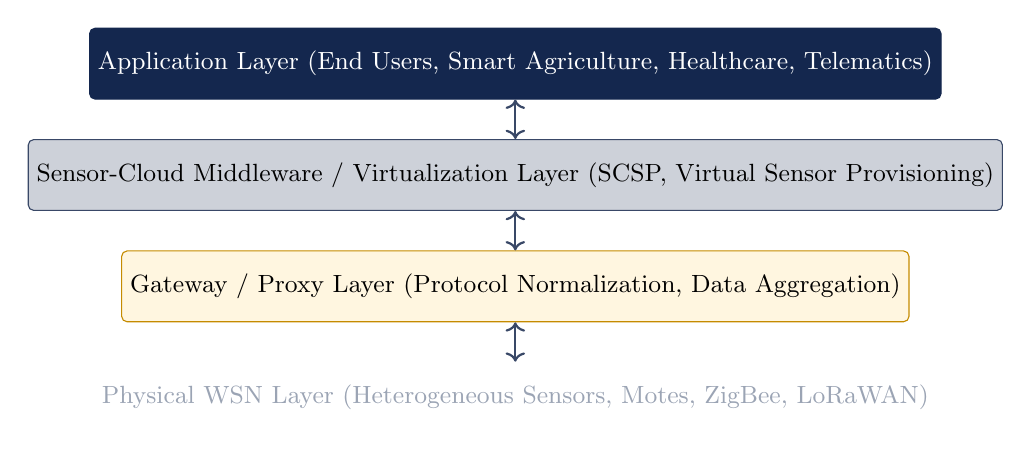
\begin{tikzpicture}[node distance=1.2cm, font=\small]
  % Layers
  \node[dark, minimum width=10cm, minimum height=0.9cm] (app) {Application Layer (End Users, Smart Agriculture, Healthcare, Telematics)};
  \node[mid, below=0.5cm of app, minimum width=10cm, minimum height=0.9cm] (scsp) {Sensor-Cloud Middleware / Virtualization Layer (SCSP, Virtual Sensor Provisioning)};
  \node[gold, below=0.5cm of scsp, minimum width=10cm, minimum height=0.9cm] (gw) {Gateway / Proxy Layer (Protocol Normalization, Data Aggregation)};
  \node[steel, below=0.5cm of gw, minimum width=10cm, minimum height=0.9cm] (wsn) {Physical WSN Layer (Heterogeneous Sensors, Motes, ZigBee, LoRaWAN)};

  \draw[arr, <->] (app) -- (scsp);
  \draw[arr, <->] (scsp) -- (gw);
  \draw[arr, <->] (gw) -- (wsn);
\end{tikzpicture}
\caption{Layered Architecture of Sensor-Cloud Computing.}
\end{figure}

\subsection{Stakeholders and Economic Model}
Sensor-Cloud establishes a three-party multi-tenant marketplace:
\begin{enumerate}[leftmargin=*]
  \item \textbf{Physical Sensor Owners:} Entities that procure and deploy physical sensor hardware in the field. They register their WSNs with the Sensor-Cloud provider to monetize idle sensing capacity.
  \item \textbf{Sensor-Cloud Service Provider (SCSP):} The cloud entity that maintains the virtualization middleware, registers physical sensors, provisions virtual sensors, negotiates SLAs, and handles metering and billing.
  \item \textbf{End Users:} Consumers or enterprises who provision virtual sensors on-demand for specific temporal durations and geographic boundaries without purchasing physical hardware.
\end{enumerate}

\subsection{Virtual Sensor Configurations and Mapping Topologies}
A \textbf{Virtual Sensor} is a software abstraction representing a sensing unit provisioned in the cloud. It decouples the user application from the underlying physical sensor hardware. The virtualization engine supports three primary configurations:

\begin{itemize}[leftmargin=*]
  \item \textbf{One-to-One Mapping ($1:1$):} A single virtual sensor directly represents a single physical sensor mote.
  \item \textbf{Many-to-One Mapping ($N:1$):} Multiple physical sensor motes are aggregated into a single virtual sensor. For example, averaging temperature readings from 20 distributed agricultural sensor nodes across a field into a single virtual temperature feed.
  \item \textbf{One-to-Many Mapping ($1:N$):} A single high-capability physical sensor is dynamically partitioned into multiple virtual sensors serving different end users simultaneously with distinct sampling frequencies and delivery thresholds.
  \item \textbf{Spatio-Temporal Virtual Sensors:} Virtual sensors synthesized dynamically to cover an arbitrary geographical polygon $\mathcal{R}$ over a designated time window $[t_1, t_2]$, collecting and synthesizing telemetry from all physical sensors falling inside $\mathcal{R}$.
\end{itemize}

\section{Comprehensive Solved Assignment Problems (Week 8)}

\begin{solved}{Docker Image Deletion Command}
\Given Which command deletes a Docker image that is no longer required?
\Steps
\begin{enumerate}[leftmargin=*]
  \item \texttt{docker rm} removes stopped \emph{containers}.
  \item \texttt{docker rmi} (\textbf{r}e\textbf{m}ove \textbf{i}mage) purges container \emph{images}.
\end{enumerate}
\Answer \textbf{\texttt{docker rmi}}.
\end{solved}

\begin{solved}{Listing Docker Virtual Networks}
\Given Identify the command used to display all available Docker networks on the host.
\Steps
\begin{enumerate}[leftmargin=*]
  \item Docker CLI manages network namespaces via the \texttt{network} command group.
  \item The command \texttt{docker network ls} lists all bridge, host, and overlay networks.
\end{enumerate}
\Answer \textbf{\texttt{docker network ls}}.
\end{solved}

\begin{solved}{VM vs Container Kernel Isolation Comparison}
\Given Which is the most accurate comparison between VMs and containers?
\Steps
\begin{enumerate}[leftmargin=*]
  \item Virtual Machines virtualize physical hardware, executing complete guest operating systems with independent kernels.
  \item Containers share the underlying host OS kernel, providing process isolation via Linux kernel namespaces and cgroups.
\end{enumerate}
\Answer \textbf{Containers generally share the host kernel, while VMs virtualize hardware and run separate guest OS kernels}.
\end{solved}

\begin{solved}{Primary Function of etcd in Kubernetes}
\Given What is the fundamental responsibility of \texttt{etcd} in a Kubernetes cluster?
\Steps
\begin{enumerate}[leftmargin=*]
  \item \texttt{etcd} is a distributed key-value store used to persist cluster configuration data, metadata, and state information across all master control plane components.
\end{enumerate}
\Answer \textbf{Storing Kubernetes cluster state and configuration data}.
\end{solved}

\begin{solved}{Hypervisor Type Classification}
\Given Identify an example of a Type 2 (hosted) hypervisor among: VMware ESXi, Xen, Oracle VirtualBox, Microsoft Hyper-V Server.
\Steps
\begin{enumerate}[leftmargin=*]
  \item VMware ESXi, Xen, and Hyper-V Server are Type-1 bare-metal hypervisors.
  \item \textbf{Oracle VirtualBox} runs as an application process on top of a standard host operating system (Windows, Linux, macOS), making it a Type 2 hypervisor.
\end{enumerate}
\Answer \textbf{Oracle VirtualBox}.
\end{solved}

\begin{solved}{Energy Reduction via VM Consolidation}
\Given In a data center of 100 servers, 40 are heavily loaded while 60 operate at very low utilization. What is the most effective energy saving strategy?
\Steps
\begin{enumerate}[leftmargin=*]
  \item Idle servers consume $50\%$ to $60\%$ of peak power.
  \item Consolidating VMs from underutilized servers onto fewer hosts via live migration allows the empty physical machines to be powered down into sleep states, maximizing energy savings.
\end{enumerate}
\Answer \textbf{Consolidate VMs onto fewer servers and switch idle servers to a low-power state}.
\end{solved}

\begin{solved}{Role of Middleware in Sensor-Cloud}
\Given Why is a middleware layer required between Wireless Sensor Networks (WSNs) and cloud applications?
\Steps
\begin{enumerate}[leftmargin=*]
  \item Physical sensor motes use diverse, proprietary communication protocols and data formats.
  \item The middleware abstracts heterogeneous physical sensors, enabling cloud-accessible virtual sensors with standardized APIs.
\end{enumerate}
\Answer \textbf{To abstract heterogeneous sensors and provide cloud-accessible sensor resources}.
\end{solved}

\begin{solved}{Virtual Sensor Provisioning Topologies}
\Given Can multiple physical sensors be aggregated to form a single virtual sensor?
\Steps
\begin{enumerate}[leftmargin=*]
  \item Yes, Sensor-Cloud supports Many-to-One ($N:1$) mapping, allowing data from multiple geographic sensors to be aggregated into a single virtual sensor feed.
\end{enumerate}
\Answer \textbf{Yes, Many-to-One mapping is supported}.
\end{solved}

\begin{solved}{Docker Container Isolation Primitives}
\Given Which Linux kernel primitives provide resource metering and process isolation for Docker containers?
\Steps
\begin{enumerate}[leftmargin=*]
  \item \textbf{Namespaces} partition system resources (process IDs, network interfaces, mount points).
  \item \textbf{Control Groups (cgroups)} meter and limit hardware consumption (CPU shares, memory quotas, I/O bandwidth).
\end{enumerate}
\Answer \textbf{Namespaces and cgroups}.
\end{solved}

\begin{solved}{Economic Benefit of Sensor-Cloud to Sensor Owners}
\Given How do physical sensor owners benefit economically in the Sensor-Cloud model?
\Steps
\begin{enumerate}[leftmargin=*]
  \item Sensor owners register their physical WSNs with the Sensor-Cloud Service Provider (SCSP) and earn recurring revenue from multi-tenant subscriptions without building custom software applications.
\end{enumerate}
\Answer \textbf{Monetizing deployed physical sensor capacity through multi-tenant usage fees}.
\end{solved}

% ==================================================================
%  WEEK 9
% ==================================================================
\chapter{Hierarchical Edge-Fog-Cloud Computing and Cloud Federation}

\section{Introduction and Week Overview}
Week 9 explores the continuum between centralized hyperscale data centers and decentralized edge computing. Centralized clouds struggle to process the massive volume, velocity, and variety of data generated by billions of Internet of Things (IoT) devices with low latency. This module covers:
\begin{enumerate}[leftmargin=*]
  \item \textbf{The Edge-Fog-Cloud Continuum:} Cisco's Fog Computing architectural paradigm, multi-tier hierarchical delegation, and latency-sensitive control loops.
  \item \textbf{Empirical Performance Modeling with iFogSim:} Network bandwidth conservation, execution cost reduction, latency bounds, and healthcare case studies.
  \item \textbf{Resource Management and Service Placement:} Formal taxonomies of resource management (Data Flow, Control, Tenancy), vertical vs horizontal scalability, and multi-objective task placement.
  \item \textbf{Cloud Federation and Inter-Cloud Governance:} Overcoming vendor lock-in through Broker Architectures, Peer-to-Peer (P2P) peering, and cross-provider SLA enforcement.
\end{enumerate}

\section{The Edge-Fog-Cloud Computing Hierarchy}
\subsection{The Need for Decentralization}
While hyperscale cloud computing provides elastic computing capacity and virtually infinite storage, routing all raw IoT telemetry to centralized data centers introduces critical bottlenecks:
\begin{itemize}[leftmargin=*]
  \item \textbf{Excessive WAN Latency:} Multi-hop packet routing across public Internet backbones introduces unpredictable delays ($100\text{ ms}$ to $300\text{ ms}$), violating real-time cyber-physical feedback loops.
  \item \textbf{Core Network Congestion:} Streaming millions of high-definition video feeds or high-frequency vibrational sensor telemetry overloads Internet Service Provider (ISP) backbones.
  \item \textbf{Data Privacy and Sovereignty:} Raw audio, video, and biometric streams transmitted across national borders pose regulatory and privacy risks.
\end{itemize}

\subsection{Architectural Division of Responsibilities}
Introduced by Cisco Systems and formalized in IEEE/ACM distributed systems research, the \textbf{Edge--Fog--Cloud} hierarchy divides responsibilities across three distinct tiers:

\begin{figure}[H]
\centering
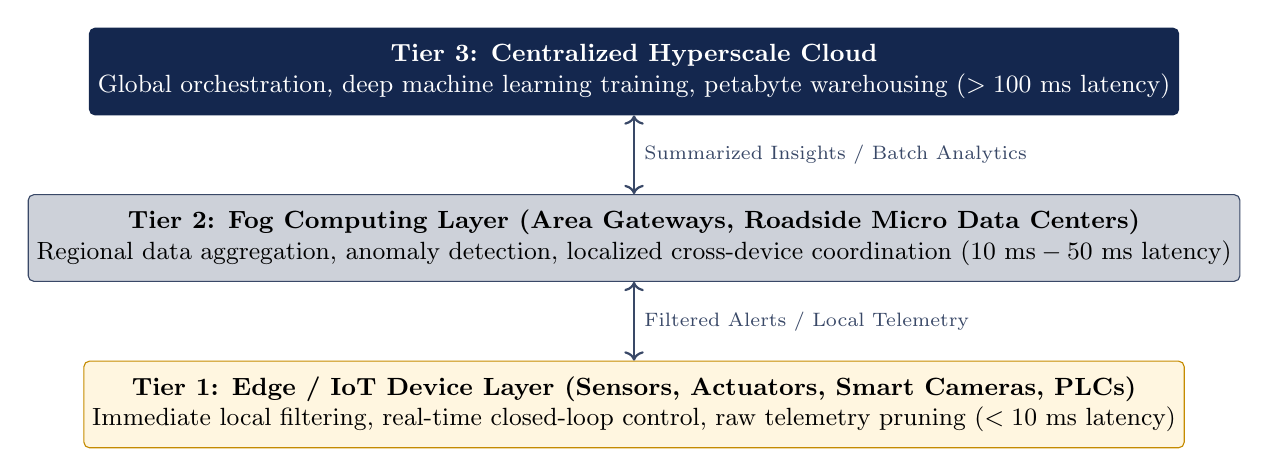
\begin{tikzpicture}[font=\small]
  % Cloud Tier
  \node[dark, minimum width=12cm, minimum height=1.1cm] (cloud) {\textbf{Tier 3: Centralized Hyperscale Cloud}\\Global orchestration, deep machine learning training, petabyte warehousing ($> 100\text{ ms}$ latency)};
  
  % Fog Tier
  \node[mid, below=1cm of cloud, minimum width=12cm, minimum height=1.1cm] (fog) {\textbf{Tier 2: Fog Computing Layer (Area Gateways, Roadside Micro Data Centers)}\\Regional data aggregation, anomaly detection, localized cross-device coordination ($10\text{ ms} - 50\text{ ms}$ latency)};
  
  % Edge Tier
  \node[gold, below=1cm of fog, minimum width=12cm, minimum height=1.1cm] (edge) {\textbf{Tier 1: Edge / IoT Device Layer (Sensors, Actuators, Smart Cameras, PLCs)}\\Immediate local filtering, real-time closed-loop control, raw telemetry pruning ($< 10\text{ ms}$ latency)};

  \draw[arr, <->] (cloud) -- node[right, font=\scriptsize] {Summarized Insights / Batch Analytics} (fog);
  \draw[arr, <->] (fog) -- node[right, font=\scriptsize] {Filtered Alerts / Local Telemetry} (edge);
\end{tikzpicture}
\caption{Three-Tier Edge-Fog-Cloud Hierarchical Architecture.}
\end{figure}

\begin{center}
\begin{tabularx}{\textwidth}{>{\bfseries}l X X X}
\toprule
System Dimension & Edge Layer & Fog Layer & Cloud Layer\\
\midrule
Response Latency & Ultra-low ($1\text{ ms} - 10\text{ ms}$) & Low ($10\text{ ms} - 50\text{ ms}$) & Moderate to High ($100\text{ ms} - 500\text{ ms}$)\\
Data Scope & Transient, sensor-local & Regional, facility-wide & Global, enterprise-wide\\
Storage Duration & Seconds (transient buffer) & Hours to days & Years (permanent historical archival)\\
Compute Hardware & Microcontrollers, ASICs, Raspberry Pi & Micro-servers, edge gateways, high-end routers & Multi-socket server blades, GPU clusters\\
Data Volume Flow & Ingests $100\%$ of raw telemetry & Filters/aggregates to $\approx 10\%$ of raw data & Receives $< 1\%$ (compact statistical summaries)\\
Network Uplink & Local Wi-Fi, BLE, ZigBee & Regional Ethernet, 5G NR, Fiber & Transoceanic Internet WAN fiber\\
\bottomrule
\end{tabularx}
\end{center}

\subsection{Empirical Simulation Analysis: The iFogSim Framework}
The lecture features research co-authored by Prof. Soumya K. Ghosh and Prof. Rajkumar Buyya utilizing \textbf{iFogSim}, an open-source Java simulation toolkit for modeling resource management in IoT, Edge, and Fog environments:

\subsubsection{Healthcare Case Study: Smart Ambient Assisted Living}
A patient monitoring application measures ECG, blood pressure, and pulse telemetry:
\begin{itemize}[leftmargin=*]
  \item \textbf{Configuration A (Cloud-Only):} Every raw biometric pulse packet is forwarded directly to AWS cloud servers.
  \item \textbf{Configuration B (Cloud-Fog-Edge):} Wearable edge sensors execute lightweight feature extraction. An Area Gateway (Fog Node) runs automated arrhythmia detection algorithms locally. Only abnormal readings trigger an alert that contacts the cloud confirmatory module.
\end{itemize}

\subsubsection{Performance Findings}
\begin{enumerate}[leftmargin=*]
  \item \textbf{Network Bandwidth Consumption:} In the Fog configuration, network usage decreases by over $90\%$ because raw sinusoidal signals are evaluated locally; only verified anomaly events traverse the wide-area network.
  \item \textbf{Operational Execution Cost:} Cloud compute hours are strictly pay-per-use. Processing raw data on customer-owned edge gateways slashes recurring monthly cloud billing fees.
  \item \textbf{Control Loop Latency:} In the Cloud-only model, closed-loop actuation delays fluctuated between $1500\text{ ms}$ and $4000\text{ ms}$ due to network congestion. In the Fog architecture, control loop latency remained deterministic and fixed below $50\text{ ms}$.
\end{enumerate}

\section{Resource Management and Scalability Models}
\subsection{Resource Management Taxonomies}
Following the ACM survey by Hong and Varghese highlighted in the lecture, resource management in Fog/Edge computing is partitioned along three axes:
\begin{itemize}[leftmargin=*]
  \item \textbf{Data Flow:} Movement of workloads and telemetry. Workloads may flow upstream (from sensor devices to edge/cloud) or downstream (offloading pre-trained AI weights from cloud to edge inferencing engines).
  \item \textbf{Control Hierarchy:}
    \begin{itemize}
      \item \emph{Centralized Control:} A master coordinator governs scheduling across all edge devices.
      \item \emph{Distributed / Autonomous Control:} Edge and fog nodes negotiate tasks peer-to-peer using localized game theory or consensus algorithms.
    \end{itemize}
  \item \textbf{Tenancy:} Single-tenant dedicated hardware vs multi-tenant virtualized containers running concurrent multi-user tasks.
\end{itemize}

\subsection{Vertical vs Horizontal Scalability}
When a computing node experiences resource exhaustion:
\begin{defbox}{Vertical Scalability (Scale-Up) vs Horizontal Scalability (Scale-Out)}
\textbf{Vertical Scalability (Scale-Up):} Increasing the physical or virtual capacity of an existing node by assigning additional CPU cores, expanding system RAM, or upgrading disk I/O throughput within the same machine.\\
\textbf{Horizontal Scalability (Scale-Out):} Adding new independent nodes or servers into the computing pool and distributing incoming workload requests across the expanded cluster via a load balancer.
\end{defbox}

\section{Cloud Federation and Inter-Cloud Governance}
\subsection{Motivation for Cloud Federation}
Relying on a single Cloud Service Provider (CSP) exposes enterprises to catastrophic risks:
\begin{itemize}[leftmargin=*]
  \item \textbf{Vendor Lock-In:} Proprietary APIs, incompatible storage schemas, and exorbitant egress bandwidth fees trap enterprise applications.
  \item \textbf{Geographic Blackouts:} Outages in a single provider's regional data center can incapacitate global business operations.
  \item \textbf{Capacity Exhaustion:} Sudden global demand spikes can surpass a single provider's available unallocated capacity.
\end{itemize}

\begin{defbox}{Cloud Federation}
\textbf{Cloud Federation} is the seamless aggregation and dynamic coordination of computing, storage, and networking resources from multiple autonomous, heterogeneous Cloud Service Providers to satisfy consumer requirements under a unified SLA.
\end{defbox}

\subsection{Federation Architectural Topologies}
\begin{figure}[H]
\centering
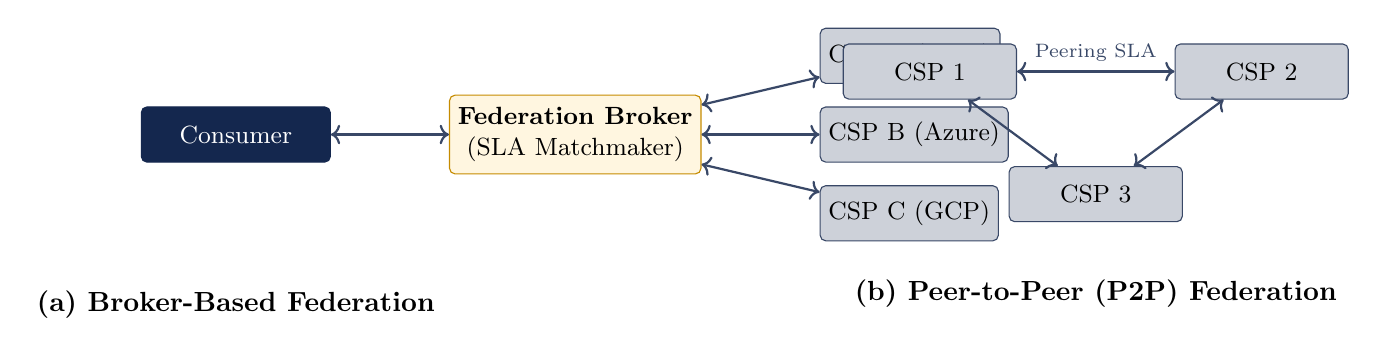
\begin{tikzpicture}[font=\small]
  % Broker Model
  \node[dark, minimum width=2.4cm] (c1) {Consumer};
  \node[gold, right=1.5cm of c1, minimum width=2.8cm, minimum height=1cm] (broker) {\textbf{Federation Broker}\\(SLA Matchmaker)};
  \node[mid, right=1.5cm of broker, yshift=1cm, minimum width=2.2cm] (csp1) {CSP A (AWS)};
  \node[mid, right=1.5cm of broker, minimum width=2.2cm] (csp2) {CSP B (Azure)};
  \node[mid, right=1.5cm of broker, yshift=-1cm, minimum width=2.2cm] (csp3) {CSP C (GCP)};

  \draw[arr, <->] (c1) -- (broker);
  \draw[arr, <->] (broker) -- (csp1);
  \draw[arr, <->] (broker) -- (csp2);
  \draw[arr, <->] (broker) -- (csp3);

  \node[below=1.5cm of c1, font=\bfseries] {(a) Broker-Based Federation};

  % P2P Model
  \node[mid, right=6.5cm of c1, yshift=0.8cm, minimum width=2.2cm] (p1) {CSP 1};
  \node[mid, right=2cm of p1, minimum width=2.2cm] (p2) {CSP 2};
  \node[mid, below=1.2cm of $(p1)!0.5!(p2)$, minimum width=2.2cm] (p3) {CSP 3};

  \draw[arr, <->] (p1) -- node[above, font=\scriptsize] {Peering SLA} (p2);
  \draw[arr, <->] (p2) -- (p3);
  \draw[arr, <->] (p3) -- (p1);

  \node[below=0.6cm of p3, font=\bfseries] {(b) Peer-to-Peer (P2P) Federation};
\end{tikzpicture}
\caption{Architectural Models of Cloud Federation.}
\end{figure}

\begin{enumerate}[leftmargin=*]
  \item \textbf{Broker Architecture (Centralized Federation):} An independent entity (the Cloud Federation Broker) acts as a neutral intermediary between cloud consumers and multiple CSPs:
    \begin{itemize}
      \item Discovers available capacity and catalogs service pricing across diverse providers.
      \item Evaluates consumer QoS and latency constraints, selecting the optimal provider.
      \item Negotiates multi-provider contractual SLAs and orchestrates cross-cloud billing.
    \end{itemize}
  \item \textbf{Peer-to-Peer (P2P) Federation:} Cloud service providers negotiate direct peering agreements without a central broker. When Provider A experiences localized capacity exhaustion, it transparently subcontracts surplus workload to Provider B under pre-agreed bilateral cross-charging tariffs.
\end{enumerate}

\section{Comprehensive Solved Assignment Problems (Week 9)}

\begin{solved}{Multi-Tier Placement for Industrial Anomaly Detection}
\Given A factory requires machine-level anomaly detection within milliseconds and plant-wide data aggregation before sending summaries to the cloud. What is the optimal placement?
\Steps
\begin{enumerate}[leftmargin=*]
  \item Millisecond anomaly detection on individual machines requires processing at the \textbf{Edge}.
  \item Plant-wide aggregation across multiple machines requires intermediate coordination at \textbf{Fog} nodes.
  \item Final long-term historical reporting is handled in the \textbf{Cloud}.
\end{enumerate}
\Answer \textbf{Machine-level processing at the edge and plant-level processing at fog nodes}.
\end{solved}

\begin{solved}{Smart City Multi-Tier Video Analytics Architecture}
\Given Object detection occurs near cameras, regional congestion patterns are analyzed at roadside micro-datacenters, and long-term city trends are processed in the cloud. Which architecture represents this system?
\Steps
\begin{enumerate}[leftmargin=*]
  \item Processing near cameras $\to$ Edge.
  \item Roadside micro-datacenters $\to$ Fog.
  \item Long-term trends in the central facility $\to$ Cloud.
  \item The complete multi-tiered paradigm is \textbf{Edge--Fog--Cloud}.
\end{enumerate}
\Answer \textbf{Edge--Fog--Cloud architecture}.
\end{solved}

\begin{solved}{Raw Data Volume Transmitted to Central Infrastructure}
\Given Rank the architectural strategies by raw data volume transmitted toward the central cloud, from lowest to highest.
\Steps
\begin{enumerate}[leftmargin=*]
  \item \textbf{Edge processing} filters and prunes telemetry immediately at the sensor, transmitting the least volume.
  \item \textbf{Fog processing} aggregates data across a local area, transmitting moderate volume.
  \item \textbf{Cloud-only processing} streams all raw uncompressed data over the WAN, transmitting the highest volume.
\end{enumerate}
\Answer \textbf{Edge processing $\to$ Fog processing $\to$ Cloud-only processing}.
\end{solved}

\begin{solved}{Scaling Mechanism Classification}
\Given A fog node running low on memory is provisioned additional RAM and CPU cores on that same physical machine. Which scalability approach is this?
\Steps
\begin{enumerate}[leftmargin=*]
  \item Upgrading the CPU and RAM capacity of an existing machine without adding new nodes is \textbf{Vertical Scalability} (Scale-Up).
\end{enumerate}
\Answer \textbf{Vertical scalability}.
\end{solved}

\begin{solved}{Division of Responsibilities in Edge-Fog-Cloud}
\Given Which statement best describes the division of responsibilities in a hierarchical Edge-Fog-Cloud system?
\Steps
\begin{enumerate}[leftmargin=*]
  \item Edge executes immediate local actions.
  \item Fog coordinates regional resources and aggregates telemetry.
  \item Cloud performs global optimization and long-term strategic analytics.
\end{enumerate}
\Answer \textbf{Edge handles immediate local actions, Fog coordinates regional resources, and Cloud performs global orchestration}.
\end{solved}

\begin{solved}{Split Architecture for Video Analytics}
\Given A video analytics application requires first-stage inference within 10 ms of the camera, while heavy model retraining requires massive computing power.
\Steps
\begin{enumerate}[leftmargin=*]
  \item Sub-10 ms inference must run at the Edge/Fog close to the camera.
  \item Heavy model training runs in the centralized Cloud.
\end{enumerate}
\Answer \textbf{First-stage inference on an edge/fog node and model training in the cloud}.
\end{solved}

\begin{solved}{Federation Broker Responsibilities}
\Given What is the primary role of a Cloud Federation Broker?
\Steps
\begin{enumerate}[leftmargin=*]
  \item The Federation Broker mediates between consumers and multiple CSPs, discovering available resources, matching SLA terms, and routing workloads across cloud providers.
\end{enumerate}
\Answer \textbf{Discovers, negotiates, and coordinates services across multiple independent cloud providers}.
\end{solved}

\begin{solved}{Limitation of Edge Devices in Heavy Analytics}
\Given Why can't edge devices replace centralized cloud data centers for large-scale historical model training?
\Steps
\begin{enumerate}[leftmargin=*]
  \item Edge devices have constrained CPU, GPU, memory, and battery capacity, making them incapable of processing multi-terabyte datasets required for model training.
\end{enumerate}
\Answer \textbf{Edge devices possess limited computational power, memory, and storage capacity}.
\end{solved}

\begin{solved}{Peer-to-Peer vs Broker Federation}
\Given In a Peer-to-Peer (P2P) cloud federation model, how are resources negotiated?
\Steps
\begin{enumerate}[leftmargin=*]
  \item Participating cloud providers establish direct, bilateral peering agreements to share surplus capacity without relying on a centralized intermediary broker.
\end{enumerate}
\Answer \textbf{Directly between participating cloud providers through bilateral peering agreements}.
\end{solved}

\begin{solved}{Bandwidth Conservation via Fog Preprocessing}
\Given How does fog preprocessing conserve WAN network bandwidth?
\Steps
\begin{enumerate}[leftmargin=*]
  \item By filtering, aggregating, and compressing raw sensor streams locally, preventing redundant telemetry from being transmitted across the core Internet backbone.
\end{enumerate}
\Answer \textbf{By filtering and aggregating telemetry locally before wide-area transmission}.
\end{solved}

% ==================================================================
%  WEEK 10
% ==================================================================
\chapter{Virtual Machine Migration, Container Primitives, and Cloud Orchestration}

\section{Introduction and Week Overview}
Week 10 concludes the technical core of the NPTEL Cloud Computing curriculum by investigating dynamic runtime relocation of compute instances and the deep operating-system primitives governing modern container engines. The curriculum covers:
\begin{enumerate}[leftmargin=*]
  \item \textbf{Virtual Machine Migration Taxonomy:} Motivations (load balancing, hardware maintenance, energy consolidation, fault tolerance), what to migrate (CPU state, memory pages, network connections, storage), and Cold vs Live migration.
  \item \textbf{Live Migration Paradigms:}
    \begin{itemize}
      \item \emph{Pre-Copy Iterative Migration:} Push phase, iterative dirty-page tracking, mathematical convergence criteria ($D < R$), and stop-and-copy downtime.
      \item \emph{Post-Copy Migration:} Rapid CPU context handover, target-first execution, and on-demand network page faulting (Pull phase).
    \end{itemize}
  \item \textbf{Linux Kernel Container Primitives:} The deep mechanics of Linux Namespaces (process isolation) versus Control Groups / cgroups (resource quotas and metering).
  \item \textbf{Docker Storage Persistence:} Ephemeral writable layers vs Docker Named Volumes.
\end{enumerate}

\section{Virtual Machine Migration Fundamentals}
\subsection{Motivation and Operational Drivers}
In a production cloud data center, virtual machines cannot remain permanently pinned to a single physical blade. Dynamic instance relocation is required for:
\begin{itemize}[leftmargin=*]
  \item \textbf{Dynamic Load Balancing:} Relieving resource congestion when a physical server experiences CPU, RAM, or I/O saturation.
  \item \textbf{Zero-Downtime Hardware Maintenance:} Evacuating all active tenant VMs from a physical server prior to hardware upgrades, firmware flashes, or operating system patches.
  \item \textbf{Green Energy Consolidation:} Packing lightly loaded VMs onto fewer physical servers during off-peak hours and powering off redundant hosts into low-power ACPI sleep states.
  \item \textbf{Proactive Fault Tolerance:} Migrating VMs away from hardware nodes exhibiting escalating memory ECC error rates or thermal warnings before fatal crashes occur.
\end{itemize}

\subsection{The Migration State Tuple}
A virtual machine is fully encapsulated as a state tuple:
\begin{equation}
\mathcal{S}_{\text{VM}} = \langle \mathcal{C}_{\text{CPU}}, \mathcal{M}_{\text{RAM}}, \mathcal{D}_{\text{Storage}}, \mathcal{N}_{\text{Network}}, \mathcal{I}_{\text{I/O}} \rangle
\end{equation}
\begin{itemize}[leftmargin=*]
  \item \textbf{CPU Context ($\mathcal{C}_{\text{CPU}}$):} Register states, Program Counter (PC), translation lookaside buffer (TLB) state, and virtual interrupt controllers. Size: Kilobytes; transfer time: milliseconds.
  \item \textbf{Main Memory ($\mathcal{M}_{\text{RAM}}$):} The entire physical memory space allocated to the guest OS ($2\text{ GB}$ to $512\text{ GB}$). Migrating active memory while guest processes continuously modify memory pages is the central algorithmic challenge of live migration.
  \item \textbf{Persistent Storage ($\mathcal{D}_{\text{Storage}}$):} In enterprise clouds, storage disks reside on shared network-attached storage (NAS, SAN, or Ceph). The virtual disk is accessible from both source and destination physical hosts, avoiding the need to transfer multi-terabyte disk images across the migration link.
  \item \textbf{Network State ($\mathcal{N}_{\text{Network}}$):} The VM must retain its IP address and open TCP connections. Upon migration completion to a new switch port, the target hypervisor emits a \textbf{Gratuitous ARP (GARP)} broadcast, updating network switch forwarding tables (CAM tables) without severing established client sessions.
\end{itemize}

\section{Cold vs Live Migration Taxonomy}
\begin{center}
\begin{tabularx}{\textwidth}{>{\bfseries}l X X}
\toprule
Dimension & Cold (Offline / Non-Live) Migration & Live (Hot / Online) Migration\\
\midrule
VM State During Transfer & Powered off, halted, or suspended. & Actively running and processing user requests.\\
Service Downtime & Long ($T_{\text{downtime}} = T_{\text{transfer}}$). Equal to total migration duration. & Near-zero ($T_{\text{downtime}} \ll T_{\text{transfer}}$), typically $50\text{ ms} - 500\text{ ms}$.\\
Implementation Complexity & Trivial (copy memory/disk snapshot file and boot on target). & High (requires continuous dirty-page tracking or on-demand page pulling).\\
Application Impact & Unacceptable for latency-sensitive, real-time, or transactional services. & Undetectable by end users and active TCP sessions.\\
\bottomrule
\end{tabularx}
\end{center}

\subsection{Cold Migration Transfer Duration Formulation}
In cold migration, the entire memory footprint $V_m$ must be transferred over a network connection with usable sustained throughput $R$:
\begin{equation}
T_{\text{transfer}} = \frac{V_m}{R}
\end{equation}

\begin{solved}{Cold VM Migration Duration Calculation}
\Given A virtual machine has memory $V_m = 32\text{ GB}$. The migration link provides a sustained throughput $R = 16\text{ MB/s}$. Calculate the transfer duration for a non-live migration. (Use $1\text{ GB} = 2^{30}\text{ bytes}$, $1\text{ MB} = 2^{20}\text{ bytes}$).
\Formula
\begin{equation}
T = \frac{V_m}{R}
\end{equation}
\Steps
\begin{enumerate}[leftmargin=*]
  \item Convert gigabytes to megabytes:
  \begin{equation}
  V_m = 32\text{ GB} = 32 \times 1024\text{ MB} = 32,768\text{ MB}
  \end{equation}
  \item Compute duration in seconds:
  \begin{equation}
  T = \frac{32,768\text{ MB}}{16\text{ MB/s}} = 2048\text{ seconds}
  \end{equation}
  \item Convert to minutes:
  \begin{equation}
  T_{\text{minutes}} = \frac{2048}{60} \approx 34.133\text{ minutes} \quad (\approx 34\text{ minutes})
  \end{equation}
\end{enumerate}
\Answer The transfer duration is approximately \textbf{34 minutes} ($2048$ seconds).
\end{solved}

\section{Live Migration Paradigms: Pre-Copy vs Post-Copy}
Live migration decouples total migration time from service downtime through two primary algorithmic strategies:

\begin{figure}[H]
\centering
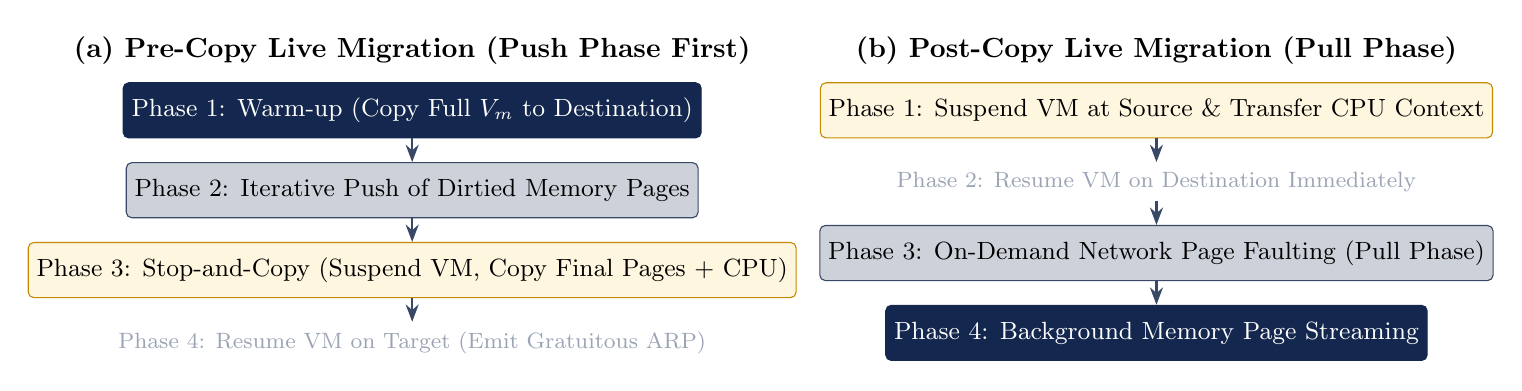
\begin{tikzpicture}[font=\footnotesize]
  % Pre-Copy Flow
  \node[dark, minimum width=6cm] (pre1) {Phase 1: Warm-up (Copy Full $V_m$ to Destination)};
  \node[mid, below=0.3cm of pre1, minimum width=6cm] (pre2) {Phase 2: Iterative Push of Dirtied Memory Pages};
  \node[gold, below=0.3cm of pre2, minimum width=6cm] (pre3) {Phase 3: Stop-and-Copy (Suspend VM, Copy Final Pages + CPU)};
  \node[steel, below=0.3cm of pre3, minimum width=6cm] (pre4) {Phase 4: Resume VM on Target (Emit Gratuitous ARP)};
  \draw[arr] (pre1) -- (pre2); \draw[arr] (pre2) -- (pre3); \draw[arr] (pre3) -- (pre4);
  \node[above=0.1cm of pre1, font=\bfseries] {(a) Pre-Copy Live Migration (Push Phase First)};

  % Post-Copy Flow
  \node[gold, right=1.5cm of pre1, minimum width=6cm] (post1) {Phase 1: Suspend VM at Source \& Transfer CPU Context};
  \node[steel, below=0.3cm of post1, minimum width=6cm] (post2) {Phase 2: Resume VM on Destination Immediately};
  \node[mid, below=0.3cm of post2, minimum width=6cm] (post3) {Phase 3: On-Demand Network Page Faulting (Pull Phase)};
  \node[dark, below=0.3cm of post3, minimum width=6cm] (post4) {Phase 4: Background Memory Page Streaming};
  \draw[arr] (post1) -- (post2); \draw[arr] (post2) -- (post3); \draw[arr] (post3) -- (post4);
  \node[above=0.1cm of post1, font=\bfseries] {(b) Post-Copy Live Migration (Pull Phase)};
\end{tikzpicture}
\caption{Algorithmic Comparison: Pre-Copy vs Post-Copy Live Migration.}
\end{figure}

\subsection{Pre-Copy Iterative Live Migration}
Employed by Xen, KVM, and VMware ESXi, Pre-Copy migration relies on a \textbf{Push} model:
\begin{enumerate}[leftmargin=*]
  \item \textbf{Pre-Copy Initialization:} The source VM continues executing normally while the hypervisor copies the entire memory space ($V_m$) to the target host.
  \item \textbf{Iterative Pre-Copying:} As the guest OS executes, it modifies memory pages (creating ``dirty pages''). The hypervisor uses shadow page tables or hardware dirty-bit tracking to log modified pages and re-transmits them in successive iterations.
  \item \textbf{Mathematical Convergence Criterion:}
    Let $D$ denote the memory dirtying rate (MB/s) and $R$ the network transmission rate (MB/s). The data remaining to be sent in iteration $k+1$ is:
    \begin{equation}
    V_{k+1} = V_k \times \left( \frac{D}{R} \right) = V_m \cdot r^{k+1}, \quad \text{where } r = \frac{D}{R}
    \end{equation}
    \begin{thmbox}{Pre-Copy Convergence Condition}
    The iterative series converges to zero if and only if the dirtying rate is strictly less than the network transmission rate:
    \begin{equation}
    r = \frac{D}{R} < 1 \iff D < R
    \end{equation}
    If the VM executes a write-intensive workload where $D \ge R$, memory is dirtied faster than the network can transmit it. The iterative process will \textbf{never converge}, dramatically increasing migration duration and network bandwidth consumption!
    \end{thmbox}
  \item \textbf{Stop-and-Copy Phase:} When remaining dirty pages drop below a threshold (or a maximum round limit is reached), the source VM is suspended. The remaining dirty pages and CPU execution state are transmitted.
  \item \textbf{Resume Phase:} The VM is resumed on the target host.
\end{enumerate}

\subsection{Post-Copy Live Migration}
Post-Copy reverses the sequence:
\begin{enumerate}[leftmargin=*]
  \item The VM is suspended immediately on the source host.
  \item Its minimal processor state ($\mathcal{C}_{\text{CPU}}$) is transferred to the destination.
  \item The VM is \textbf{resumed on the destination immediately}!
  \item When the VM accesses a memory page not yet present on the target, a network page fault traps execution, pulling the required page from the source host on demand (\textbf{Pull Phase}).
  \item Remaining pages are pushed in the background.
  \item \textbf{Key Advantage:} Every memory page is transmitted across the network \textbf{at most once}, guaranteeing that total data transferred equals exactly $V_m$, minimizing energy consumption and eliminating convergence failure.
\end{enumerate}

\section{Linux Kernel Container Primitives}
Modern container runtimes (Docker, containerd, CRI-O) do not use hypervisors; they construct isolated user-space sandboxes using two fundamental Linux kernel subsystems:

\begin{figure}[H]
\centering
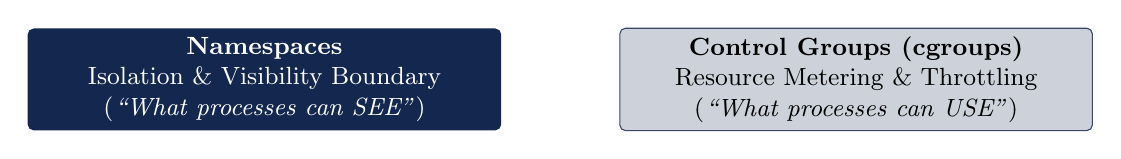
\begin{tikzpicture}[font=\small]
  \node[dark, minimum width=6cm, minimum height=1cm] (ns) {\textbf{Namespaces}\\Isolation \& Visibility Boundary\\(\emph{``What processes can SEE''})};
  \node[mid, right=1.5cm of ns, minimum width=6cm, minimum height=1cm] (cg) {\textbf{Control Groups (cgroups)}\\Resource Metering \& Throttling\\(\emph{``What processes can USE''})};
\end{tikzpicture}
\caption{The Two Pillars of Linux Container Virtualization.}
\end{figure}

\subsection{Linux Namespaces: Isolation of System Views}
Namespaces wrap global system resources in an abstraction that makes it appear to processes within the namespace that they possess their own isolated instance of the resource:
\begin{center}
\begin{tabularx}{\textwidth}{>{\bfseries}l l X}
\toprule
Namespace & Flag & Isolated System Resource\\
\midrule
PID & \texttt{CLONE\_NEWPID} & Process IDs. A container process sees itself as PID 1 (init), isolated from host PIDs.\\
NET & \texttt{CLONE\_NEWNET} & Network devices, IP routing tables, port bindings, firewall rules (iptables).\\
MNT & \texttt{CLONE\_NEWNS} & Filesystem mount points. Isolates container rootfs from the host root directory.\\
IPC & \texttt{CLONE\_NEWIPC} & System V Inter-Process Communication and POSIX message queues.\\
UTS & \texttt{CLONE\_NEWUTS} & Hostname and NIS domain name.\\
USER & \texttt{CLONE\_NEWUSER} & User and Group ID mappings. Allows root inside a container to map to an unprivileged user outside.\\
CGROUP & \texttt{CLONE\_NEWCGROUP} & Cgroup hierarchy visibility.\\
\bottomrule
\end{tabularx}
\end{center}

\subsection{Control Groups (cgroups): Resource Allocation and Quotas}
While namespaces prevent a container from seeing other processes, they do not restrict resource consumption. Without cgroups, a malicious container could execute an infinite loop or memory leak, starving the host. \textbf{Control Groups (cgroups)} meter, prioritize, and enforce hard limits on:
\begin{itemize}[leftmargin=*]
  \item \textbf{CPU Shares and Quotas (\texttt{cpu.cfs\_quota\_us}):} Enforcing strict CPU bandwidth allocations.
  \item \textbf{Memory Limits (\texttt{memory.limit\_in\_bytes}):} Enforcing hard memory ceilings; triggers Out-Of-Memory (OOM) killer if exceeded.
  \item \textbf{Block I/O (\texttt{blkio}):} Throttling disk read/write bandwidth and IOPS.
  \item \textbf{Device Access (\texttt{devices}):} Restricting access to physical character and block devices.
\end{itemize}

\subsection{Docker Storage Persistence: Named Volumes}
Docker container writable layers are ephemeral; deleting a container purges all files written to its top layer. To persist data (e.g., database files):
\begin{itemize}[leftmargin=*]
  \item \textbf{Docker Named Volumes:} Persistent storage directories managed by Docker located on the host filesystem (\texttt{/var/lib/docker/volumes/}).
  \item \textbf{Lifecycle Decoupling:} If a database container is stopped or deleted, data residing inside an attached Docker named volume \textbf{remains completely intact and unaffected}.
\end{itemize}

\section{Comprehensive Solved Assignment Problems (Week 10)}

\begin{solved}{Condition Increasing Live Migration Duration}
\Given During live VM migration, which condition is most likely to increase the total migration time?
\Steps
\begin{enumerate}[leftmargin=*]
  \item In pre-copy live migration, the hypervisor iteratively copies dirty pages.
  \item If the guest application modifies memory rapidly (\textbf{high rate of memory-page modification}, $D \ge R$), each iteration generates massive volumes of dirty pages, preventing rapid convergence and increasing total migration time.
\end{enumerate}
\Answer \textbf{High rate of memory-page modification by the VM}.
\end{solved}

\begin{solved}{Post-Copy Live Migration Mechanics}
\Given Which live VM migration technique starts the VM on the destination first and then fetches memory pages from the source on demand as they are accessed?
\Steps
\begin{enumerate}[leftmargin=*]
  \item \textbf{Post-Copy Migration} suspends the VM, transfers the execution context to resume on the target immediately, and pulls memory pages across the network on-demand when page faults occur.
\end{enumerate}
\Answer \textbf{Post-copy migration}.
\end{solved}

\begin{solved}{Minimizing Data and Energy in Pre-Copy Migration}
\Given Which technique is most likely to reduce the total data transferred and energy consumed during pre-copy live migration?
\Steps
\begin{enumerate}[leftmargin=*]
  \item Compressing memory pages before network transmission reduces the total number of bytes transferred over the link, saving network bandwidth and transceiver energy.
\end{enumerate}
\Answer \textbf{Compressing memory pages before transmission}.
\end{solved}

\begin{solved}{Resource Management to Prevent Fog Overload}
\Given What resource management strategy is most important to prevent overload when many edge devices send telemetry to nearby fog nodes?
\Steps
\begin{enumerate}[leftmargin=*]
  \item Implementing dynamic load balancing and cooperative workload shedding across neighboring fog nodes distributes load evenly and avoids localized saturation.
\end{enumerate}
\Answer \textbf{Dynamic load balancing and workload offloading among fog nodes}.
\end{solved}

\begin{solved}{Kubernetes Pod Placement Component}
\Given Which Kubernetes component assigns newly created Pods to appropriate worker nodes based on resource constraints?
\Steps
\begin{enumerate}[leftmargin=*]
  \item The \textbf{\texttt{kube-scheduler}} filters and scores candidate nodes based on CPU/RAM availability, taints, tolerations, and affinity rules to select the optimal host for each Pod.
\end{enumerate}
\Answer \textbf{\texttt{kube-scheduler}}.
\end{solved}

\begin{solved}{Docker Build Output Artifact}
\Given In the workflow: \texttt{Dockerfile $\to$ docker build $\to$ \_\_\_\_\_\_ $\to$ docker run}, which entity is produced?
\Steps
\begin{enumerate}[leftmargin=*]
  \item The \texttt{docker build} command compiles the declarative instructions of a Dockerfile into an immutable, multi-layered \textbf{Docker image}.
\end{enumerate}
\Answer \textbf{Docker image}.
\end{solved}

\begin{solved}{Roles of Linux Namespaces and cgroups}
\Given Which statement correctly describes the division of responsibilities between Linux namespaces and cgroups?
\Steps
\begin{enumerate}[leftmargin=*]
  \item \textbf{Namespaces} isolate system views (processes, networks, mounts).
  \item \textbf{Control groups (cgroups)} meter, prioritize, and limit hardware resource consumption (CPU, memory, disk I/O).
\end{enumerate}
\Answer \textbf{Namespaces provide isolation of processes and system resources, while cgroups regulate resource usage}.
\end{solved}

\begin{solved}{Cold Migration Duration Computation}
\Given Memory size $V_m = 32\text{ GB}$, usable network bandwidth $R = 16\text{ MB/s}$. Find approximate transfer duration.
\Steps
\begin{equation}
V_m = 32 \times 1024\text{ MB} = 32,768\text{ MB}
\end{equation}
\begin{equation}
T = \frac{32,768\text{ MB}}{16\text{ MB/s}} = 2048\text{ s} \approx 34.13\text{ minutes}
\end{equation}
\Answer \textbf{About 34 minutes}.
\end{solved}

\begin{solved}{Docker Named Volume Data Persistence}
\Given A database container is accidentally deleted, but its data files were stored in a Docker named volume. What happens to the data?
\Steps
\begin{enumerate}[leftmargin=*]
  \item Docker named volumes exist independently of container lifecycles on the host filesystem.
  \item Deleting the container has zero impact on the volume; the data remains completely intact and can be mounted to a new container.
\end{enumerate}
\Answer \textbf{The data persists safely within the named volume on the host}.
\end{solved}

\begin{solved}{Core Comparison Between Containers and VMs}
\Given Which statement about containers and virtual machines is correct?
\Steps
\begin{enumerate}[leftmargin=*]
  \item Virtual Machines virtualize physical hardware and execute separate guest OS kernels.
  \item Containers share the host operating system kernel and isolate applications at the process level.
\end{enumerate}
\Answer \textbf{Containers share the host operating system kernel, whereas virtual machines run separate guest operating systems}.
\end{solved}

% ==================================================================
%  WEEK 11
% ==================================================================
\chapter{Emerging Paradigms: Dew Computing, Serverless Architecture, and Sustainable Cloud}

\section{Introduction and Week Overview}
Week 11 investigates modern evolutionary paradigms that transcend traditional centralized server infrastructure. As distributed computing advances toward the extreme network edge and operational costs skyrocket, the curriculum addresses three cutting-edge domains:
\begin{enumerate}[leftmargin=*]
  \item \textbf{Dew Computing (DC):} Bringing cloud microservice capabilities directly to end devices to eliminate absolute internet dependency, balancing independence and cloud collaboration.
  \item \textbf{Serverless Computing and Function-as-a-Service (FaaS):} Fine-grained, event-driven execution abstractions that completely mask server administration, scale to zero, and bill strictly for resource runtime.
  \item \textbf{Sustainable and Green Cloud Computing:} Architectural frameworks, power-regulation strategies, and economic models designed to curb the escalating multi-terawatt energy consumption and carbon footprints of hyperscale Cloud Data Centers (CDCs).
\end{enumerate}

\section{Dew Computing Foundations}
\subsection{Motivation: Overcoming the Internet Dependency Bottleneck}
While Cloud Computing provides virtually infinite computation and storage, it exhibits a fundamental vulnerability: \textbf{mandatory continuous Internet connectivity}. If network access is severed due to infrastructure failure, remote geography, or catastrophic events, traditional cloud services become entirely inaccessible.

\begin{defbox}{Dew Computing (DC)}
\textbf{Dew Computing} is an information technology paradigm where on-premises personal computing devices (smartphones, PCs, edge gateways) host lightweight, autonomous microservices that operate independently of an active Internet connection while collaborating with the centralized cloud whenever network connectivity is available.
\end{defbox}

\begin{figure}[H]
\centering
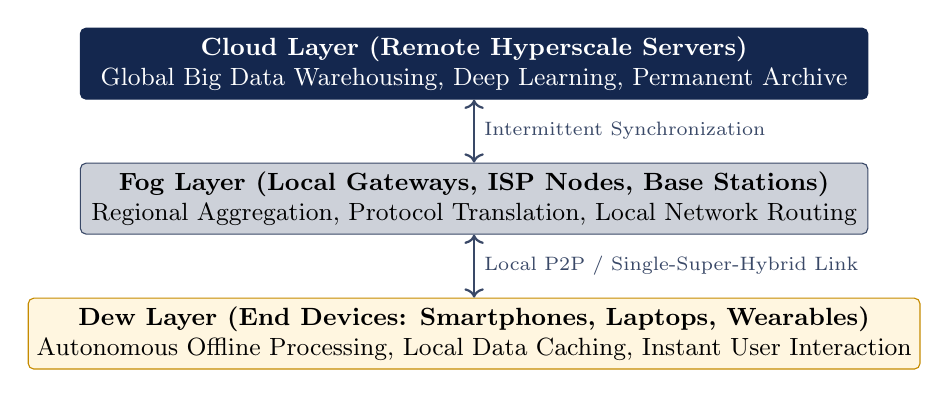
\begin{tikzpicture}[node distance=1.2cm, font=\small]
  \node[dark, minimum width=10cm, minimum height=0.9cm] (cloud) {\textbf{Cloud Layer (Remote Hyperscale Servers)}\\Global Big Data Warehousing, Deep Learning, Permanent Archive};
  \node[mid, below=0.8cm of cloud, minimum width=10cm, minimum height=0.9cm] (fog) {\textbf{Fog Layer (Local Gateways, ISP Nodes, Base Stations)}\\Regional Aggregation, Protocol Translation, Local Network Routing};
  \node[gold, below=0.8cm of fog, minimum width=10cm, minimum height=0.9cm] (dew) {\textbf{Dew Layer (End Devices: Smartphones, Laptops, Wearables)}\\Autonomous Offline Processing, Local Data Caching, Instant User Interaction};

  \draw[arr, <->] (cloud) -- node[right, font=\scriptsize] {Intermittent Synchronization} (fog);
  \draw[arr, <->] (fog) -- node[right, font=\scriptsize] {Local P2P / Single-Super-Hybrid Link} (dew);
\end{tikzpicture}
\caption{The Meteorological Hierarchy: Cloud (Sky) $\to$ Fog (Near Ground) $\to$ Dew (On the Ground).}
\end{figure}

\subsection{Core Principles: Independence and Collaboration}
Introduced by Yingwei Wang, the operational philosophy of Dew Computing rests upon two dual pillars:
\begin{itemize}[leftmargin=*]
  \item \textbf{Independence:} The local device must provide full or graceful core service functionality entirely offline without depending on continuous Internet or remote server availability.
  \item \textbf{Collaboration:} When network connectivity is established, local applications must automatically discover cloud endpoints, synchronize delta state modifications, and reconcile conflicts seamlessly.
\end{itemize}

A canonical everyday realization of Dew Computing is \textbf{Dropbox} or \textbf{Google Drive Desktop}: users read, edit, create, and delete files locally inside an offline directory without network access (independence). The moment an Internet connection is detected, background synchronization daemons propagate file deltas to the remote cloud server (collaboration).

\subsection{Dew Service Architecture Taxonomy}
Analogous to the classical SPI model of cloud computing, Dew Computing introduces a granular service taxonomy:
\begin{center}
\begin{tabularx}{\textwidth}{>{\bfseries}l X X}
\toprule
Dew Service Model & Definition & Exemplary Realization\\
\midrule
Software-In-Dew (SiD) & Software configuration, license ownership, and code metadata are mastered in the cloud, while local runtime binaries execute independently offline on the end device. & Local office productivity suites with cloud license sync; offline mobile apps.\\
\addlinespace
Platform-In-Dew (PiD) & Development runtime environments, APIs, and micro-frameworks exist on the local device, enabling local compilation and execution with cloud registry synchronization. & Local Docker container runtimes, offline Python/Node development toolchains.\\
\addlinespace
Infrastructure-As-Dew (IaD) & Hardware capabilities (CPU, RAM, local storage) of diverse end devices are virtualized and pooled into local ad-hoc processing clusters. & P2P distributed file storage across office PCs; local Bluetooth mesh processing.\\
\addlinespace
Database-In-Dew (DbID) & A lightweight local database engine (e.g., SQLite, Realm) processes queries locally with sub-millisecond response and synchronizes transactional deltas to cloud databases. & Mobile banking offline transaction caching; offline relational records.\\
\addlinespace
Website-In-Dew (WiD) & A complete local web server instance runs directly on the client machine, rendering pages locally from cached templates and syncing dynamic content on reconnect. & Progressive Web Apps (PWAs) with Service Workers caching dynamic offline assets.\\
\addlinespace
Storage-In-Dew (StID) & File data resides permanently in local non-volatile storage while background threads synchronize snapshots to remote cloud buckets. & Dropbox local file sync; OneDrive Smart Files offline mirrors.\\
\bottomrule
\end{tabularx}
\end{center}

\section{Serverless Computing and Function-as-a-Service (FaaS)}
\subsection{The Paradigm Shift from Servers to Applications}
In classical IaaS, developers rent virtual machines and must manage operating system patches, kernel configurations, firewall rules, and scaling thresholds. In PaaS, while OS management is abstracted, developers still configure server instances, manage runtime pools, and pay for idle compute capacity.

\textbf{Serverless Computing} elevates abstraction to the highest level: the cloud customer writes only modular, stateless business logic functions. The cloud provider assumes $100\%$ of operational responsibilities---including provisioning hardware, container lifecycle management, automated horizontal scaling, high availability, and fault tolerance.

\begin{figure}[H]
\centering
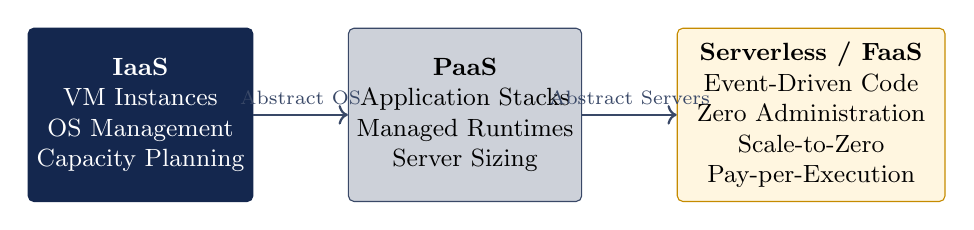
\begin{tikzpicture}[node distance=0.8cm, font=\small]
  \node[dark, minimum width=2.8cm, minimum height=2.2cm] (iaas) {\textbf{IaaS}\\VM Instances\\OS Management\\Capacity Planning};
  \node[mid, right=1.2cm of iaas, minimum width=2.8cm, minimum height=2.2cm] (paas) {\textbf{PaaS}\\Application Stacks\\Managed Runtimes\\Server Sizing};
  \node[gold, right=1.2cm of paas, minimum width=3.4cm, minimum height=2.2cm] (serverless) {\textbf{Serverless / FaaS}\\Event-Driven Code\\Zero Administration\\Scale-to-Zero\\Pay-per-Execution};

  \draw[arr, ->] (iaas) -- node[above, font=\scriptsize] {Abstract OS} (paas);
  \draw[arr, ->] (paas) -- node[above, font=\scriptsize] {Abstract Servers} (serverless);
\end{tikzpicture}
\caption{Evolutionary Trajectory of Cloud Abstraction Layers.}
\end{figure}

\subsection{Architectural Characteristics of FaaS}
\begin{itemize}[leftmargin=*]
  \item \textbf{Fine-Grained Granularity:} Applications are partitioned into discrete, single-purpose functions (e.g., resizing an image, validating an authentication token, parsing an incoming webhook).
  \item \textbf{Event-Driven Activation:} Functions execute strictly in response to designated asynchronous or synchronous triggers:
    \begin{itemize}
      \item HTTP REST requests via API Gateways.
      \item Object storage notifications (e.g., file uploaded to AWS S3 bucket).
      \item Message broker streams (e.g., Apache Kafka, AWS Kinesis, RabbitMQ).
      \item Cron-like scheduled timers.
    \end{itemize}
  \item \textbf{Stateless Execution:} Functions retain no persistent internal state across invocations. Any required session state must be committed to external storage (e.g., Amazon DynamoDB, Redis, S3).
  \item \textbf{Automatic Scale-to-Zero and Scale-to-Infinity:} If zero requests arrive, zero instances run, and the customer incurs \textbf{\$0.00 cost}. If 10,000 concurrent requests arrive simultaneously, the cloud platform automatically spins up 10,000 isolated execution environments in parallel.
\end{itemize}

\subsection{The Serverless Cold Start Challenge}
When an incoming event triggers a serverless function that has no pre-warmed idle container ready in memory:
\begin{enumerate}[leftmargin=*]
  \item The FaaS control plane selects a physical host.
  \item It downloads the container image or code package.
  \item It instantiates an isolated sandbox (using microVMs such as AWS Firecracker).
  \item It initializes the language runtime (JVM, Python, Node.js) and executes global initialization code.
\end{enumerate}
This sequence introduces a \textbf{Cold Start Latency} (ranging from $100\text{ ms}$ for Node/Python to $>2\text{ seconds}$ for Java/JVM). Subsequent invocations reuse the warm container, executing with minimal latency ($< 10\text{ ms}$) until the container is recycled after an idle timeout window (typically 5 to 15 minutes).

\subsection{Serverless Economic Billing Formulation}
Serverless billing abandons hourly instance leasing in favor of exact sub-second consumption metering:
\begin{equation}
\text{Total FaaS Cost} = N_{\text{req}} \times C_{\text{req}} + \sum_{i=1}^{N_{\text{req}}} \left( M_i \times T_i \right) \times C_{\text{GB-sec}}
\end{equation}
Where:
\begin{itemize}[leftmargin=*]
  \item $N_{\text{req}}$: Total number of function invocations.
  \item $C_{\text{req}}$: Cost per million invocations (standardly $\$0.20$ per $10^6$ calls).
  \item $M_i$: Memory allocated to the function (in GB, e.g., $512\text{ MB} = 0.5\text{ GB}$).
  \item $T_i$: Execution duration of invocation $i$ rounded to the nearest millisecond.
  \item $C_{\text{GB-sec}}$: Unit cost per Gigabyte-second (standardly $\approx \$0.0000166667 / \text{GB}\cdot\text{s}$).
\end{itemize}

\section{Sustainable and Green Cloud Computing}
\subsection{The Data Center Energy Dilemma}
Hyperscale Cloud Data Centers (CDCs) have become the most power-dense industrial facilities on earth. Driven by machine learning training, real-time video streaming, and global cloud workflows:
\begin{itemize}[leftmargin=*]
  \item Global data center electricity consumption exceeded $200\text{ TWh}$ in 2020 and is projected to reach \textbf{8,000 TeraWatt-hours (TWh) by 2030} (representing nearly $10\%$ to $15\%$ of global electrical generation).
  \item Substantial electricity is generated from fossil fuel grids, translating directly into millions of metric tons of atmospheric $\text{CO}_2$ emissions.
\end{itemize}

\subsection{Energy Breakdown Within a Cloud Data Center}
Empirical measurements across modern enterprise data centers reveal that electricity consumption is distributed across five primary subsystems:
\begin{center}
\begin{tabularx}{\textwidth}{>{\bfseries}l c X}
\toprule
Subsystem & Typical Energy \% & Primary Operational Drivers\\
\midrule
Processors (CPUs / GPUs) & $45\%$ & Active computation, transistor switching, leakage current.\\
Cooling & $20\%$ & Chilled water plants, air handlers, CRAH units, fan walls.\\
Main Memory (RAM) & $15\%$ & Continuous capacitive DRAM refresh cycles.\\
Storage Subsystems & $10\%$ & Mechanical HDD spindle spinning, SSD flash controllers.\\
Networking Equipment & $10\%$ & Spine-leaf switches, optical transceivers, routers.\\
\bottomrule
\end{tabularx}
\end{center}

\subsection{Energy Efficiency Metrics: PUE and DCiE}
To benchmark environmental performance, the Green Grid consortium defined standardized metrics:
\begin{equation}
\text{Power Usage Effectiveness (PUE)} = \frac{\text{Total Facility Energy Consumption}}{\text{IT Equipment Energy Consumption}} = \frac{P_{\text{IT}} + P_{\text{Cooling}} + P_{\text{Lighting}} + P_{\text{Losses}}}{P_{\text{IT}}}
\end{equation}
An ideal theoretical data center with zero cooling or power conversion overhead has $\text{PUE} = 1.0$. Historical enterprise facilities operated at $\text{PUE} \approx 2.0$, whereas state-of-the-art hyperscale facilities (Google, Microsoft) achieve $\text{PUE} \approx 1.10 - 1.15$ using advanced evaporative cooling, AI-controlled temperature set-points, and direct-to-chip liquid cooling.

The reciprocal metric is \textbf{Data Center Infrastructure Efficiency (DCiE)}:
\begin{equation}
\text{DCiE} = \frac{1}{\text{PUE}} = \frac{\text{IT Equipment Energy Consumption}}{\text{Total Facility Energy Consumption}} \times 100\%
\end{equation}
A $\text{PUE}$ of $1.25$ corresponds to $\text{DCiE} = 80\%$.

\subsection{Power Management and Conservation Approaches}
Following the conceptual framework by Rajkumar Buyya and Sukhpal Singh Gill:
\begin{itemize}[leftmargin=*]
  \item \textbf{Dynamic Voltage and Frequency Scaling (DVFS):} CMOS CPU dynamic power scales cubically with clock frequency ($P \propto V^2 f \approx f^3$). Throttling clock frequency during light loads yields substantial energy savings. \emph{Tradeoff:} Lower frequencies prolong execution times, risking SLA response time violations.
  \item \textbf{Dynamic VM Consolidation:} Migrating VMs from lightly loaded servers onto a compact set of physical blades and switching empty hosts into low-power ACPI sleep states (e.g., C6/S3 states consuming $<10\text{ W}$ instead of $150\text{ W}$ idle power).
  \item \textbf{Thermal-Aware Scheduling:} Directing computationally heavy workloads to server racks located in cooler physical aisles or during nighttime hours to decrease refrigeration workload.
  \item \textbf{Renewable Energy Microgrids:} Powering data centers directly with co-located solar arrays, wind farms, and battery energy storage systems (BESS).
\end{itemize}

\section{Comprehensive Solved NPTEL-Style Questions (Week 11)}

\begin{solved}{Dew Computing Core Tenets (NPTEL Assessment Problem)}
\Given What are the two foundational operational principles that define the Dew Computing paradigm, and how do they interact?
\Steps
\begin{enumerate}[leftmargin=*]
  \item \textbf{Independence:} The client application executes autonomously on local device hardware without requiring an active or continuous Internet connection.
  \item \textbf{Collaboration:} The application detects cloud connectivity and synchronizes data updates, configurations, and state modifications with centralized cloud servers.
\end{enumerate}
\Answer \textbf{Independence and Collaboration}.
\end{solved}

\begin{solved}{Dew Service Model Classification}
\Given A mobile banking app allows a field loan officer to record customer transactions in a local SQLite database in offline villages. When returning to the branch office, the app automatically syncs transactional records to the bank's central Oracle database in the cloud. Which Dew service model is exemplified?
\Steps
\begin{enumerate}[leftmargin=*]
  \item The core mechanism is a local structured database engine handling queries locally and synchronizing transactional deltas with a cloud database.
  \item By taxonomy definition, this matches Database-In-Dew (DbID).
\end{enumerate}
\Answer \textbf{Database-In-Dew (DbID)}.
\end{solved}

\begin{solved}{Serverless FaaS Economic Cost Calculation}
\Given A microservice deployed on AWS Lambda executes $10,000,000$ invocations in a month. Each invocation runs for an average duration of $200\text{ ms}$ and is configured with $512\text{ MB}$ ($0.5\text{ GB}$) of RAM. Given pricing:
\begin{itemize}
  \item Invocation charge: $\$0.20$ per $1,000,000$ requests.
  \item Compute charge: $\$0.0000166667$ per $\text{GB}\cdot\text{second}$.
\end{itemize}
Calculate the total monthly serverless execution cost.
\Steps
\begin{enumerate}[leftmargin=*]
  \item \textbf{Invocation Request Cost:}
  \begin{equation}
  \text{Cost}_{\text{req}} = \frac{10,000,000}{1,000,000} \times \$0.20 = 10 \times \$0.20 = \$2.00
  \end{equation}
  \item \textbf{Compute Duration in GB-Seconds:}
  \begin{equation}
  \text{Execution Time per Request} = 200\text{ ms} = 0.20\text{ seconds}
  \end{equation}
  \begin{equation}
  \text{GB-seconds per Request} = 0.5\text{ GB} \times 0.20\text{ s} = 0.10\text{ GB}\cdot\text{s}
  \end{equation}
  \begin{equation}
  \text{Total GB-seconds} = 10,000,000 \times 0.10\text{ GB}\cdot\text{s} = 1,000,000\text{ GB}\cdot\text{s}
  \end{equation}
  \item \textbf{Compute Charge:}
  \begin{equation}
  \text{Cost}_{\text{compute}} = 1,000,000 \times \$0.0000166667 = \$16.67
  \end{equation}
  \item \textbf{Total Monthly Settlement:}
  \begin{equation}
  \text{Total Cost} = \$2.00 + \$16.67 = \$18.67
  \end{equation}
\end{enumerate}
\Answer Total monthly serverless cost is \textbf{\$18.67}.
\end{solved}

\begin{solved}{Serverless Cold Start Optimization Mechanism}
\Given Which of the following strategies is most effective for mitigating cold-start latency in production FaaS architectures?
\Steps
\begin{enumerate}[leftmargin=*]
  \item Cold starts occur when the provider must instantiate a new runtime container sandbox from scratch.
  \item Provisioned Concurrency / Pre-warming keeps a predetermined number of initialized container sandboxes permanently resident in memory, eliminating runtime initialization delay for latency-critical traffic.
\end{enumerate}
\Answer \textbf{Provisioned Concurrency (Pre-warming container instances)}.
\end{solved}

\begin{solved}{Data Center PUE and DCiE Formulation}
\Given A cloud data center consumes a total of $25\text{ MegaWatts (MW)}$ of electrical power. Measurements indicate that internal IT equipment (servers, storage arrays, switches) consumes $16\text{ MW}$, while cooling, lighting, and power distribution account for the remaining $9\text{ MW}$. Find the Power Usage Effectiveness (PUE) and Data Center Infrastructure Efficiency (DCiE).
\Steps
\begin{enumerate}[leftmargin=*]
  \item \textbf{Compute PUE:}
  \begin{equation}
  \text{PUE} = \frac{\text{Total Power}}{\text{IT Power}} = \frac{25\text{ MW}}{16\text{ MW}} = 1.5625
  \end{equation}
  \item \textbf{Compute DCiE:}
  \begin{equation}
  \text{DCiE} = \frac{\text{IT Power}}{\text{Total Power}} \times 100\% = \frac{16}{25} \times 100\% = 64.0\%
  \end{equation}
  \begin{equation}
  \text{Verification: } \text{DCiE} = \frac{1}{\text{PUE}} = \frac{1}{1.5625} = 0.64 = 64\%
  \end{equation}
\end{enumerate}
\Answer \textbf{$\text{PUE} = 1.5625$}, \textbf{$\text{DCiE} = 64.0\%$}.
\end{solved}

\begin{solved}{Component Energy Distribution in Hyperscale Data Centers}
\Given According to empirical data center surveys highlighted in NPTEL Lecture 54, which subsystem consumes the single largest fraction of electrical energy inside a cloud data center?
\Steps
\begin{enumerate}[leftmargin=*]
  \item Empirical energy breakdown: Processors (CPUs/GPUs) account for $\approx 45\%$, Cooling for $\approx 20\%$, Memory for $\approx 15\%$, Storage for $\approx 10\%$, and Networking for $\approx 10\%$.
\end{enumerate}
\Answer \textbf{Processors (CPUs / GPUs) at approximately 45\% of total energy}.
\end{solved}

\begin{solved}{DVFS Power vs Latency Tradeoff}
\Given A server CPU operates at voltage $V = 1.2\text{ V}$ and frequency $f = 3.0\text{ GHz}$, drawing dynamic power $P_1 = 100\text{ W}$. If the hypervisor lowers the frequency to $f' = 2.0\text{ GHz}$ and reduces supply voltage to $V' = 1.0\text{ V}$, compute the new dynamic power dissipation $P_2$ assuming $P \propto V^2 f$.
\Steps
\begin{enumerate}[leftmargin=*]
  \item Using the CMOS power formula:
  \begin{equation}
  \frac{P_2}{P_1} = \frac{(V')^2 \cdot f'}{V^2 \cdot f} = \frac{(1.0)^2 \times 2.0}{(1.2)^2 \times 3.0} = \frac{1.0 \times 2.0}{1.44 \times 3.0} = \frac{2.0}{4.32} \approx 0.463
  \end{equation}
  \item New dynamic power:
  \begin{equation}
  P_2 = 100\text{ W} \times 0.463 = 46.3\text{ Watts}
  \end{equation}
  \item \textbf{Observation:} Energy dissipation drops by $53.7\%$, but task execution duration increases by $50\%$ ($\frac{3.0}{2.0} = 1.5$), which can violate tight SLA deadlines.
\end{enumerate}
\Answer New dynamic power is \textbf{46.3 Watts} ($53.7\%$ reduction).
\end{solved}

\begin{solved}{State Management in Serverless Function Architecture}
\Given Why are serverless functions strictly mandated to be stateless by cloud providers?
\Steps
\begin{enumerate}[leftmargin=*]
  \item Statelessness allows the provider to dynamically spawn, destroy, or route requests to any function instance across arbitrary physical nodes without synchronizing internal memory states.
  \item State persistence must be delegated to scalable shared external data stores (e.g., DynamoDB, Redis, S3).
\end{enumerate}
\Answer \textbf{To enable arbitrary horizontal scalability, rapid instantiation, and zero-downtime routing without cross-instance synchronization overhead}.
\end{solved}

\begin{solved}{Website-In-Dew (WiD) Operational Mechanism}
\Given In the Dew Computing framework, how does Website-In-Dew (WiD) serve web applications during complete network disconnection?
\Steps
\begin{enumerate}[leftmargin=*]
  \item WiD deploys a lightweight local web server or Progressive Web App Service Worker on the user's client machine.
  \item Static assets and dynamic data templates cached locally are rendered without querying the remote web server. Delta updates sync automatically upon reconnecting.
\end{enumerate}
\Answer \textbf{A local web service instance renders cached web content locally on the client machine, maintaining usability offline}.
\end{solved}

\begin{solved}{Dynamic VM Consolidation Energy Savings}
\Given A data center contains 200 servers. Each idle active server consumes $160\text{ W}$, while an active server running at $80\%$ load consumes $280\text{ W}$. A sleeping server in ACPI C6 state consumes $10\text{ W}$. Currently, 100 lightly loaded servers run at $20\%$ load (consuming $190\text{ W}$ each). By live migration, these workloads are consolidated onto 25 servers running at $80\%$ load, and the remaining 75 servers are placed into C6 sleep mode. Calculate the total power saved.
\Steps
\begin{enumerate}[leftmargin=*]
  \item \textbf{Initial Power Consumption:}
  \begin{equation}
  P_{\text{initial}} = 100 \times 190\text{ W} = 19,000\text{ Watts}
  \end{equation}
  \item \textbf{Post-Consolidation Power Consumption:}
  \begin{equation}
  P_{\text{active}} = 25 \times 280\text{ W} = 7,000\text{ Watts}
  \end{equation}
  \begin{equation}
  P_{\text{sleep}} = 75 \times 10\text{ W} = 750\text{ Watts}
  \end{equation}
  \begin{equation}
  P_{\text{final}} = 7,000 + 750 = 7,750\text{ Watts}
  \end{equation}
  \item \textbf{Net Power Savings:}
  \begin{equation}
  \Delta P = 19,000\text{ W} - 7,750\text{ W} = 11,250\text{ Watts} = 11.25\text{ kW}
  \end{equation}
  \begin{equation}
  \text{Percentage Reduction} = \frac{11,250}{19,000} \times 100\% = 59.21\%
  \end{equation}
\end{enumerate}
\Answer Total power saved is \textbf{11,250 Watts (11.25 kW)}, representing a \textbf{59.21\% reduction}.
\end{solved}

% ==================================================================
%  WEEK 12
% ==================================================================
\chapter{Advanced Paradigms and Case Studies: 5G Era, Cyber-Physical Systems, Spatial Cloud, and IoHT}

\section{Introduction and Week Overview}
Week 12 explores the confluence of cloud, edge, and modern telecommunication systems across complex real-world cyber-physical environments. The curriculum culminates with four interconnected pillars:
\begin{enumerate}[leftmargin=*]
  \item \textbf{Cloud Computing in the 5G Era:} How fifth-generation cellular networks, network softwarization, and multi-access edge computing (MEC) eliminate the communication latency bottleneck.
  \item \textbf{Cyber-Physical Systems (CPS) and Cloud Integration:} Bridging computational cyber cores with physical dynamics via closed-loop feedback, formalizing the NIST Cyber-Physical Cloud Computing (CPCC) architecture.
  \item \textbf{Case Study I --- Spatial Cloud Computing and Trajectory Cloud (Traj-Cloud):} Managing spatiotemporal big data, spatial indexing, distributed map-matching, and mobility trace mining over cloud infrastructure.
  \item \textbf{Case Study II --- Internet of Health Things (IoHT):} A complete four-tier hierarchical Cloud-Fog-Edge-IoT healthcare architecture evaluated empirically via iFogSim, physical embedded hardware prototypes, and Dew computing resilience.
\end{enumerate}

\section{Cloud Computing in the 5G Era}
\subsection{Generational Evolution of Mobile Networks}
Mobile telecommunications have evolved across distinct architectural epochs:
\begin{center}
\begin{tabularx}{\textwidth}{>{\bfseries}l l X l}
\toprule
Generation & Epoch & Core Capability \& Technology & Latency Benchmark\\
\midrule
1G & 1980s & Analog voice transmission (AMPS, TACS, NMT) & $\sim 1000\text{ ms}$\\
2G & Early 1990s & Digital voice, SMS, circuit-switched data (GSM, CDMA) & $\sim 300\text{--}500\text{ ms}$\\
3G & Early 2000s & Mobile packet data, early mobile web (UMTS, CDMA2000) & $\sim 100\text{--}150\text{ ms}$\\
4G LTE & 2010s & All-IP mobile broadband, video streaming, LTE-Advanced & $\sim 30\text{--}50\text{ ms}$\\
5G & 2020s+ & Multi-Gbps peak rates, ultra-low latency, massive IoT, MEC & $< 1\text{--}5\text{ ms}$\\
\bottomrule
\end{tabularx}
\end{center}

\subsection{The Three Functional Pillars of 5G}
The International Telecommunication Union (ITU-R) under IMT-2020 standardizes 5G capabilities across three distinct service categories:
\begin{figure}[H]
\centering
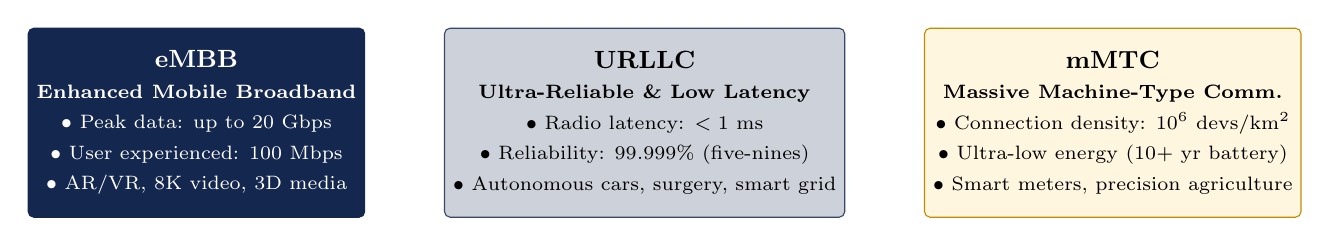
\begin{tikzpicture}[node distance=1.2cm, font=\small]
  \node[dark, minimum width=4.2cm, minimum height=2.4cm, align=center] (embb) {
    \textbf{eMBB}\\
    \scriptsize \textbf{Enhanced Mobile Broadband}\\
    \scriptsize $\bullet$ Peak data: up to $20\text{ Gbps}$\\
    \scriptsize $\bullet$ User experienced: $100\text{ Mbps}$\\
    \scriptsize $\bullet$ AR/VR, 8K video, 3D media
  };
  \node[mid, right=1.0cm of embb, minimum width=4.2cm, minimum height=2.4cm, align=center] (urllc) {
    \textbf{URLLC}\\
    \scriptsize \textbf{Ultra-Reliable \& Low Latency}\\
    \scriptsize $\bullet$ Radio latency: $< 1\text{ ms}$\\
    \scriptsize $\bullet$ Reliability: $99.999\%$ (five-nines)\\
    \scriptsize $\bullet$ Autonomous cars, surgery, smart grid
  };
  \node[gold, right=1.0cm of urllc, minimum width=4.2cm, minimum height=2.4cm, align=center] (mmtc) {
    \textbf{mMTC}\\
    \scriptsize \textbf{Massive Machine-Type Comm.}\\
    \scriptsize $\bullet$ Connection density: $10^6\text{ devs/km}^2$\\
    \scriptsize $\bullet$ Ultra-low energy ($10\text{+ yr battery}$)\\
    \scriptsize $\bullet$ Smart meters, precision agriculture
  };
\end{tikzpicture}
\caption{The ITU IMT-2020 5G Service Triangle.}
\end{figure}

\subsection{5G and Cloud Synergy: Softwarization and Edge Convergence}
The symbiosis between 5G and Cloud Computing operates in two directions:
\begin{enumerate}[leftmargin=*]
  \item \textbf{Cloudification of 5G (Network Softwarization):} 5G replaces proprietary telecommunication hardware with software running on commodity cloud data center servers via:
    \begin{itemize}
      \item \textbf{Software-Defined Networking (SDN):} Decoupling the network control plane (centralized decision-making) from the data forwarding plane.
      \item \textbf{Network Functions Virtualization (NFV):} Packaging firewalls, routers, EPC (Evolved Packet Core), and Baseband Units (BBUs) as virtualized network functions (VNFs) running on hypervisors or Kubernetes clusters.
      \item \textbf{Network Slicing:} Creating multiple isolated virtual networks on a single shared physical infrastructure, each customized to meet specific QoS guarantees (e.g., an eMBB slice for video streaming alongside a URLLC slice for robotic surgery).
    \end{itemize}
  \item \textbf{Cloud Evolution Driven by 5G (Multi-Access Edge Computing --- MEC):} Standardized by ETSI, MEC deploys cloud compute and storage resources directly at cellular Radio Access Network (RAN) base stations (gNodeB). By executing computation one hop away from User Equipment (UE), round-trip propagation delays drop from $50\text{--}100\text{ ms}$ (remote cloud) to under $5\text{ ms}$ (edge).
\end{enumerate}

\subsection{Mobile Cloud Computing (MCC) vs. MEC}
\begin{center}
\begin{tabularx}{\textwidth}{>{\bfseries}l X X}
\toprule
Dimension & Mobile Cloud Computing (MCC) & Multi-Access Edge Computing (MEC)\\
\midrule
Server Location & Centralized hyperscale cloud data centers across the wide-area Internet. & At local cellular base stations (gNodeB), aggregation points, or ISP gateways.\\
Latency & Moderate to high ($50\text{--}150\text{ ms}$) due to multi-hop WAN routing. & Ultra-low ($< 5\text{ ms}$) via direct one-hop wireless access.\\
Context Awareness & Low; cloud has no direct insight into real-time radio signal or user cell location. & High; access to real-time radio channel quality, cell congestion, and user velocity.\\
Bandwidth Pressure & Strains backhaul and core telecommunication networks. & Keeps high-volume traffic local, drastically reducing core network backhaul usage.\\
\bottomrule
\end{tabularx}
\end{center}

\section{Cyber-Physical Systems (CPS) and Cloud Integration}
\subsection{Foundations of Cyber-Physical Systems}
\begin{defbox}{Cyber-Physical System (CPS)}
Coined in 2006 by Helen Gill at the National Science Foundation (NSF), a \textbf{Cyber-Physical System (CPS)} is an orchestration of computational algorithms and physical components. Embedded computers monitor and control physical processes via feedback loops, where physical processes affect computational logic and vice versa.
\end{defbox}

CPS is characterized by the \textbf{intersection}, rather than the union, of the cyber world and the physical world:
\begin{equation}
\text{CPS} = \text{Cyber} \cap \text{Physical} = \{\text{Computation}\} \times \{\text{Dynamics}\} \times \{\text{Communication}\} \times \{\text{Control}\}
\end{equation}

\begin{figure}[H]
\centering
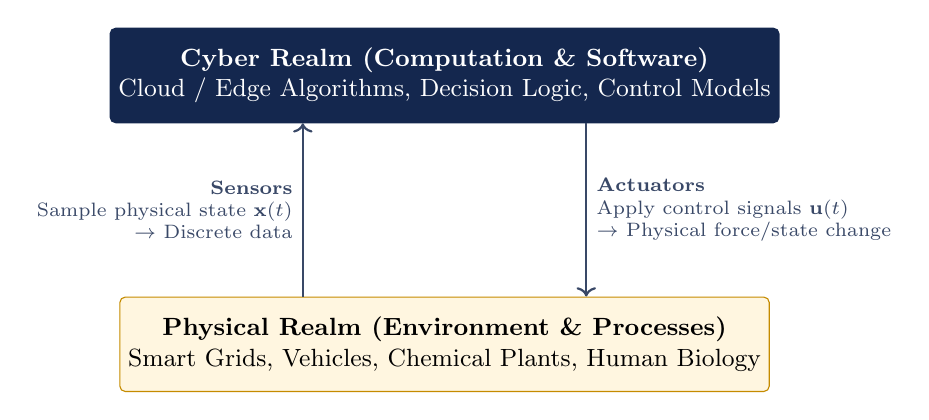
\begin{tikzpicture}[node distance=1.6cm, font=\small]
  \node[dark, minimum width=6cm, minimum height=1.2cm, align=center] (cyber) {\textbf{Cyber Realm (Computation \& Software)}\\Cloud / Edge Algorithms, Decision Logic, Control Models};
  \node[gold, below=2.2cm of cyber, minimum width=6cm, minimum height=1.2cm, align=center] (physical) {\textbf{Physical Realm (Environment \& Processes)}\\Smart Grids, Vehicles, Chemical Plants, Human Biology};

  \draw[arr, ->] ([xshift=-1.8cm]physical.north) -- node[left, font=\scriptsize, align=right] {\textbf{Sensors}\\Sample physical state $\mathbf{x}(t)$\\$\to$ Discrete data} ([xshift=-1.8cm]cyber.south);
  \draw[arr, ->] ([xshift=1.8cm]cyber.south) -- node[right, font=\scriptsize, align=left] {\textbf{Actuators}\\Apply control signals $\mathbf{u}(t)$\\$\to$ Physical force/state change} ([xshift=1.8cm]physical.north);
\end{tikzpicture}
\caption{Closed-Loop Feedback Architecture in Cyber-Physical Systems.}
\end{figure}

\subsection{CPS vs. Traditional Embedded Systems and IoT}
\begin{itemize}[leftmargin=*]
  \item \textbf{Embedded Systems:} Focus on standalone computation embedded within a host device (e.g., microwave microcontroller), rarely networked or aware of broad physical dynamics.
  \item \textbf{Internet of Things (IoT):} Focuses on uniquely identifiable objects connected to the Internet primarily for data aggregation, monitoring, and telemetry collection.
  \item \textbf{Cyber-Physical Systems (CPS):} Mandates tight, continuous, closed-loop bidirectional feedback control with hard temporal deadlines, stability guarantees, and safety-critical constraints.
\end{itemize}

\subsection{Cyber-Physical Cloud Computing (CPCC)}
In August 2013, the National Institute of Standards and Technology (NIST) published a landmark report establishing the \textbf{Cyber-Physical Cloud Computing (CPCC)} architectural framework:
\begin{defbox}{NIST CPCC Definition}
\textbf{Cyber-Physical Cloud Computing (CPCC)} is a system environment that can rapidly build, modify, and provision cyber-physical systems composed of a set of cloud computing-based sensor, processing, control, and data services.
\end{defbox}

\subsubsection{Key Benefits of CPCC}
\begin{enumerate}[leftmargin=*]
  \item \textbf{Resource Pooling and Scalability:} Dynamically aggregates heterogeneous sensor and actuator fleets across geographical boundaries.
  \item \textbf{Modular Composition:} Engineers can compose complex cyber-physical applications using modular microservices (Sensing-as-a-Service, Actuation-as-a-Service, Control-as-a-Service).
  \item \textbf{Cross-Domain Interoperability:} Translates disparate industrial and proprietary physical fieldbus protocols (Modbus, CAN bus, OPC-UA) into unified cloud APIs.
  \item \textbf{Adaptive Scaled Analytics:} Executes heavy predictive simulations (digital twins, finite element analysis) in the cloud while dispatching real-time control directives to the edge.
\end{enumerate}

\section{Case Study I: Spatial Cloud Computing and Traj-Cloud}
\subsection{Geospatial Data Characteristics}
Spatial (or geospatial) data describes objects, phenomena, or events located on or near the Earth's surface. Every spatial datum is formally modeled as a three-dimensional tuple:
\begin{equation}
\mathcal{D}_{\text{spatial}} = \langle \mathbf{L}, \mathbf{A}, \mathbf{T} \rangle
\end{equation}
where:
\begin{itemize}[leftmargin=*]
  \item $\mathbf{L} = (\text{Latitude}, \text{Longitude}, \text{Altitude})$ represents the geographical coordinate geometry.
  \item $\mathbf{A} = \{a_1, a_2, \dots, a_k\}$ represents non-spatial thematic attributes (e.g., road speed limit, patient ID, air pollution level).
  \item $\mathbf{T} = [t_{\text{start}}, t_{\text{end}}]$ represents the temporal validity lifespan.
\end{itemize}

\subsection{Spatial Cloud Computing Principles}
\begin{defbox}{Spatial Cloud Computing}
Spatial Cloud Computing is the cloud computing paradigm driven by geospatial sciences and optimized by spatiotemporal principles for enabling geospatial scientific discoveries within a distributed computing environment.
\end{defbox}

Key spatiotemporal principles leveraged to optimize cloud resources include:
\begin{itemize}[leftmargin=*]
  \item \textbf{Tobler's First Law of Geography:} ``Everything is related to everything else, but near things are more related than distant things.'' Cloud data partitioning strategies cluster spatially proximate points onto the same physical server nodes to minimize inter-node network shuffles.
  \item \textbf{Spatial Indexing (Quadtrees and R-Trees):} Standard B-trees fail in multi-dimensional space. Spatial cloud databases utilize R-trees (bounding box hierarchies) or Geohash-based spatial keys to achieve $\mathcal{O}(\log N)$ range and nearest-neighbor query performance.
\end{itemize}

\subsection{Traj-Cloud: Trajectory Cloud for Mobility Trace Mining}
Developed by researchers at IIT Kharagpur (S. Ghosh and S. K. Ghosh, IEEE COMSNETS 2019), \textbf{Traj-Cloud} is an end-to-end cloud platform designed to analyze massive GPS mobility trajectories for intelligent transportation systems (ITS) and smart-city applications.

\begin{figure}[H]
\centering
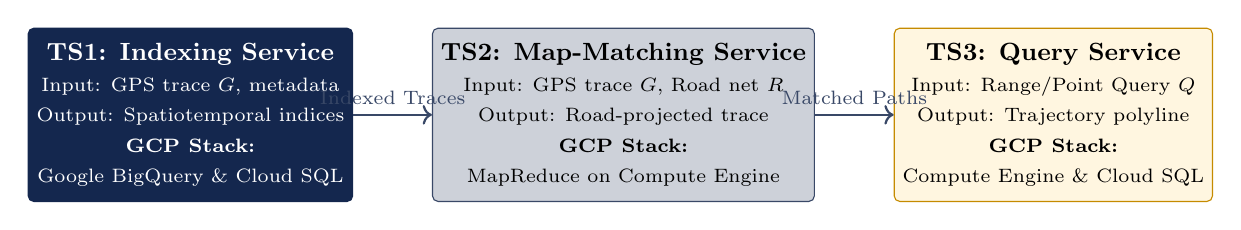
\begin{tikzpicture}[node distance=1.2cm, font=\small]
  \node[dark, minimum width=3.8cm, minimum height=2.2cm, align=center] (ts1) {
    \textbf{TS1: Indexing Service}\\
    \scriptsize Input: GPS trace $G$, metadata\\
    \scriptsize Output: Spatiotemporal indices\\
    \scriptsize \textbf{GCP Stack:}\\
    \scriptsize Google BigQuery \& Cloud SQL
  };
  \node[mid, right=1.0cm of ts1, minimum width=3.8cm, minimum height=2.2cm, align=center] (ts2) {
    \textbf{TS2: Map-Matching Service}\\
    \scriptsize Input: GPS trace $G$, Road net $R$\\
    \scriptsize Output: Road-projected trace\\
    \scriptsize \textbf{GCP Stack:}\\
    \scriptsize MapReduce on Compute Engine
  };
  \node[gold, right=1.0cm of ts2, minimum width=3.8cm, minimum height=2.2cm, align=center] (ts3) {
    \textbf{TS3: Query Service}\\
    \scriptsize Input: Range/Point Query $Q$\\
    \scriptsize Output: Trajectory polyline\\
    \scriptsize \textbf{GCP Stack:}\\
    \scriptsize Compute Engine \& Cloud SQL
  };

  \draw[arr, ->] (ts1) -- node[above, font=\scriptsize] {Indexed Traces} (ts2);
  \draw[arr, ->] (ts2) -- node[above, font=\scriptsize] {Matched Paths} (ts3);
\end{tikzpicture}
\caption{The Three Core Microservices of Traj-Cloud.}
\end{figure}

\begin{enumerate}[leftmargin=*]
  \item \textbf{TS1 --- Trajectory Data Indexing Service:} Takes raw, noisy GPS coordinates, assigns spatiotemporal bounding boxes, and ingests them into analytical distributed column stores (Google BigQuery) and transactional indexes (Cloud SQL).
  \item \textbf{TS2 --- Trajectory Map-Matching Service:} Raw GPS signals exhibit sampling drift and urban canyon interference. TS2 projects raw coordinates onto the true topological road network graph $R$ using distributed MapReduce algorithms on Google Compute Engine clusters to resolve ambiguities in near real-time.
  \item \textbf{TS3 --- Trajectory Query Service:} Executes high-throughput spatio-temporal range queries (``find all vehicles within 500 meters of junction $J$ between 09:00 and 09:15'') and trajectory similarity joins using Compute Engine worker pools.
\end{enumerate}

\section{Case Study II: Internet of Health Things (IoHT)}
\subsection{The Healthcare Paradigm Problem}
Continuous patient health monitoring (e.g., cardiac arrhythmia, epileptic seizures, post-operative vitals) generates massive high-velocity data streams from body-worn sensors. Transmitting continuous raw biometric streams directly to distant cloud data centers introduces fatal latency, consumes prohibitive cellular bandwidth, and suffers from total failure when Internet connectivity drops.

\subsection{The Four-Tier Hierarchical Network Topology}
To solve this, researchers at IIT Kharagpur designed a four-tier architecture:
\begin{figure}[H]
\centering
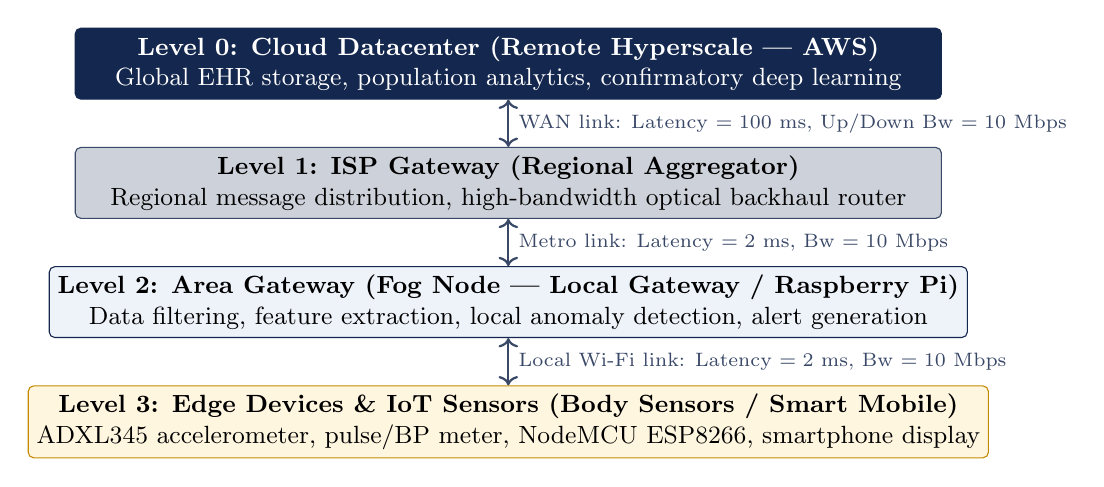
\begin{tikzpicture}[node distance=1.1cm, font=\small]
  \node[dark, minimum width=11cm, minimum height=0.9cm] (c0) {\textbf{Level 0: Cloud Datacenter (Remote Hyperscale --- AWS)}\\Global EHR storage, population analytics, confirmatory deep learning};
  \node[mid, below=0.6cm of c0, minimum width=11cm, minimum height=0.9cm] (f1) {\textbf{Level 1: ISP Gateway (Regional Aggregator)}\\Regional message distribution, high-bandwidth optical backhaul router};
  \node[box, below=0.6cm of f1, minimum width=11cm, minimum height=0.9cm] (f2) {\textbf{Level 2: Area Gateway (Fog Node --- Local Gateway / Raspberry Pi)}\\Data filtering, feature extraction, local anomaly detection, alert generation};
  \node[gold, below=0.6cm of f2, minimum width=11cm, minimum height=0.9cm] (e3) {\textbf{Level 3: Edge Devices \& IoT Sensors (Body Sensors / Smart Mobile)}\\ADXL345 accelerometer, pulse/BP meter, NodeMCU ESP8266, smartphone display};

  \draw[arr, <->] (c0) -- node[right, font=\scriptsize] {WAN link: Latency $= 100\text{ ms}$, Up/Down Bw $= 10\text{ Mbps}$} (f1);
  \draw[arr, <->] (f1) -- node[right, font=\scriptsize] {Metro link: Latency $= 2\text{ ms}$, Bw $= 10\text{ Mbps}$} (f2);
  \draw[arr, <->] (f2) -- node[right, font=\scriptsize] {Local Wi-Fi link: Latency $= 2\text{ ms}$, Bw $= 10\text{ Mbps}$} (e3);
\end{tikzpicture}
\caption{The 4-Tier Hierarchical Network Model for IoHT.}
\end{figure}

\subsection{Empirical Simulation Parameters (iFogSim Model)}
Based on the foundational iFogSim experiments presented in Lectures 59--60:
\begin{center}
\begin{tabularx}{\textwidth}{l r r r r r r}
\toprule
\textbf{Device Tier} & \textbf{MIPS} & \textbf{RAM (MB)} & \textbf{Up Bw (kbps)} & \textbf{Down Bw (kbps)} & \textbf{Level} & \textbf{Cost / MIPS}\\
\midrule
Cloud & $44,800$ & $40,000$ & $100$ & $10,000$ & $0$ & $\$0.01$\\
ISP Gateway & $2,800$ & $4,000$ & $10,000$ & $10,000$ & $1$ & $\$0.00$ (Local)\\
Area Gateway & $2,800$ & $4,000$ & $10,000$ & $10,000$ & $2$ & $\$0.00$ (Local)\\
Mobile Edge & $350$ & $1,000$ & $10,000$ & $270$ & $3$ & $\$0.00$ (User)\\
\bottomrule
\end{tabularx}
\end{center}

\subsubsection{Link Latency Distribution}
\begin{itemize}[leftmargin=*]
  \item Body Sensor $\to$ Mobile Edge: $1\text{ ms}$
  \item Mobile Edge $\to$ Area Gateway (Fog): $2\text{ ms}$
  \item Area Gateway $\to$ ISP Gateway: $2\text{ ms}$
  \item ISP Gateway $\to$ Cloud Datacenter: $100\text{ ms}$
  \item Mobile Edge $\to$ Local Display: $1\text{ ms}$
\end{itemize}

\subsection{Application Module Placement: Fog Model vs. Cloud Model}
The healthcare monitoring application consists of five logical modules:
\begin{center}
\begin{tabularx}{\textwidth}{>{\bfseries}l X X}
\toprule
Application Module & Placement in Fog-Based Model & Placement in Cloud-Based Model\\
\midrule
Client Module & Mobile Device (Edge, Level 3) & Mobile Device (Edge, Level 3)\\
Data Filtering Module & Area Gateway (Fog, Level 2) & Cloud Datacenter (Level 0)\\
Data Processing Module & Area Gateway (Fog, Level 2) & Cloud Datacenter (Level 0)\\
Event Handler Module & Area Gateway (Fog, Level 2) & Cloud Datacenter (Level 0)\\
Confirmatory Module & Cloud Datacenter (Level 0) & Cloud Datacenter (Level 0)\\
\bottomrule
\end{tabularx}
\end{center}

\subsection{Comparative Performance Evaluation Metrics}
Simulations across expanding configurations (Config 1: 4 users, Config 2: 8 users, Config 3: 16 users, Config 4: 32 users, Config 5: 64 users) revealed definitive findings:
\begin{enumerate}[leftmargin=*]
  \item \textbf{Control Loop Latency:} In the Fog model, because the control loop (Sensor $\to$ Mobile $\to$ Area Gateway $\to$ Event Handler $\to$ Display) executes entirely within Levels 2 and 3, latency remains virtually \textbf{constant and minimal} ($\approx 5\text{--}8\text{ ms}$), independent of user scale. In the Cloud model, every packet travels to Level 0 and back, causing latency exceeding $210\text{ ms}$, with severe queueing degradation as user count climbs.
  \item \textbf{Network Bandwidth Usage:} In the Fog model, only the few positive anomaly events trigger the Confirmatory Module on the cloud, resulting in negligible WAN traffic. In the Cloud model, continuous raw biometric telemetry is pumped to the cloud, congesting wide-area links.
  \item \textbf{Cost of Execution:} Fog devices (Area Gateways, Raspberry Pis) are customer-owned capital equipment incur zero per-second cloud billing fees. The Cloud model bills continuously for millions of MIPS, multiplying total operational cost.
  \item \textbf{Energy Consumption:} Mobile device energy remains identical across both architectures because the mobile edge performs the same sensor acquisition load. However, cloud data center energy drops by orders of magnitude under the Fog model.
\end{enumerate}

\subsection{Hardware Prototype Implementation}
The simulated IoHT architecture was physically built and validated using:
\begin{itemize}[leftmargin=*]
  \item \textbf{Biometric Sensor Node:} Customized Blood Pressure (BP) and Pulse meter outputting ASCII serial data at $9600\text{ baud}$.
  \item \textbf{Movement Tracking Sensor:} ADXL345 3-axis digital accelerometer sampling acceleration at high frequency.
  \item \textbf{Edge Acquisition Node:} NodeMCU ESP8266 board (CP2102) with integrated Wi-Fi microcontroller.
  \item \textbf{Fog Gateway Node:} Raspberry Pi 3 (64-bit ARM quad-core, $1\text{ GB}$ RAM, on-board Wi-Fi and Bluetooth).
  \item \textbf{Cloud Tier:} Amazon Web Services (AWS) EC2 instances.
\end{itemize}

\subsubsection{Signal Processing and Machine Learning Pipeline}
\begin{figure}[H]
\centering
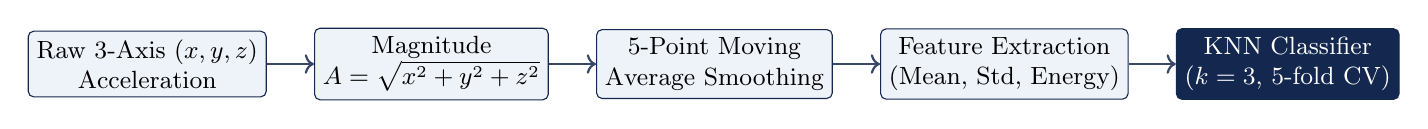
\begin{tikzpicture}[node distance=1.0cm, font=\small]
  \node[box] (raw) {Raw 3-Axis $(x,y,z)$\\Acceleration};
  \node[box, right=0.6cm of raw] (mag) {Magnitude\\$A = \sqrt{x^2+y^2+z^2}$};
  \node[box, right=0.6cm of mag] (smooth) {5-Point Moving\\Average Smoothing};
  \node[box, right=0.6cm of smooth] (feat) {Feature Extraction\\(Mean, Std, Energy)};
  \node[dark, right=0.6cm of feat] (knn) {KNN Classifier\\($k=3$, 5-fold CV)};

  \draw[arr, ->] (raw) -- (mag);
  \draw[arr, ->] (mag) -- (smooth);
  \draw[arr, ->] (smooth) -- (feat);
  \draw[arr, ->] (feat) -- (knn);
\end{tikzpicture}
\caption{Wearable Activity Classification Pipeline.}
\end{figure}

\begin{enumerate}[leftmargin=*]
  \item \textbf{Composite Magnitude Calculation:}
  \begin{equation}
  A[t] = \sqrt{x[t]^2 + y[t]^2 + z[t]^2}
  \end{equation}
  \item \textbf{5-Point Moving Average Smoothing:} To eliminate transient electronic noise, each sampled signal point is replaced by the mean of itself, its two predecessors, and its two successors:
  \begin{equation}
  \bar{A}[t] = \frac{A[t-2] + A[t-1] + A[t] + A[t+1] + A[t+2]}{5}
  \end{equation}
  \item \textbf{Feature Extraction:} Over sliding windows, six statistical features are extracted: Maximum Amplitude, Minimum Amplitude, Mean Amplitude, Standard Deviation in Amplitude, Energy in Time Domain ($\sum A[t]^2$), and Energy in Frequency Domain.
  \item \textbf{Classification via $k$-Nearest Neighbors (KNN):} Features are normalized via min-max scaling ($Y = \frac{x - \min}{\max - \min}$). Optimal parameter $k=3$ was established via 5-fold cross validation.
\end{enumerate}

\subsubsection{Demonstration Cardiac Risk Alert Logic}
The edge node calculates calibrated risk indicators:
\begin{equation}
f = (\text{KNN Activity Class Value}) + 1
\end{equation}
\begin{equation}
p = \frac{\text{BPM}}{f}, \quad s = \frac{\text{Systolic BP}}{f}, \quad d = \frac{\text{Diastolic BP}}{f}
\end{equation}
A severe emergency alarm triggers if:
\begin{equation}
(p \ge 170) \land (s \ge 180\text{ mmHg}) \land (d \ge 120\text{ mmHg}) \implies \text{HeartAttackAlarm} = \mathbf{True}
\end{equation}

\subsection{Dew Resilience Extension in Healthcare}
To prevent catastrophic patient monitoring blackouts when local fog routers or Internet backhauls fail:
\begin{itemize}[leftmargin=*]
  \item The smartphone or wearable edge node contains a \textbf{Dew Health Service Engine}.
  \item If Cloud or Fog connectivity is severed, the Dew engine immediately transitions to autonomous offline processing: vital signs are evaluated locally against emergency thresholds, acoustic patient alarms sound directly from the mobile handset, and time-stamped delta logs are stored in a local SQLite database (Database-in-Dew).
  \item The instant connectivity is restored, the Dew daemon reconciles and synchronizes all cached patient logs to the hospital cloud database.
\end{itemize}

\begin{center}
\begin{tabularx}{\textwidth}{>{\bfseries}l X X X}
\toprule
Metric & Pure Cloud & Cloud-Fog-Edge & With Dew Computing\\
\midrule
On-Premise Resource Utilization & Low & Sub-optimal & Optimal\\
Required Network Connectivity & Continuous Internet & Local Area Network & Fully Autonomous (Offline)\\
System Availability / Uptime & Low (Internet fragile) & High & Maximum (Fault-tolerant)\\
Bandwidth Demand & High (All data upstream) & Low (Alerts only) & Minimal (Delta sync)\\
Control Loop Latency & High ($> 200\text{ ms}$) & Ultra-low ($< 10\text{ ms}$) & Immediate ($< 2\text{ ms}$)\\
\bottomrule
\end{tabularx}
\end{center}

\newpage
\section{Comprehensive Solved NPTEL-Style Questions}

\begin{solved}{5G Service Pillar Categorization and QoS Matching}
\Given Categorize the following real-world applications into their primary 5G service pillar (\textbf{eMBB}, \textbf{URLLC}, or \textbf{mMTC}):
\begin{enumerate}[label=(\alph*),leftmargin=*]
  \item Autonomous vehicular collision avoidance system requiring $< 1\text{ ms}$ air interface latency.
  \item Streaming ultra-high-definition $8\text{K}$ $360^\circ$ virtual reality video to concert attendees.
  \item Smart agricultural soil moisture monitoring deploying 50,000 battery-powered sensors across farmland.
  \item Remote telesurgery robot operated by a specialist in a metropolitan hospital.
\end{enumerate}
\Steps
\begin{enumerate}[leftmargin=*]
  \item \textbf{Autonomous collision avoidance:} Demands sub-millisecond deterministic latency and $99.999\%$ transmission reliability to avert physical collisions $\implies$ \textbf{URLLC}.
  \item \textbf{$8\text{K}$ $360^\circ$ VR streaming:} Requires sustained multi-hundred Mbps throughput and wide radio channels, prioritizing high bandwidth over sub-millisecond delivery $\implies$ \textbf{eMBB}.
  \item \textbf{Smart agricultural soil sensors:} Exhibits extreme connection density, very low individual data rates, and multi-year battery lifespans without human maintenance $\implies$ \textbf{mMTC}.
  \item \textbf{Remote telesurgery robot:} Human tactile feedback and surgical tool precision require deterministic low latency ($< 5\text{ ms}$) and absolute reliability $\implies$ \textbf{URLLC}.
\end{enumerate}
\Answer (a) \textbf{URLLC}, (b) \textbf{eMBB}, (c) \textbf{mMTC}, (d) \textbf{URLLC}.
\end{solved}

\begin{solved}{MEC vs. Cloud Round-Trip Latency and Bandwidth Conservation}
\Given A connected vehicle captures high-definition camera frames generating a data payload of $S = 2\text{ MB}$ per event. The vehicle can offload image processing either to a local Multi-Access Edge Computing (MEC) server co-located at the base station or to a centralized Cloud data center:
\begin{itemize}[leftmargin=*]
  \item Uplink wireless radio bandwidth $R_{\text{radio}} = 100\text{ Mbps}$, one-hop radio latency $T_{\text{radio}} = 2\text{ ms}$.
  \item Core network backhaul bandwidth to Cloud $R_{\text{cloud}} = 20\text{ Mbps}$, wide-area propagation delay $T_{\text{wan}} = 45\text{ ms}$.
  \item Processing execution duration on MEC server: $T_{\text{proc, MEC}} = 30\text{ ms}$.
  \item Processing execution duration on Cloud server: $T_{\text{proc, Cloud}} = 10\text{ ms}$ (faster compute).
  \item Result response packet is negligible in size ($0\text{ ms}$ downlink transmission time).
\end{itemize}
Compute the total turnaround latency for both MEC offloading and Cloud offloading.
\Steps
\begin{enumerate}[leftmargin=*]
  \item Convert payload size to bits:
  \begin{equation}
  S = 2\text{ MB} = 2 \times 8 = 16\text{ Megabits (Mb)}
  \end{equation}
  \item \textbf{Turnaround Latency for MEC:}
  \begin{equation}
  T_{\text{trans, radio}} = \frac{S}{R_{\text{radio}}} = \frac{16\text{ Mb}}{100\text{ Mbps}} = 0.160\text{ s} = 160\text{ ms}
  \end{equation}
  \begin{equation}
  T_{\text{total, MEC}} = T_{\text{radio}} + T_{\text{trans, radio}} + T_{\text{proc, MEC}} + T_{\text{radio}}
  \end{equation}
  \begin{equation}
  T_{\text{total, MEC}} = 2\text{ ms} + 160\text{ ms} + 30\text{ ms} + 2\text{ ms} = 194\text{ ms}
  \end{equation}
  \item \textbf{Turnaround Latency for Cloud:}
  The packet must traverse both the radio uplink and the wide-area network backhaul:
  \begin{equation}
  T_{\text{trans, cloud}} = \frac{S}{R_{\text{cloud}}} = \frac{16\text{ Mb}}{20\text{ Mbps}} = 0.800\text{ s} = 800\text{ ms}
  \end{equation}
  \begin{equation}
  T_{\text{total, Cloud}} = T_{\text{radio}} + T_{\text{trans, radio}} + T_{\text{wan}} + T_{\text{trans, cloud}} + T_{\text{proc, Cloud}} + T_{\text{wan}} + T_{\text{radio}}
  \end{equation}
  \begin{equation}
  T_{\text{total, Cloud}} = 2 + 160 + 45 + 800 + 10 + 45 + 2 = 1064\text{ ms}
  \end{equation}
  \item Even though the cloud CPU processes three times faster ($10\text{ ms}$ vs $30\text{ ms}$), the bottleneck in backhaul transmission and WAN propagation makes MEC over $5.4\times$ faster ($194\text{ ms}$ vs $1064\text{ ms}$).
\end{enumerate}
\Answer \textbf{MEC Latency: 194 ms}; \textbf{Cloud Latency: 1064 ms}.
\end{solved}

\begin{solved}{Closed-Loop Cyber-Physical System Temporal Stability Bound}
\Given A cyber-physical smart grid feedback control loop monitors frequency oscillations. The physical generator dynamics remain stable if the total closed-loop communication and computational delay $\tau$ satisfies the Nyquist stability margin:
\begin{equation}
\tau \le \tau_{\max} = 25\text{ ms}
\end{equation}
The closed loop consists of:
\begin{itemize}[leftmargin=*]
  \item Phasor Measurement Unit (PMU) sensor sampling and A/D conversion time: $t_s = 3\text{ ms}$.
  \item Sensor-to-Controller transmission delay: $t_{tx1}$.
  \item Controller state estimation and optimal power flow computation time: $t_c = 8\text{ ms}$.
  \item Controller-to-Actuator transmission delay: $t_{tx2}$.
  \item Physical actuator response time: $t_a = 4\text{ ms}$.
\end{itemize}
Determine the maximum permissible bidirectional network delay $(t_{tx1} + t_{tx2})$ and state whether a centralized cloud with $30\text{ ms}$ WAN latency can maintain closed-loop stability.
\Steps
\begin{enumerate}[leftmargin=*]
  \item Write the closed-loop delay equation:
  \begin{equation}
  \tau = t_s + t_{tx1} + t_c + t_{tx2} + t_a \le \tau_{\max}
  \end{equation}
  \item Substitute the known internal hardware delays:
  \begin{equation}
  3\text{ ms} + 8\text{ ms} + 4\text{ ms} + (t_{tx1} + t_{tx2}) \le 25\text{ ms}
  \end{equation}
  \begin{equation}
  15\text{ ms} + (t_{tx1} + t_{tx2}) \le 25\text{ ms} \implies (t_{tx1} + t_{tx2}) \le 10\text{ ms}
  \end{equation}
  \item If control algorithms are placed in a remote cloud where network transit alone takes $30\text{ ms}$:
  \begin{equation}
  \tau_{\text{cloud}} = 15\text{ ms} + 30\text{ ms} = 45\text{ ms} > 25\text{ ms}
  \end{equation}
  This violates the stability boundary, causing hazardous generator oscillation and grid tripping.
\end{enumerate}
\Answer Maximum allowable network delay is \textbf{10 ms}. A centralized cloud ($30\text{ ms}$) \textbf{cannot maintain stability}; local edge/fog control is strictly required.
\end{solved}

\begin{solved}{NIST Cyber-Physical Cloud Computing (CPCC) Framework}
\Given According to the NIST 2013 Special Report on Cyber-Physical Cloud Computing, how does CPCC expand traditional cloud service abstractions (IaaS, PaaS, SaaS) to accommodate physical reality?
\Steps
\begin{enumerate}[leftmargin=*]
  \item Traditional cloud abstractions handle purely virtual abstractions: virtual hardware (IaaS), execution platforms (PaaS), and end-user software (SaaS).
  \item CPCC introduces physical actuation and sensing abstractions:
    \begin{itemize}
      \item \textbf{Sensing-as-a-Service (S2aaS):} Virtualizing real-world sensors (cameras, temperature probes, PMUs) into addressable cloud streams.
      \item \textbf{Actuation-as-a-Service (AaaS):} Virtualizing physical actuators (valves, robotic arms, switches) with strict concurrency locking and safety protocols.
      \item \textbf{Control-as-a-Service (CaaS):} Providing real-time closed-loop control algorithms hosted on deterministic edge-cloud nodes.
    \end{itemize}
\end{enumerate}
\Answer \textbf{CPCC abstracts physical hardware by introducing Sensing-as-a-Service, Actuation-as-a-Service, and Control-as-a-Service alongside traditional cloud models}.
\end{solved}

\begin{solved}{Spatial Data Tuple and Quadtree Indexing Complexity}
\Given A spatial cloud platform ingests $N = 1,000,000$ vehicle coordinates distributed across a metropolitan bounding box of $32\text{ km} \times 32\text{ km}$. The system constructs a spatial Point-Region (PR) Quadtree where each non-empty quadrant cell is recursively partitioned into 4 children until each leaf contains at most $B = 10$ points.
\begin{enumerate}[label=(\alph*),leftmargin=*]
  \item Specify the formal three-part tuple defining each spatial vehicle datum.
  \item Compute the expected depth $D$ of the resulting Quadtree assuming uniform spatial distribution.
\end{enumerate}
\Steps
\begin{enumerate}[leftmargin=*]
  \item \textbf{Formal Tuple:} Each datum is represented as $\mathcal{D} = \langle \mathbf{L}, \mathbf{A}, \mathbf{T} \rangle$, where $\mathbf{L} = (\text{lat}, \text{lon})$ is geographic coordinates, $\mathbf{A} = (\text{vehicle\_id}, \text{speed}, \text{heading})$ are thematic attributes, and $\mathbf{T} = (\text{timestamp})$ is temporal validity.
  \item \textbf{Quadtree Depth:}
  In a balanced Quadtree with fan-out $4$, the number of leaf buckets required for $N$ points with capacity $B$ is:
  \begin{equation}
  N_{\text{leaves}} \approx \frac{N}{B} = \frac{1,000,000}{10} = 100,000
  \end{equation}
  Since each tree level quadruples the number of cells ($4^D$ leaves at depth $D$):
  \begin{equation}
  4^D \ge 100,000 \implies D = \lceil \log_4(100,000) \rceil = \left\lceil \frac{\ln(100,000)}{\ln(4)} \right\rceil = \left\lceil \frac{11.5129}{1.3863} \right\rceil = \lceil 8.305 \rceil = 9
  \end{equation}
  \item Average point search complexity is $\mathcal{O}(D) = \mathcal{O}(\log_4 N) \approx 9$ node visits, compared to an exhaustive linear scan of $10^6$ records.
\end{enumerate}
\Answer (a) $\mathbf{\mathcal{D} = \langle L, A, T \rangle}$; (b) Expected tree depth is \textbf{9 levels}.
\end{solved}

\begin{solved}{Traj-Cloud Map-Matching Service MapReduce Speedup}
\Given A fleet of 10,000 smart taxis produces $1.8 \times 10^7$ raw GPS points per hour. An unoptimized single-node serial map-matching algorithm projects GPS coordinates onto a digital road network at a rate of 2,500 points per second. In Traj-Cloud, the TS2 service executes a distributed MapReduce job on a cluster of $M = 16$ Google Compute Engine instances, where parallel processing efficiency is $\eta = 85\%$ due to network shuffling overhead.
Calculate the single-node execution time, the cluster execution time, and the effective speedup.
\Steps
\begin{enumerate}[leftmargin=*]
  \item \textbf{Single-Node Execution Time ($T_1$):}
  \begin{equation}
  T_1 = \frac{18,000,000\text{ points}}{2,500\text{ points/s}} = 7,200\text{ seconds} = 2.0\text{ hours}
  \end{equation}
  Because $T_1 = 2.0\text{ hours} > 1.0\text{ hour}$, a single node cannot keep up with real-time streaming data.
  \item \textbf{Cluster Processing Rate and Duration ($T_M$):}
  \begin{equation}
  R_{\text{cluster}} = M \times R_1 \times \eta = 16 \times 2,500 \times 0.85 = 34,000\text{ points/s}
  \end{equation}
  \begin{equation}
  T_M = \frac{18,000,000}{34,000} \approx 529.41\text{ seconds} \approx 8.82\text{ minutes}
  \end{equation}
  \item \textbf{Effective Speedup ($S$):}
  \begin{equation}
  S = \frac{T_1}{T_M} = \frac{7200\text{ s}}{529.41\text{ s}} \approx 13.6
  \end{equation}
  Theoretical linear speedup would be $16.0$; with $\eta = 0.85$, $S = 16 \times 0.85 = 13.6$.
\end{enumerate}
\Answer Single-node duration: \textbf{2.0 hours}; Cluster duration: \textbf{8.82 minutes}; Effective speedup: \textbf{13.6x}.
\end{solved}

\begin{solved}{IoHT 4-Tier Network Latency Breakdown}
\Given In the four-tier IoHT architecture (Sensors $\to$ Mobile $\to$ Area Gateway $\to$ ISP Gateway $\to$ Cloud), using the empirical link delays established in Lecture 59:
\begin{itemize}[leftmargin=*]
  \item $T_{\text{sensor}\to\text{mobile}} = 1\text{ ms}$
  \item $T_{\text{mobile}\to\text{areaGW}} = 2\text{ ms}$
  \item $T_{\text{areaGW}\to\text{ispGW}} = 2\text{ ms}$
  \item $T_{\text{ispGW}\to\text{cloud}} = 100\text{ ms}$
  \item $T_{\text{mobile}\to\text{display}} = 1\text{ ms}$
\end{itemize}
Compare the total control-loop response time (from sensor trigger to mobile alert display) for:
\begin{enumerate}[label=(\alph*),leftmargin=*]
  \item The \textbf{Fog-based Model}, where filtering, processing, and event handling reside on the Area Gateway (assuming internal processing delay $T_{\text{proc, fog}} = 3\text{ ms}$).
  \item The \textbf{Cloud-based Model}, where data travels to the Cloud Datacenter for processing (assuming internal cloud compute delay $T_{\text{proc, cloud}} = 1\text{ ms}$).
\end{enumerate}
\Steps
\begin{enumerate}[leftmargin=*]
  \item \textbf{Fog-Based Control Loop Path:}
  $\text{Sensor} \to \text{Mobile} \to \text{Area Gateway (Process)} \to \text{Mobile} \to \text{Display}$
  \begin{equation}
  T_{\text{fog}} = T_{\text{sensor}\to\text{mobile}} + T_{\text{mobile}\to\text{areaGW}} + T_{\text{proc, fog}} + T_{\text{areaGW}\to\text{mobile}} + T_{\text{mobile}\to\text{display}}
  \end{equation}
  \begin{equation}
  T_{\text{fog}} = 1\text{ ms} + 2\text{ ms} + 3\text{ ms} + 2\text{ ms} + 1\text{ ms} = 9\text{ ms}
  \end{equation}
  \item \textbf{Cloud-Based Control Loop Path:}
  $\text{Sensor} \to \text{Mobile} \to \text{Area Gateway} \to \text{ISP Gateway} \to \text{Cloud (Process)} \to \text{ISP Gateway} \to \text{Area Gateway} \to \text{Mobile} \to \text{Display}$
  \begin{equation}
  T_{\text{up}} = 1 + 2 + 2 + 100 = 105\text{ ms}
  \end{equation}
  \begin{equation}
  T_{\text{down}} = 100 + 2 + 2 + 1 = 105\text{ ms}
  \end{equation}
  \begin{equation}
  T_{\text{cloud}} = T_{\text{up}} + T_{\text{proc, cloud}} + T_{\text{down}} = 105\text{ ms} + 1\text{ ms} + 105\text{ ms} = 211\text{ ms}
  \end{equation}
  \item The Fog architecture delivers an emergency alert in \textbf{$9\text{ ms}$}, representing a $23.4\times$ latency reduction over the Cloud architecture (\textbf{$211\text{ ms}$}).
\end{enumerate}
\Answer (a) Fog Model Latency: \textbf{9 ms}; (b) Cloud Model Latency: \textbf{211 ms}.
\end{solved}

\begin{solved}{WAN Bandwidth and Cloud Cost Reduction in IoHT}
\Given A hospital monitors $K = 500$ cardiac patients. Each wearable sensor transmits vital telemetry at a continuous rate of $r = 4\text{ KB/s}$ ($32\text{ kbps}$).
\begin{itemize}[leftmargin=*]
  \item In the \textbf{Cloud Model}, all raw telemetry streams are transmitted continuously to AWS Cloud.
  \item In the \textbf{Fog Model}, Area Gateways filter and process vitals locally; only confirmed critical anomaly events are uploaded to the Cloud. Clinical statistics show critical events occur on average for only $0.5\%$ of monitoring time.
  \item AWS charges $\$0.08$ per GB of ingress/storage bandwidth and $\$0.01$ per million MIPS computed. (Each patient stream requires $10\text{ MIPS}$ of continuous processing).
\end{itemize}
Compute the monthly WAN data transferred (in GB) and compute cost under both models (assume 30 days/month).
\Steps
\begin{enumerate}[leftmargin=*]
  \item Total seconds in 30 days:
  \begin{equation}
  T_{\text{month}} = 30 \times 24 \times 3600 = 2,592,000\text{ seconds}
  \end{equation}
  \item \textbf{Cloud Model Data Volume:}
  \begin{equation}
  V_{\text{cloud}} = 500 \times 4\text{ KB/s} \times 2,592,000\text{ s} = 5,184,000,000\text{ KB} \approx 5,184\text{ GB} = 5.184\text{ TB}
  \end{equation}
  \textbf{Bandwidth Cost:} $5,184\text{ GB} \times \$0.08/\text{GB} = \$414.72$.
  \textbf{Cloud Compute Load:}
  \begin{equation}
  \text{Total MIPS} = 500 \times 10\text{ MIPS} \times 2,592,000\text{ s} = 1.296 \times 10^{10}\text{ MIPS-seconds}
  \end{equation}
  \begin{equation}
  \text{Compute Cost} = \frac{1.296 \times 10^{10}}{10^6} \times \$0.01 = 12,960 \times \$0.01 = \$129.60
  \end{equation}
  \begin{equation}
  \text{Total Cloud Cost} = \$414.72 + \$129.60 = \$544.32/\text{month}
  \end{equation}
  \item \textbf{Fog Model Data Volume:}
  Only $0.5\%$ ($0.005$) of data reaches Cloud:
  \begin{equation}
  V_{\text{fog}} = 5,184\text{ GB} \times 0.005 = 25.92\text{ GB}
  \end{equation}
  \textbf{Bandwidth Cost:} $25.92\text{ GB} \times \$0.08/\text{GB} = \$2.07$.
  \textbf{Compute Cost:} $\$129.60 \times 0.005 = \$0.65$.
  \begin{equation}
  \text{Total Fog Cost} = \$2.07 + \$0.65 = \$2.72/\text{month}
  \end{equation}
  \item \textbf{Savings:} The Fog model saves $5,158\text{ GB}$ ($99.5\%$) of WAN bandwidth and cuts monthly cloud operational cost from $\$544.32$ to $\$2.72$ ($99.5\%$ savings).
\end{enumerate}
\Answer Cloud Model: \textbf{5,184 GB} (\textbf{\$544.32}); Fog Model: \textbf{25.92 GB} (\textbf{\$2.72}).
\end{solved}

\begin{solved}{ADXL345 Accelerometer 5-Point Smoothing Calculation}
\Given An ADXL345 wearable accelerometer samples raw tripartite acceleration components $(x, y, z)$ in units of $g$ ($9.81\text{ m/s}^2$). Five consecutive samples produce the following 3-axis vectors:
\begin{align*}
t_1 &: (0.60, 0.80, 0.00) \\
t_2 &: (0.00, 1.00, 0.00) \\
t_3 &: (0.80, 0.00, 0.60) \\
t_4 &: (0.50, 0.50, \sqrt{0.50}) \\
t_5 &: (0.00, 0.00, 1.00)
\end{align*}
\begin{enumerate}[label=(\alph*),leftmargin=*]
  \item Compute the composite acceleration magnitude $A[t]$ for each timestamp.
  \item Apply the 5-point moving average smoothing filter to evaluate the smoothed output $\bar{A}[3]$ at timestamp $t=3$.
\end{enumerate}
\Steps
\begin{enumerate}[leftmargin=*]
  \item Formula: $A[t] = \sqrt{x^2 + y^2 + z^2}$.
  \begin{itemize}
    \item $A[1] = \sqrt{0.60^2 + 0.80^2 + 0.00^2} = \sqrt{0.36 + 0.64} = \sqrt{1.00} = 1.00\text{ g}$
    \item $A[2] = \sqrt{0.00^2 + 1.00^2 + 0.00^2} = \sqrt{1.00} = 1.00\text{ g}$
    \item $A[3] = \sqrt{0.80^2 + 0.00^2 + 0.60^2} = \sqrt{0.64 + 0.36} = \sqrt{1.00} = 1.00\text{ g}$
    \item $A[4] = \sqrt{0.50^2 + 0.50^2 + (\sqrt{0.50})^2} = \sqrt{0.25 + 0.25 + 0.50} = \sqrt{1.00} = 1.00\text{ g}$
    \item $A[5] = \sqrt{0.00^2 + 0.00^2 + 1.00^2} = \sqrt{1.00} = 1.00\text{ g}$
  \end{itemize}
  \item Evaluate 5-point moving average for $t=3$:
  \begin{equation}
  \bar{A}[3] = \frac{A[1] + A[2] + A[3] + A[4] + A[5]}{5} = \frac{1.00 + 1.00 + 1.00 + 1.00 + 1.00}{5} = \frac{5.00}{5} = 1.00\text{ g}
  \end{equation}
  \item Notice that while individual directional vector axes oscillated widely due to body movement, the smoothed composite magnitude accurately captures the constant $1.00\text{ g}$ gravitational baseline.
\end{enumerate}
\Answer (a) $A[1]=A[2]=A[3]=A[4]=A[5]=1.00\text{ g}$; (b) $\bar{A}[3] = \mathbf{1.00\text{ g}}$.
\end{solved}

\begin{solved}{Activity Classification via K-Nearest Neighbor (KNN)}
\Given In the IoHT activity recognition subsystem, an unknown sample $U$ with normalized feature vector $(x_1, x_2) = (0.50, 0.40)$ is classified among four labeled training instances:
\begin{itemize}[leftmargin=*]
  \item $P_1 = (0.45, 0.35)$ --- Class: \textbf{Resting} ($f=1$)
  \item $P_2 = (0.55, 0.45)$ --- Class: \textbf{Resting} ($f=1$)
  \item $P_3 = (0.60, 0.60)$ --- Class: \textbf{Running} ($f=3$)
  \item $P_4 = (0.90, 0.80)$ --- Class: \textbf{Running} ($f=3$)
\end{itemize}
Using Euclidean distance and $k=3$ nearest neighbors, classify sample $U$ and compute the resulting cardiac scaling factor $f_{\text{scale}} = f + 1$.
\Steps
\begin{enumerate}[leftmargin=*]
  \item Calculate squared Euclidean distances $d^2(U, P_i) = (x_{U1} - x_{i1})^2 + (x_{U2} - x_{i2})^2$:
  \begin{equation}
  d^2(U, P_1) = (0.50 - 0.45)^2 + (0.40 - 0.35)^2 = 0.05^2 + 0.05^2 = 0.0025 + 0.0025 = 0.0050 \implies d \approx 0.0707
  \end{equation}
  \begin{equation}
  d^2(U, P_2) = (0.50 - 0.55)^2 + (0.40 - 0.45)^2 = (-0.05)^2 + (-0.05)^2 = 0.0050 \implies d \approx 0.0707
  \end{equation}
  \begin{equation}
  d^2(U, P_3) = (0.50 - 0.60)^2 + (0.40 - 0.60)^2 = (-0.10)^2 + (-0.20)^2 = 0.0100 + 0.0400 = 0.0500 \implies d \approx 0.2236
  \end{equation}
  \begin{equation}
  d^2(U, P_4) = (0.50 - 0.90)^2 + (0.40 - 0.80)^2 = (-0.40)^2 + (-0.40)^2 = 0.1600 + 0.1600 = 0.3200 \implies d \approx 0.5657
  \end{equation}
  \item The $k=3$ closest points are $P_1$ ($d=0.0707$), $P_2$ ($d=0.0707$), and $P_3$ ($d=0.2236$).
  \item Tally majority votes: $P_1 \to \text{Resting}$, $P_2 \to \text{Resting}$, $P_3 \to \text{Running}$.
  \item The majority class ($2$ out of $3$ votes) is \textbf{Resting} ($f=1$).
  \item Cardiac scaling factor:
  \begin{equation}
  f_{\text{scale}} = f + 1 = 1 + 1 = 2
  \end{equation}
\end{enumerate}
\Answer Predicted Class: \textbf{Resting} ($f=1$); Scaling Factor: $f_{\text{scale}} = \mathbf{2}$.
\end{solved}

\begin{solved}{Dew Resilience and Offline Fault Tolerance in IoHT}
\Given Explain why adding a Dew Computing layer to a Cloud-Fog-Edge healthcare architecture achieves higher availability than a pure Cloud-Fog system during wide-area network partitions.
\Steps
\begin{enumerate}[leftmargin=*]
  \item In a standard Cloud-Fog architecture, if the local Wi-Fi router fails or the patient walks out of range of the Area Gateway, the wearable sensor is disconnected from processing services.
  \item With \textbf{Dew Computing}, the user's mobile device hosts a full standalone microservice stack (SiD, DbID) that executes locally on the handset without any network connectivity:
    \begin{itemize}
      \item Critical emergency thresholds (pulse, arrhythmia) are evaluated directly in mobile memory.
      \item Alarms trigger locally on the patient's phone speaker, alerting caregivers nearby immediately.
      \item Delta vitals are persisted locally in SQLite (DbID) and synchronized to the cloud hospital database automatically once network connectivity is re-established.
    \end{itemize}
\end{enumerate}
\Answer \textbf{Dew Computing guarantees zero-downtime offline autonomous monitoring, local alerting, and automatic delta reconciliation upon network reconnection}.
\end{solved}

\begin{solved}{Comprehensive Comparison of Cloud, Fog, and Dew Computing}
\Given Synthesize the key architectural trade-offs between Cloud Computing, Fog Computing, and Dew Computing across the five standard evaluation dimensions shown below.
\Steps
\begin{enumerate}[leftmargin=*]
  \item \textbf{Compute Location:} Cloud runs in hyperscale remote CDCs; Fog runs on local intermediate nodes (gateways, edge routers); Dew runs directly on user end devices (smartphones, PCs).
  \item \textbf{Latency:} Cloud has high WAN latency ($50\text{--}200\text{ ms}$); Fog provides low LAN latency ($5\text{--}15\text{ ms}$); Dew provides immediate sub-millisecond local response ($< 1\text{ ms}$).
  \item \textbf{Internet Dependency:} Cloud requires continuous Internet; Fog requires local network connectivity; Dew operates completely offline with intermittent cloud synchronization.
  \item \textbf{Hardware Resource Scale:} Cloud provides virtually unlimited compute/storage; Fog provides moderate multi-core gateway compute; Dew is constrained to local handset/PC hardware.
  \item \textbf{Primary Failure Mode:} Cloud fails when WAN/ISP link drops; Fog fails when local gateway crashes; Dew provides graceful local degradation with zero network dependency.
\end{enumerate}
\Answer \textbf{Dew provides maximum offline resilience and minimum latency, Fog provides local area aggregation and low-latency control, while Cloud provides global multi-petabyte analytics and archival storage}.
\end{solved}

\end{document}
